\documentclass[a4paper,onesided,12pt]{report}
\usepackage{styles/fbe_tez}
\usepackage[utf8x]{inputenc} % To use Unicode (e.g. Turkish) characters
\renewcommand{\labelenumi}{(\roman{enumi})}
\usepackage{amsmath, amsthm, amssymb}
 % Some extra symbols
\usepackage[bottom]{footmisc}
\usepackage{cite}
\usepackage{graphicx}
\usepackage{longtable}
\graphicspath{{images/}} % Graphics will be here

\usepackage{multirow}
\usepackage{subfigure}
\usepackage{algorithm}
\usepackage{algorithmic}
%\pagestyle{empty}
%\includeonly{introduction} % To only process the given file

% For highligts:
\usepackage{xcolor} % For highligts
\usepackage{soul}
\usepackage{pdfpages}  % For model pdf

\newtheorem{thm}{Theorem}[chapter]
\newtheorem{prop}[thm]{Proposition}
\newtheorem{lem}[thm]{Lemma}
\newtheorem{cor}[thm]{Corollary}
% COVER PAGE
\title{THESIS TITLE}
\turkcebaslik{TURKCE}
\degree{B.S., Molecular Biology and Genetics, Canakkale Onsekiz Mart University, 2018}
\author{Handan Çetin}
\program{Computational Science and Engineering}
\subyear{2020}


\begin{document}

	\pagenumbering{roman}
	\makemstitle % M.S. thesis
	\tableofcontents
	\listoffigures
	\listoftables

  \clearpage

	\pagenumbering{arabic}
	\chapter{INTRODUCTION}
Evolution has been intensively studied since the publication of \emph{On the Origin of Species} in order to untie the mysteries behind fascinating machineries within living systems. In a broader sense, most of the studies on evolutionary biology have two main goals: (1) To document history of life through evolutionary point of view, and (2) to understand causal mechanisms responsible for the biological diversity that we have on Earth \cite{futuyma2001evolution, hird2017evolutionary}. In addition to these goals, the idea of using pre-existing living systems as cell factories for industrial purposes gained close attention in the last decades \cite{nielsen2016engineering}.

Evolutionary engineering, adaptive laboratory evolution in particular, refers to the experiments in which the environmental conditions are altered gradually to obtain adapted populations in the laboratories \cite{garland2009experimental}. Accumulation of mutations obtained due to environmental alterations through generations, where the favored individuals (mainly the ones with increased fitness) are selected to become parents of the next generation, result a population with advantageous traits compared to starting population. Challenges in the experimental design of evolutionary studies, such as maintenance of the organisms, controlling the environment, and feasibility to the omics analyses make the use of microorganisms more suited \cite{mcdonald2019microbial}.

% \section{Significance of Thesis}
The purpose of this thesis is to show metabolic changes in the adaptation of the yeast emph{Saccharomyces cerevisiae} using computational methods. Intracellular metabolic flux distributions obtained with the integration of transcriptomics data to the metabolic model of the yeast strains which evolved in various conditions such as high caffeine, high ethanol, high ions are going to be analyzed comparetively to the reference (unevolved) strains. This study will also contribute to the global understanding of metabolic regulations in the \emph{S. cerevisiae}, and will be further expandable into metabolic engineering studies of evolved strains.

\chapter{THEORETICAL BACKGROUND}

\section{Adaptive Laboratory Evolution}


\section{Systems Biology}
With the increasing availability of the computational tools and the development of high throughput techniques in the omics field, systems biology has shown a strong emergence in the last few years as a key multi-disciplinary field for integrating the multi-layer complexity of biological systems, particularly in the areas of transcriptomics, proteomics, metabolomics and fluxomics \cite{kitano2002systems}. This amount of available data allows researchers to investigate molecular cell processes in a large scales, applying theoretical, experimental and computational methods.

Biological systems based on complex interactions between various molecular components. The relations between these components are often obey nonlinear kinetics, for example, most of the reactions are regulated by one or more feedback or feed-forward loops with incomprehensible behaviours. When considered, cell structure and compartmentalization are also often introduce complexities to the unexpected behavior of the entire biological system \cite{bellouquid2006mathematical}. Mathematical modeling with these factors taken into consideration is used as a general approach to encompass existing knowledge in biological systems, and to gather information by analyzing these models to acquire a better understanding \cite{kremling2013systems}.

A mathematical model of a cell can be approached by two different approaches in either a bottom-up or top-down directionality (Figure \ref{fig:systemsbiology}) \cite{bruggeman2007nature, shahzad2012application}. Top-down approach is an experimental oriented approach, it starts from the whole picture and aims to characterize biological mechanisms closer to the smaller parts and their interactions in the network. In the bottom-up approach, collected data from biological knowledge is used as a starting point, a subsystem is generated to deduce the functional properties of smaller points in the network. Combination of the pathway level models (bottom-up) into a model for the entire system level (top-down) is the ultimate goal in the systems biology therefore these approaches are complementary.

\begin{figure}[ht]
\begin{center}
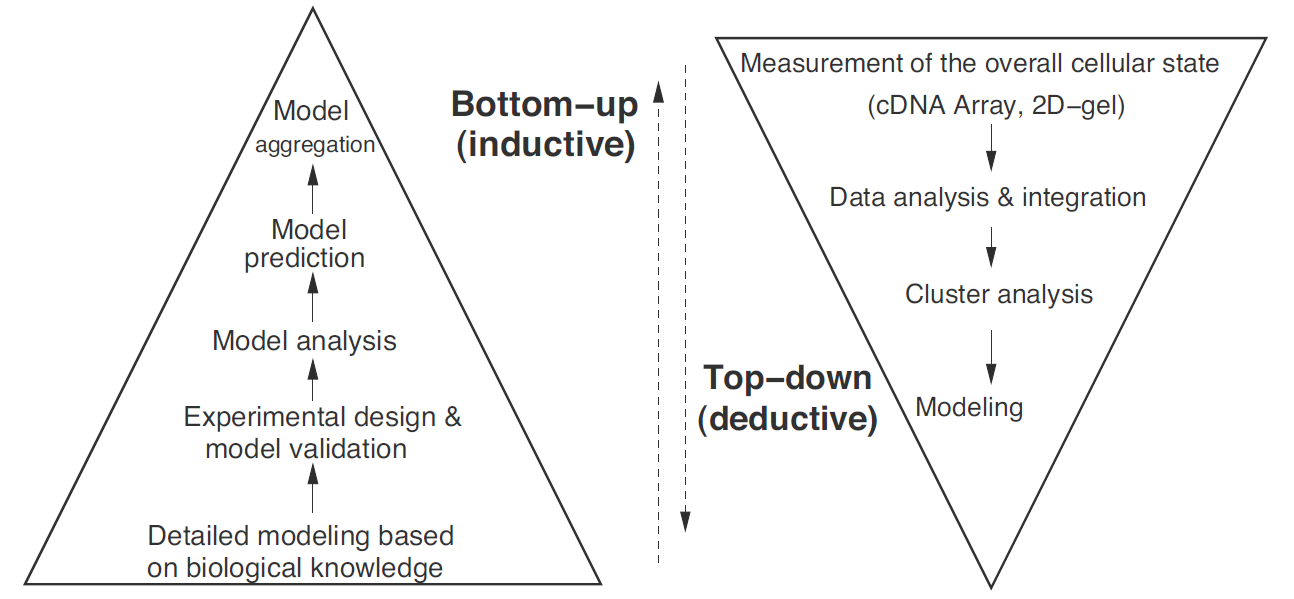
\includegraphics[width=0.8\columnwidth]{systemsbiology.png}
\end{center}
\caption[Systems biology approaches]{Systems biology approaches. Left: Bottom-up approach. Right: Top-down approach. Figure is taken from \cite{kremling2013systems}.}
\vskip\baselineskip % Leave a vertical skip below the figure
\label{fig:systemsbiology}
\end{figure}

\subsection{Metabolic Networks}
In the context of systems biology, metabolic network reconstructions have become a common interest for the researchers over the past 20 years \cite{thiele2010protocol}. Organism-specific metabolic network analyses allow scientists to design experiments and even obtain beforehand predictions. These networks are the main sources of the mathematical models which can simulate metabolic fluxes reflecting the experimantal reality \cite{orth2010flux}.

Before the improvement of genome sequencing or annotation technologies, initial core metabolic networks were based on the accessible information of biochemical pathways \cite{vallino1994carbon} \cite{varma1993biochemical}. In the last decade, larger genome-scale metabolic models (GSMMs) have been able to be developed rapidly with the help of databases for annotated genomes, providing information on substrates and products of each enzyme and each bioreaction \cite{feist2009reconstruction}. Growing biochemical databases provide automatization processes for the metabolic network reconstructions. As a result, genome-scale metabolic networks are available today for almost all organisms with an annotated genome available in the literature \cite{pitkanen2014comparative, kerkhoven2014applications}. From the first genome-scale metabolic model of \emph{Escherichia coli} to other organisms, the steps are required for GSMM development remained the same regardless of the biological diversity.

A generally applicable protocol is defined by the Palsson group \cite{thiele2010protocol, feist2009reconstruction} for the reconstruction of biochemical networks described in the Figure \ref{fig:modelreconstruction} \cite{chen2012metabolic}. Briefly, genomic data for the biochemical reactions of an organism are identified from the databases, such as NCBI, DDBJ and EMBL-EBI. Extraction and processing of the gene-protein-reaction relationship (GPR) of the genomic data results a draft reconstruction. GPR associations in the draft model should be reviewed by the researchers and manually curated if the identifying process is achieved with the help of automated computational algorithms \cite{pitkanen2014comparative}. Since the genomic data is the least representative of the biological phenotypes, available transcriptomic, proteomic, metabolomic and/or subcellular localization data are also used to further curate the model. Once the final metabolic network is reconstructed with bibliographic information, it is translated into a mathematical model.

\begin{figure}[ht]
\begin{center}
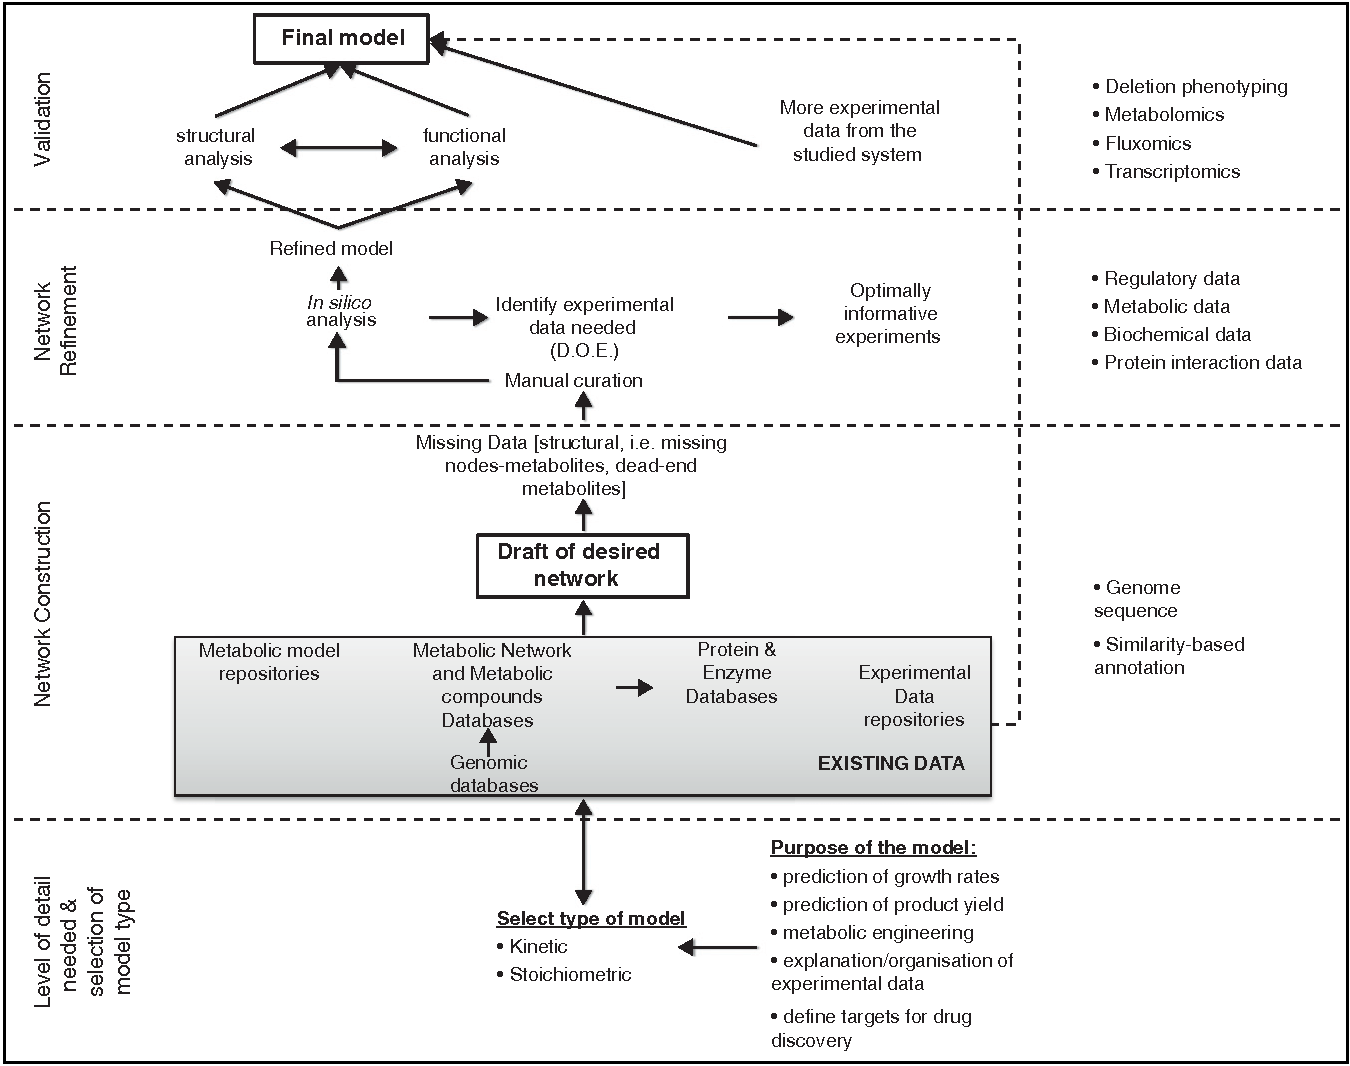
\includegraphics[width=1\columnwidth]{modelreconstruction.png}
\end{center}
\caption[Overview of metabolic network reconstruction protocol]{Overview of metabolic network reconstruction protocol. Figure is taken from \cite{chen2012metabolic}.}
\vskip\baselineskip % Leave a vertical skip below the figure
\label{fig:modelreconstruction}
\end{figure}

Once a metabolic network is reconstructed, a rational link between a genome sequence, the proteins encoded in the genome, and the reactions catalyzed by the proteins allowing to investigate the relationships between genotype and phenotype is achieved \cite{durot2008genome}. As the final step, GSMM needs to be validated by the new experimental data sets. GSMM validation process for various experimental conditions require detailed cultivation data from experiments. For example, information on the biomass composition of the specific organism leads more accurate biomass equation in the model, that is one of the key factors in the GSMM optimization and validation \cite{dikicioglu2015biomass}. Even tough multiple steps in the GSMM reconstruction can be achieved with the automated softwares available, it is usually necessary to curate the obtained model manually.

Approaches for analyzing metabolic networks are mainly categorized as dynamic or structural approaches. Even though the former is promising more realistic approach, its implementation in the literature is obstructed due to the unavailability of kinetic parameters for the majority of enzymes within a metabolic network \cite{machado2014systematic, ramkrishna2012dynamic} Because of the lack of kinetic parameters, structural metabolic modeling has been widely used for analyzing cellular metabolism at a steady-state assumption as a kind of snapshots taken at specific times.

GSMMs are one of the most useful tools in systems biology, especially in metabolic engineering studies \cite{kim2012recent}. In 1998, with the publication of \emph{Metabolic Engineering: Principles and Methodologies}, the term metabolic engineering is defined as the optimization of natural processes within cells to increase the production of certain substances \cite{stephanopoulos1999metabolic}. Hence, studies of metabolic engineering can be considered as genetic engineering in strain development. However, while metabolic engineering manipulates strains by altering flux distributions in the pathways; genetic engineering modificates specific genes, proteins and/or enzymes of interest \cite{stephanopoulos2012synthetic}. Although GSMMs are mainly used in metabolic engineering strategies, other applications both for descriptive and predictive purposes can be found in the literature \cite{osterlund2012fifteen}.

The ultimate goal of the GSMM reconstruction is to predict flux distribution profiles as close \emph{in silico} as they are \emph{in vivo}. Hence, GSMMs are in continuous research to improve predictability of organism-specific models.

\begin{figure}[ht]
\begin{center}
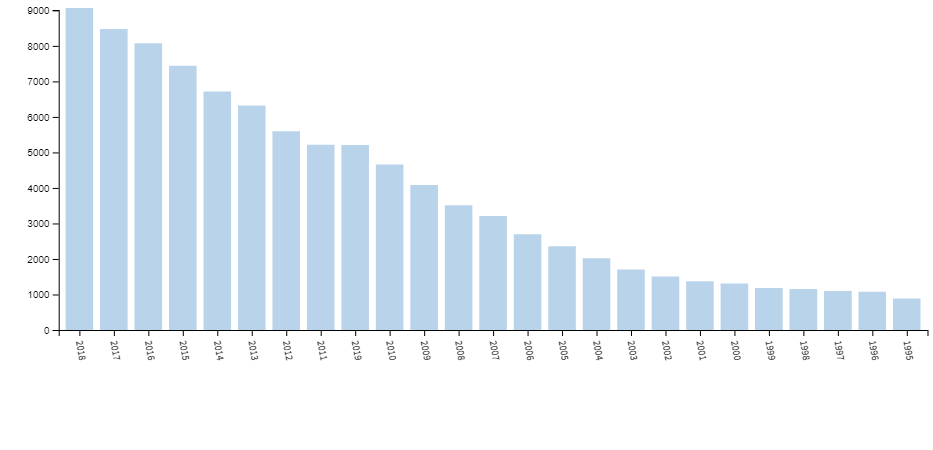
\includegraphics[width=1\columnwidth]{wos_metabolicmodel_search.jpg}
\end{center}
\caption[Web of Science artice counts on "metabolic model"]{Web of Science artice counts on "metabolic model"}
\label{fig:wos_metabolicmodel}
\end{figure}

\subsection{Mathematical Representation of Metabolic Networks}
\hl{In this section, there will be a review on} "Mathematical Framework Behind the Reconstruction and Analysis of Genome Scale Metabolic Models" \cite{pinzon2018mathematical}.

 This section will be detailed as much as possible since biology majors must understand the basics before reading the methods sections. How the biochemical equations are converted into differential equations? Steady state assumption, mass balances? Stoichiometric matrix formulation and its rank, linearly independent vectors, singular values? etc. Subjects will be similar to course ChE529.


\subsection{Constraint-Based Modeling}

\hl{In this section, there will be a review on} "Bringing genomes to life: the use of genome-scale in silico models" \cite{thiele2007bringing}.
Topics can be identification of constraints (physicochemical constraints, spatial constraints, environmental constraints, regulatory constraints), list of constraint-based modeling methods (optimal solutions, alternate optima, OptKnock, sampling as an unbiased modeling), linear programming, quadratic programming ...


\section{\emph{Saccharomyces cerevisiae}}

The species "yeast" includes a range of eukaryotic single-celled microorganisms, although it is commonly used to describe \emph{Saccharomyces cerevisiae}. Also known as the baker's yeast, \emph{S. cerevisiae} is one of the extensively used microorganisms for alcoholic fermentation of beverages, bio-ethanol production, and processing various foods since ancient times \cite{gelinas2009inventions}. It was the first eukaryotic organism whose genome was fully sequenced and annotated \cite{goffeau1997multidrug}, and besides its benefits in the industry, it is used as a model system for other eukaryotic cells including humans \cite{dujon1996yeast, botstein1997yeast}.

\subsection{Central Carbon Metabolism of \emph{S. cerevisiae}}
From the end of the eighteenth century, mainly after the fermentation is defined as "respiration without oxygen", the metabolism of \emph{S. cerevisiae} has been studied extensively \cite{barnett1998history, barnett2000history}. Its capability to produce ethanol is one of the most characterized microbial processes due to industrial utilization.

The set of anabolic and catabolic reactions in the cell are reffered as the metabolism. A shematic representation of the central carbon metabolism in \emph{S. cerevisiae} can be found in Figure \ref{fig:central_carbon_mech_of_s_cerevisiae_kegg}. Glycolysis, pentose-phosphate pathway (PPP), tricarboxylic acid cycle (TCA) or Krebs cycle, the glyoxylate cycle and the electron transport chain are the main pathways in central carbon metabolism.

 \begin{figure}[ht]
 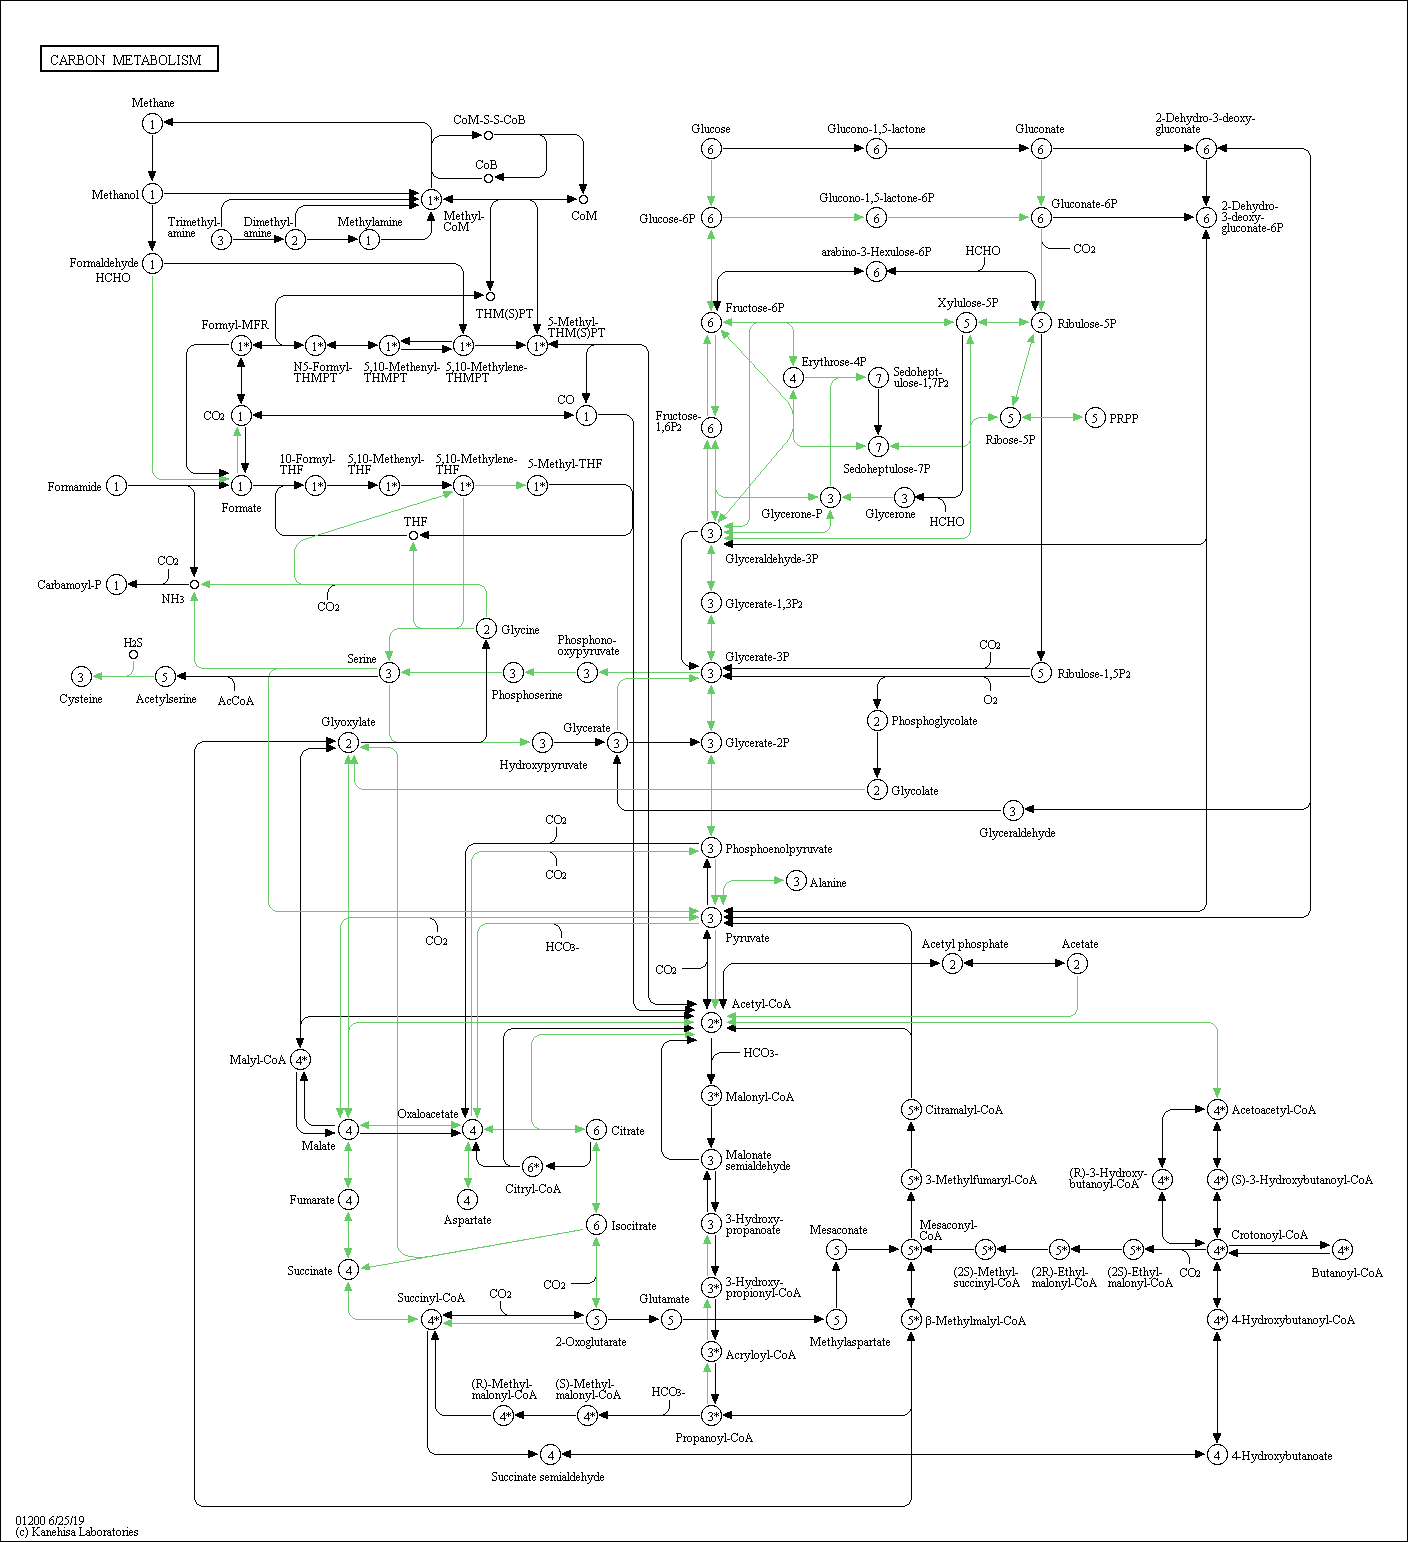
\includegraphics[width=1\columnwidth]{central_carbon_mech_of_s_cerevisiae_kegg.png}
 \caption[Central carbon mechanism of \emph{S. cerevisiae}]{Central carbon mechanism of \emph{S. cerevisiae} obtained from  KEGG \cite{kanehisa2000kegg}.}
 \vskip\baselineskip % Leave a vertical skip below the figure
 \label{fig:central_carbon_mech_of_s_cerevisiae_kegg}
 \end{figure}

\hl{In this section, there will be subsections on} all biological pathways individually (explaining each in detail -probably referencing Lehninger biochemistry-) especially NAD regulation, fermantation (crabtree effect, industrial applications, bio-ethanol production) etc... Maybe also regulation strategies in cells (feedback/feedforward loops with figures)

\subsection{Adaptive Evolution Studies on \emph{S. cerevisiae} (Palsson 2015)}

\subsection{Metabolic Models of \emph{S. cerevisiae}}
After the first \emph{S. cerevisiae} genome sequence is published, the first cDNA spotted microarray exploring metabolic gene regulation in 1997 \cite{derisi1997exploring}, and the first commercial platform for oligonucleotide microarray data (Affymetrix) to investigate cellular regulations were reported in 1998 \cite{cho1998parallel}. Existing genome data is integrated with the extensive annotation based on microarray data and biochemical knowledge from literature, leading of the publication of the first GSMM of \emph{S. cerevisiae} in 2013 \cite{forster2003genome}.   \hl{More in this section, there will be review on:} Genome-scale modeling of yeast: chronology, applications and critical perspectives \cite{lopes2017genome}

\subsection{Applications of \emph{S. cerevisiae} GSMMs}
 \hl{Literature review on the applications will be added.}

%	\input{chapters/chapters_overall}
	\chapter{MATERIALS AND METHODS - Yeast8}

\section{Consensus \emph{S. cerevisiae} Metabolic Model}
Variety of \emph{S. cerevisiae} genome-scale metabolic models have been used since 2003, and each reconstructed model introduced more manual curations, increasing gene numbers from annotations and better predictions regarding the previous ones \cite{lopes2017genome}. A consensus genome-scale metabolic model of \emph{S. cerevisiae}, Yeast8, is presented in an open-source, version-controlled maintainable way in 2019, claiming that the model can be represented and investigated in a systematic way using Git (https://git-scm.com/) and GitHub (https://github.com/) as a hosting service for the model repository \cite{lu2019consensus}. Systematic way of Yeast8 enables to study simultaneously in collaborative studies, provides record keeping of model changes, version updates, where each version of can be released periodically and accessible all the time (Figure \ref{fig:yeast8_github}).
\begin{figure}[ht]
\begin{center}
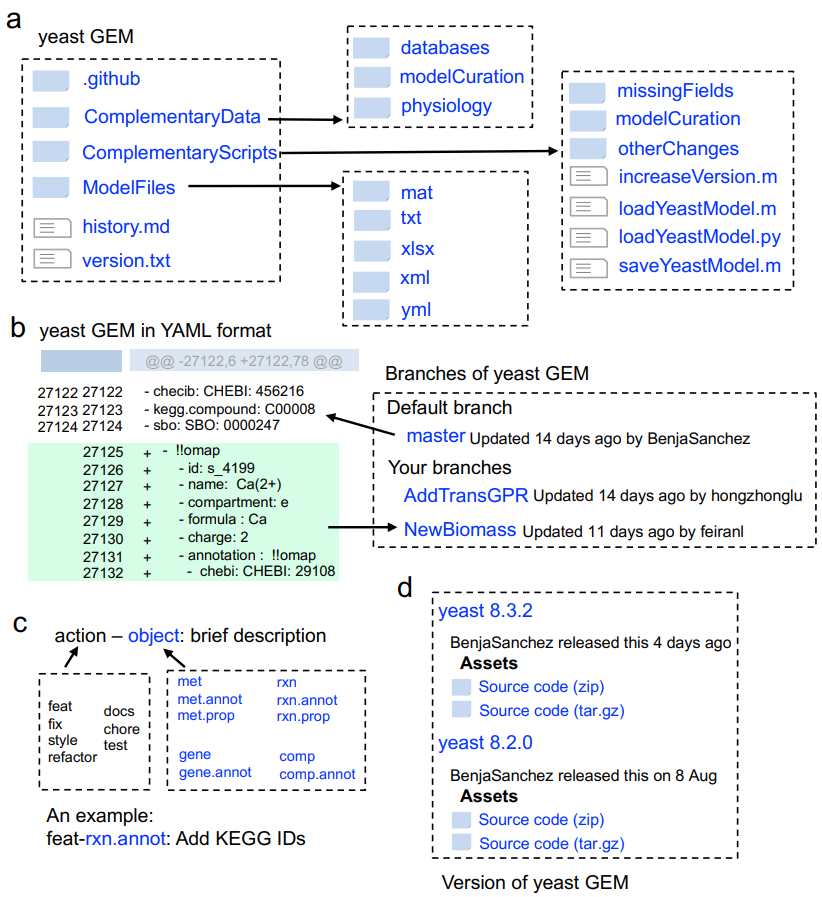
\includegraphics[width=0.9\columnwidth]{yeast8_github.png}
\end{center}
\caption[Repository of yeast GEM on GitHub]{Repository of yeast GEM on GitHub. Figure is taken from \cite{lu2019consensus}. ~ will be redrawned in thesis}
\label{fig:yeast8_github}
\end{figure}

Yeast8 model can be considered as an updated version of Yeast7 \cite{aung2013revising} with additional corrections based on the annotations available in KEGG and ChEBI, and several gene inclusions from the model iSce926 \cite{chowdhury2015using}. Final version of Yeast8, version 8.3.4 released on July 28, has 3991 reactions, 2691 metabolites, 1149 genes, 14 intracellular compartments.

All simulations in this chapter are done using Yeast8 v8.3.4 model which is hosted in Github (https://github.com/SysBioChalmers/yeast-GEM).

\section{Chemostat Simulation: GAM Fitting}
In order to make sure the \emph{in-silico} obtained growth rate predictions are in agreement with the physiological kinetic parameters obtained from real experiments, fine adjustment on the energy reactions is a requirement. Since the growth-associated maintenance (GAM) and non-growth associated maintenance (NGAM) energy reactions play a determinant role in simulations, fluxes through these reactions must be constrained to a fixed value. Flux of NGAM is constrained to 0.7 mmol gDWh\textsuperscript{-1} for aerobic, and 0 mmol gDWh\textsuperscript{-1} for anaerobic simulations as calculated in the previous studies \cite{nilsson2016metabolic}. For the estimatation of GAM, since it depends on the biomass composition, findings of a chemostat experiment \cite{van1998effect} is used as a guide to fit predictions to. Model is simulated iteratively with a range of values for GAM, and the best fit is found at the level of 55.25 mmol gDWh\textsuperscript{-1} (Figure \ref{fig:Gam_fitting}), GAM flux is constrained accordingly.

\begin{figure}
\begin{center}
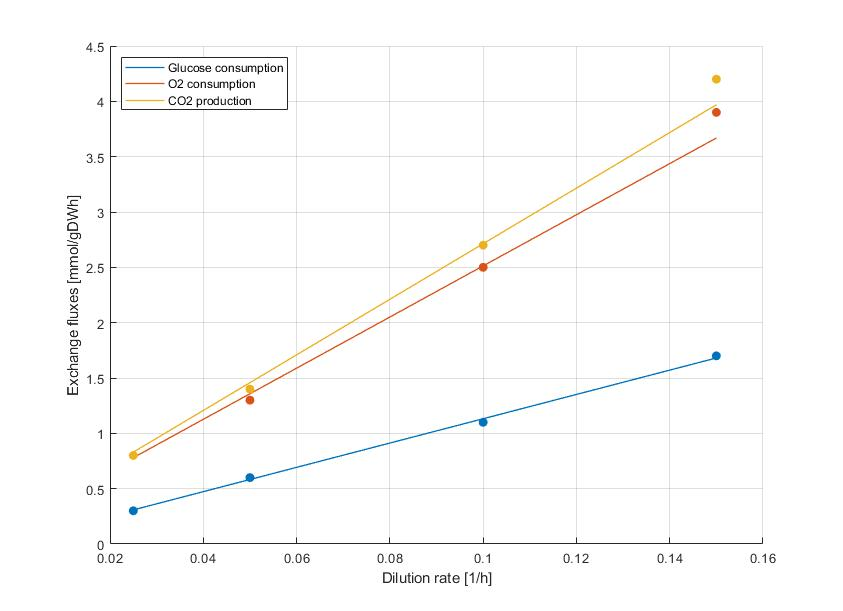
\includegraphics[width=0.8\columnwidth]{Gam_fitting.jpg}
\end{center}
\caption[Chemostat simulation to re-fit growth associated maintenance]{Chemostat simulation to re-fit growth associated maintenance.}
\label{fig:Gam_fitting}
\end{figure}


\section{Flux Balance Analysis}
Mathematical background of FBA...\hl{Review on "What is FBA?"}

In order to simulate batch conditions where minimal yeast medium is used, all the exchange reactions in the model are blocked first (lower bounds are set to 0). Then, only the exchange reactions of ions that are available to the cells in the experimental design (ammonium, phosphate, sulphate, iron(2+), H+, water, chloride, Mn\textsuperscript{2+}, Zn\textsuperscript{2+}, Mg\textsuperscript{2+}, sodium, Cu2\textsuperscript{2+}, Ca\textsuperscript{2+}, potassium) are set free (lower bounds are set to -1000). While oxygen and glucose uptake rates decreasing from 20 mmol gDWh\textsuperscript{-1} and increasing to 20 mmol gDWh\textsuperscript{-1}, respectively, fluxes on ethanol, acetate, glycerol, formate, succinate secretion reactions and growth rate is collected (Figure \ref{fig:fba}).
\hl{I need to show experimental results -preferably from the same article where I got expression data- on the figure to compare with my FBA results}


\begin{figure}
\begin{center}
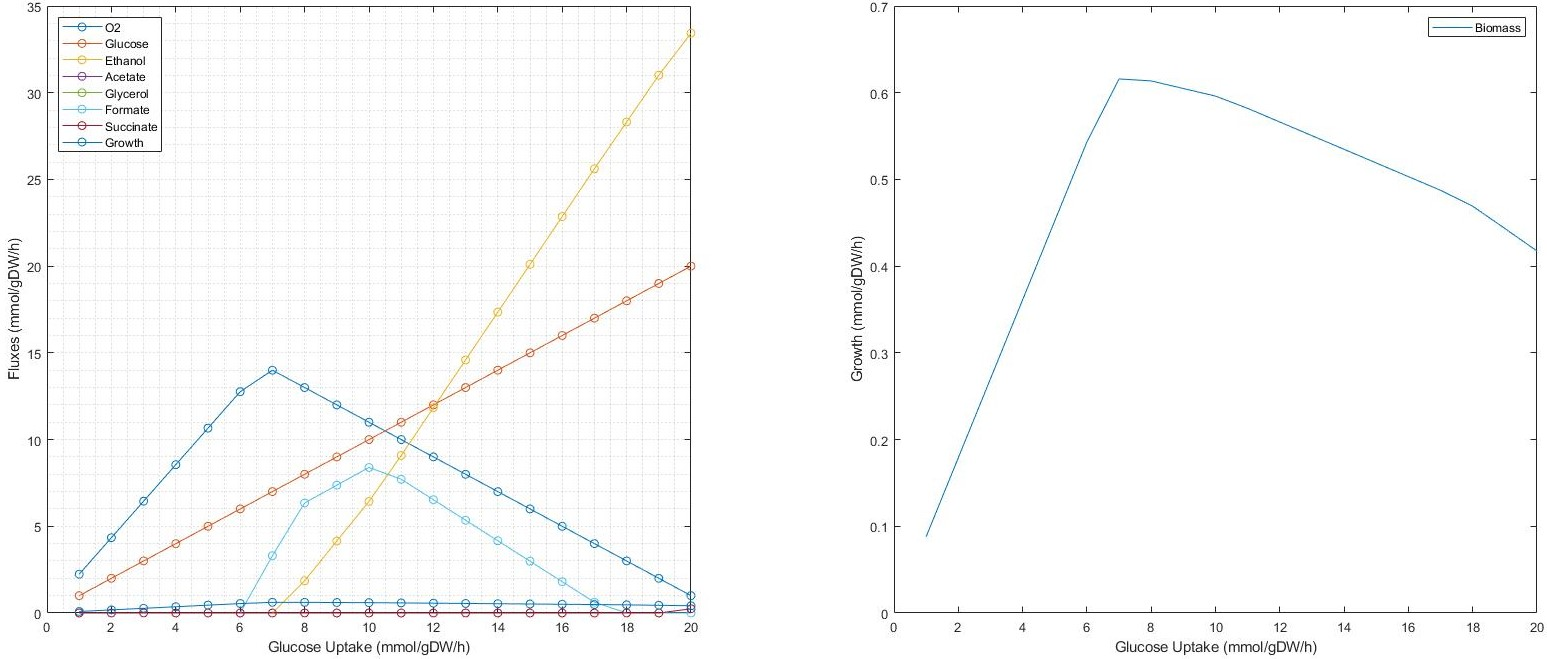
\includegraphics[width=1\columnwidth]{fba.jpg}
\end{center}
\caption[Flux balance simulation results]{Flux balance simulation results where oxygen uptake rate decreased and glucose uptake rate is increased simultaneously. Flux rates of several metabolites on the left, predicted growth rate on the right.}
\label{fig:fba}
\end{figure}


\section{Flux Variability Analysis}
Flux variability analysis (FVA) determines the minimum and maximum available fluxes for each reaction while obeying the provided constraints (for example fixed glucose uptake or growth rate). FVA is mainly used to evaluate the robustness of the model \cite{thiele2010functional}, to find alternative optimum states \cite{mahadevan2003effects}, to check flux distributions when growth is not at optimum level \cite{reed2004genome}, and in many other applications \cite{gudmundsson2010computationally}.


(Figure \ref{fig:fva})

\begin{figure}
\begin{center}
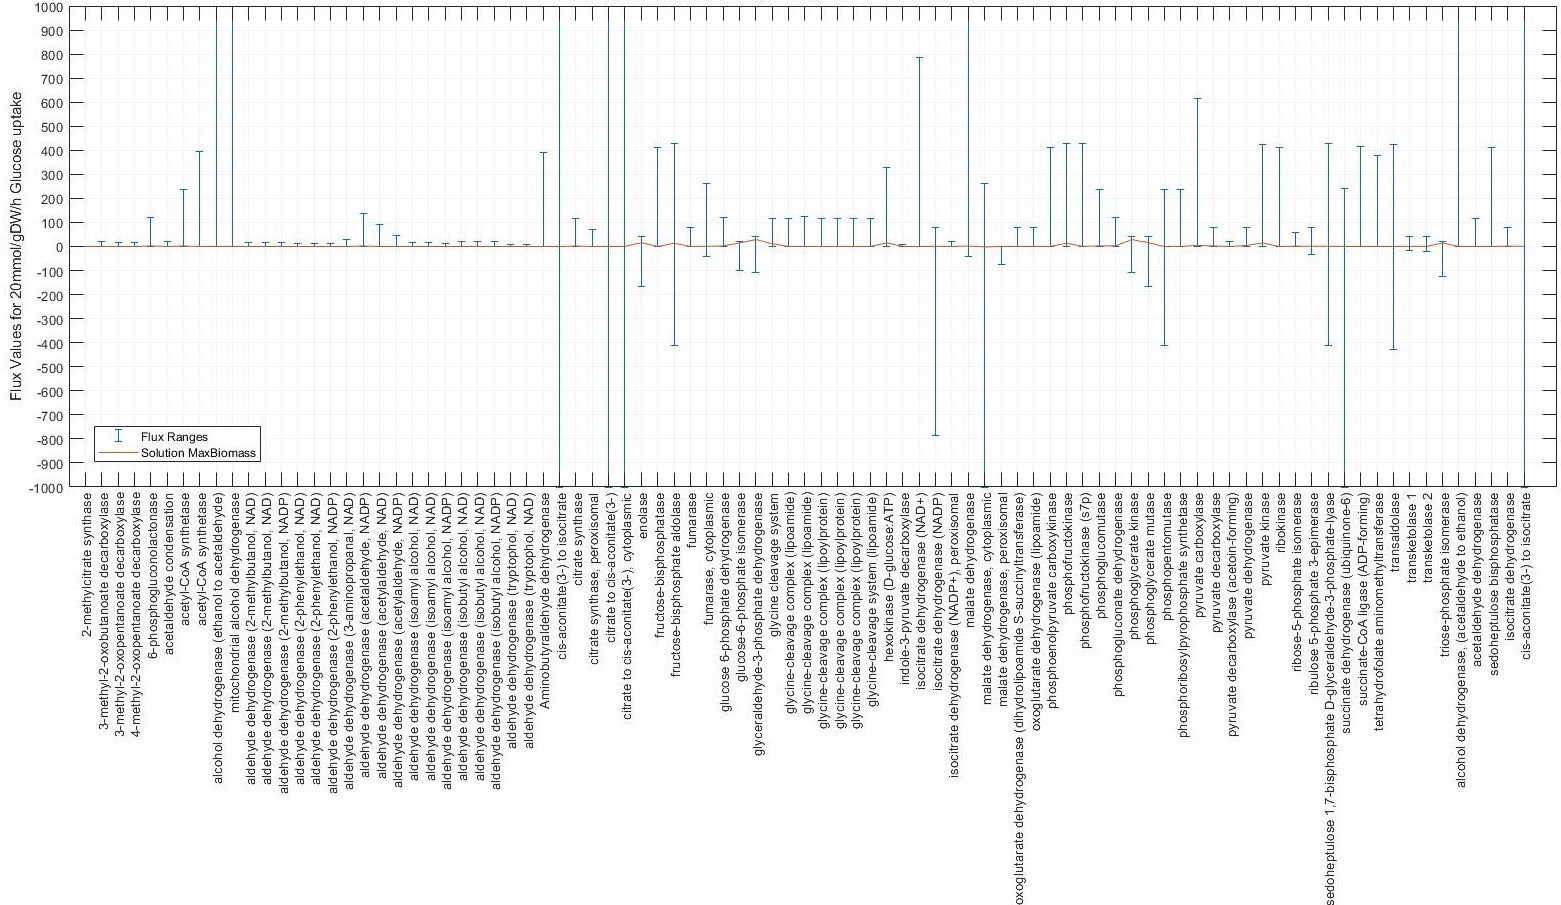
\includegraphics[width=1\columnwidth]{fva.jpg}
\end{center}
\caption[Minimum and maximum fluxes of Glycolysis, PPP and TCA reactions]{Minimum and maximum fluxes of Glycolysis, PPP and TCA reactions.}
\label{fig:fva}
\end{figure}

\section{Phenotype Phase Plane Construction}
\section{ACHRB Sampling}
\section{Expression Data Analysis}
\section{Integration of Expression Data Into Model}

	\chapter{MATERIALS AND METHODS - Petek}

\section{Experimental Data Preparation}
\subsection{Data Acquisition}
Extracellular metabolomics data is obtained from Cakar's Lab \cite{arslan2018physiological}.Briefly, they perform ethyl methane sulfonate (EMS) mutagenesis  on the prototrophic \emph{Saccharomyces cerevisiae} strain CEN.PK 113-7D (MATa, MAL2-8c, SUC2) to increase the genetic diversity as an evolutionary engineering selection strategy. Cells were inoculated in 2\% Yeast Minimal Media (YMM), and the extracellular concentrations of glucose, ethanol, glycerol and acetate were measured at different time points. OD\textsubscript{600} values were determined by a spectrophotometer. Additionally, cell dry weight analysis was conducted to determine biomass production. Acquired extracellular metabolite concentrations, OD\textsubscript{600} values and dry weights of the reference strain (without mutagenesis) were used in this study are collected in Table \ref{table:experimental_data} and Table \ref{table:experimental_OD600s_and_growths}.

\begin{table}[H]
\caption[Measured OD\textsubscript{600} and cell dry weight values of reference strain \cite{surmeli2019evolutionary}]{Measured OD\textsubscript{600} and cell dry weight values of reference strain \cite{surmeli2019evolutionary}.}
\begin{center}
  \begin{tabular}{|c|c|c|c|}
 \hline
  \textbf{Time (h)} & \textbf{OD600} & \textbf{ln(OD600)} & \textbf{Cell DW (g/L)} \\
  \hline
  0                 & 0.21           & -1.560647748       & -                      \\
  3                 & 0.53           & -0.634878272       & -                      \\
  6                 & 1.76           & 0.565313809        & 0.9                    \\
  7.5               & 2.66           & 0.978326123        & -                      \\
  9                 & 4.46           & 1.495148766        & 1.9                    \\
  12                & 5.31           & 1.669591835        & -                      \\
  15                & 5.88           & 1.771556762        & -                      \\
  18                & 5.83           & 1.763017           & 2.32                   \\
  21                & 6.07           & 1.803358605        & -                      \\
  24                & 5.87           & 1.769854634        & -                      \\
  30                & 6.14           & 1.814824742        & 2.26                   \\
  40                & 6.44           & 1.86252854         & -                      \\
  46                & 6.36           & 1.850028377        & -                      \\
  50                & 6.3            & 1.840549633        & -                      \\
  54                & 6.55           & 1.87946505         & -                      \\
  63                & 6.54           & 1.877937165        & -                      \\
  67                & 6.88           & 1.928618652        & -                      \\
  72                & 6.97           & 1.941615225        & 2.66                  \\
   \hline
  \end{tabular}
\label{table:experimental_OD600s_and_growths}
\end{center}
\end{table}

\begin{table}[H]
\caption[Measurements of extracellular concentrations \cite{surmeli2019evolutionary}]{Measurements of extracellular concentrations \cite{surmeli2019evolutionary}.}
\begin{center}
\begin{tabular}{|c|c|c|c|c|}
   \hline
  \textbf{Time(h)} & \textbf{Glucose(g/L)} & \textbf{Ethanol(g/L)} & \textbf{Glycerol(g/L)} & \textbf{Acetate(g/L)} \\
    \hline
  0                 & 19.99            & 0                & 0                 & 1.08             \\
  3                 & 17.98            & 0.58             & 0.02              & 1.24             \\
  6                 & 15.85            & 1.2              & 0.06              & 1.16             \\
  9                 & 12.21            & 3.39             & 0.18              & 1.37             \\
  12                & 9.18             & 7.97             & 0.61              & 2.45             \\
  15                & 0.4              & 8.17             & 0.69              & 2.46             \\
  27                & 0                & 8.28             & 0.76              & 2.6              \\
  46                & 0                & 8                & 0.77              & 2.45             \\
  50                & 0                & 6.62             & 0.64              & 2.02             \\
  54                & 0                & 5.74             & 0.55              & 1.73             \\
  58                & 0                & 5.46             & 0.54              & 1.74             \\
  72                & 0                & 3.72             & 0.49              & 1.33            \\
   \hline
\end{tabular}
\label{table:experimental_data}
\end{center}
\end{table}


\subsection{Determination of Rates}
As the slope in the curve of lnOD\textsubscript{600} as a function of time gives the growth rates of cells, natural logarithm of OD\textsubscript{600} values were calculated to obtain specific growth rates by using the equation \ref{eq:growthrates}.
  \begin{equation}
      \ \mu = \frac{\Delta \ln{OD_{600}}}{\Delta t}
      \label{eq:growthrates}
  \end{equation}

In order to determine uptake and secretion rates of the metabolites, the steady-state assumption is applied in three hours intervals as the shortest measured time-points. Missing data on cell dry weights are estimated from the OD\textsubscript{600} values, and these cell dry weight data is used to calculate fluxes (in the unit of mmol/gDWh). Measurement of the cell dry weight at the 3rd hour was crucial for the steady-state assumption, however data was not available from the experiments. Curve trend of the OD\textsubscript{600} plot is used as a guide to estimate cell dry weight (Figure \ref{fig:GrowthGraphs}) \hl{Need a method here: Estimation approach, maybe regression or curve fitting?}. Calculated flux values can be found in the Table \ref{table:calculated_fluxes}.
\begin{figure}[H]
  \begin{center}
  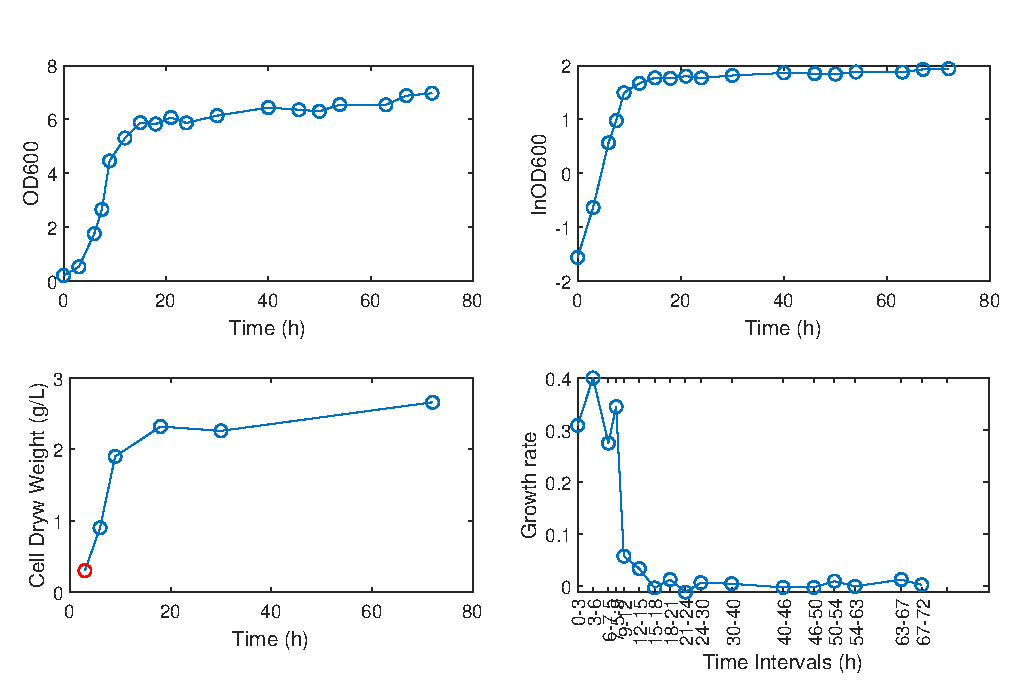
\includegraphics[width=1\columnwidth]{GrowthGraphsSmall.eps}
  \end{center}
  \caption[OD\textsubscript{600}, lnOD\textsubscript{600}, cell dry weights and growth rates]{OD\textsubscript{600}, lnOD\textsubscript{600}, cell dry weights and growth rates graphs. Estimated missing cell dry weight data is shown in red color.}
\label{fig:GrowthGraphs}
\end{figure}

\begin{table}[thbp]
\vskip\baselineskip
\caption[Calculated flux values]{Calculated flux values.}
\begin{center}
  \begin{tabular}{cccccc}
  \multicolumn{1}{l}{\textbf{Time}} & \multicolumn{4}{c}{\textbf{Metabolite fluxes in mmol/gDWh}}                & \textbf{Growth h-1} \\
  \textbf{}                         & \textbf{Glucose} & \textbf{Ethanol} & \textbf{Glycerol} & \textbf{Acetate} & \textbf{Biomass}    \\
  0-3                               & -12.3963884      & 13.98837518      & 0.24131           & 2.960496         & 0.30859             \\
  3-6                               & -4.378823762     & 4.984363569      & 0.160873          & -0.49342         & 0.400064
  \end{tabular}
\label{table:calculated_fluxes}
\end{center}
\end{table}


\section{Model Selection}
iAN50 \cite{nilsson2016metabolic}, a stoichiometric model of intermediary metabolism including glycolysis, the pentose phosphate pathway (PPP), anaerobic excretion, citric acid cycle (TCA cycle), oxidative phosphorylation, and uptake pathways for galactose, ethanol and acetate is used to simulate batch conditions. The model was implemented based on the first GSMM of yeast, iFF708 \cite{forster2003genome} with the addition of the yeast intermediary metabolism from the RAVEN toolbox \cite{agren2013raven}, and finally curated using the KEGG database \cite{kanehisa2000kegg}.

Biomass equation (Eq. \ref{eq:model_biomass}) in the model was left as a function of sub-reactions, for example protein, lipid, DNA synthesis reactions, so that the coefficients of biomass constituents could be optimized for each FBA simulation.
\begin{multline}
  0.5185\ \textrm{Glycogen} + 0.0234\ \textrm{Trehalose} + 0.8079\ \textrm{Mannan} + 1.1348\ \textrm{Glucan} \\
  + 0.1966\ \textrm{DNA} + 0.012\ \textrm{DNA} +  4.14\ \textrm{Protein} + 0.0269\ \textrm{Lipid} + 35.3630 \ \textrm{Maintainance} \\
  = \textrm{BIOMASS}
   \label{eq:model_biomass}
\end{multline}

Enzymatic reactions that are found in the model is collected in Table \ref{table:rxns_smallYeast}. In contrast to other GSMM's, each reaction was irreversible in the iAN50. This was achieved by splitting each reversible reaction into two seperate reactions in both directions.

Another reason to select iAN50 is that the total masses of enzymes catalyzing reactions in the GSMM were already estimated, and fluxes through these reactions were constrained to the biologic level, using an approach similar to intracellular crowding method using kinetic parameters \cite{beg2007intracellular, adadi2012prediction}. To clarify the method briefly, a flux value for each reaction was obtained by applying a standart flux balance analysis, and this value was divided by the maximum \emph{in vitro} activity collected from the enzyme database BRENDA \cite{schomburg2012brenda}, and a saturation factor of 0.5 (half) for simplification. Therefore, the mass of the enzymes required for that particular reaction was estimated and the constrains are applied to the corresponding enzymatic reactions.

\begin{table}[H]
\vskip\baselineskip
  \caption[Reaction list in the iAN50 model]{Reaction list in the iAN50 model.}
  \begin{center}
\resizebox{\textwidth}{!}{
\begin{tabular}{p{11cm}p{17cm}p{8cm}lp{5cm}}
\hline
\textbf{NAME}                                                                             & \textbf{EQUATION}                                                                                                                               & \textbf{GENE ASSOCIATION}                                                                                                                                        & \textbf{EC-NUMBER} & \textbf{SUBSYSTEM}                                                          \\ \hline
Hexokinase                                                                                & GLC{[}c{]} + ATP{[}c{]} =\textgreater ADP{[}c{]} + G6P{[}c{]}                                                                                   & YFR053C; YGL253W; YCL040W                                                                                                                                        & 2.7.1.1 OR 2.7.1.2 & Glycolysis                                                                  \\
Glucose-6-phosphate isomerase                                                             & G6P{[}c{]} \textless{}=\textgreater F6P{[}c{]}                                                                                                  & YBR196C                                                                                                                                                          & 5.3.1.9            & Glycolysis                                                                  \\
Phosphofructokinase                                                                       & ATP{[}c{]} + F6P{[}c{]} =\textgreater ADP{[}c{]} + F16P{[}c{]}                                                                                  & YGR240C; YMR205C                                                                                                                                                 & 2.7.1.11           & Glycolysis                                                                  \\
Fructose-1,6-bisphosphatase                                                               & F16P{[}c{]} =\textgreater F6P{[}c{]} + PI{[}c{]}                                                                                                & YLR377C                                                                                                                                                          & 3.1.3.11           & Glycolysis                                                                  \\
Fructose-bisphosphate aldolase                                                            & F16P{[}c{]} \textless{}=\textgreater GA3P{[}c{]} + DHAP{[}c{]}                                                                                  & YKL060C                                                                                                                                                          & 4.1.2.13           & Glycolysis                                                                  \\
Triosephosphate isomerase                                                                 & DHAP{[}c{]} \textless{}=\textgreater GA3P{[}c{]}                                                                                                & YDR050C                                                                                                                                                          & 5.3.1.1            & Glycolysis                                                                  \\
Triosephosphate dehydrogenase                                                             & GA3P{[}c{]} + NAD{[}c{]} + PI{[}c{]} \textless{}=\textgreater P13G{[}c{]} + NADH{[}c{]}                                                         & YJL052W; YJR009C; YGR192C                                                                                                                                        & 1.2.1.12           & Glycolysis                                                                  \\
Phosphoglycerate kinase                                                                   & P13G{[}c{]} + ADP{[}c{]} \textless{}=\textgreater P3G{[}c{]} + ATP{[}c{]}                                                                       & YCR012W                                                                                                                                                          & 2.7.2.3            & Glycolysis                                                                  \\
Phosphoglycerate mutase                                                                   & P3G{[}c{]} \textless{}=\textgreater P2G{[}c{]}                                                                                                  & YKL152C; YDL021W; YOL056W                                                                                                                                        & 5.4.2.11           & Glycolysis                                                                  \\
Enolase                                                                                   & P2G{[}c{]} \textless{}=\textgreater PEP{[}c{]}                                                                                                  & YGR254W; YHR174W; YOR393W; YPL281C; YMR323W                                                                                                                      & 4.2.1.11           & Glycolysis                                                                  \\
Pyruvate kinase                                                                           & ADP{[}c{]} + PEP{[}c{]} =\textgreater ATP{[}c{]} + PYR{[}c{]}                                                                                   & YOR347C; YAL038W                                                                                                                                                 & 2.7.1.40           & Glycolysis                                                                  \\
Glucose-6-phosphate 1-dehydrogenase                                                       & G6P{[}c{]} + NADP{[}c{]} =\textgreater G15L{[}c{]} + NADPH{[}c{]}                                                                               & YNL241C                                                                                                                                                          & 1.1.1.49           & Pentose Phosphate                                                           \\
6-phosphogluconolactonase                                                                 & G15L{[}c{]} =\textgreater P6G{[}c{]}                                                                                                            & YNR034W; YCR073W-A; YHR163W; YGR248W                                                                                                                             & 3.1.1.31           & Pentose Phosphate                                                           \\
6-phosphogluconate dehydrogenase, decarboxylating                                         & P6G{[}c{]} + NADP{[}c{]} =\textgreater CO2{[}c{]} + RU5P{[}c{]} + NADPH{[}c{]}                                                                  & YGR256W; YHR183W                                                                                                                                                 & 1.1.1.44           & Pentose Phosphate                                                           \\
ribose 5-phosphate isomerase                                                              & RU5P{[}c{]} \textless{}=\textgreater R5P{[}c{]}                                                                                                 & YOR095C                                                                                                                                                          & 5.3.1.6            & Pentose Phosphate                                                           \\
Ribulose-phosphate 3-epimerase                                                            & RU5P{[}c{]} \textless{}=\textgreater X5P{[}c{]}                                                                                                 & YJL121C                                                                                                                                                          & 5.1.3.1            & Pentose Phosphate                                                           \\
Transketolase                                                                             & R5P{[}c{]} + X5P{[}c{]} \textless{}=\textgreater GA3P{[}c{]} + S7P{[}c{]}                                                                       & YBR117C; YPR074C                                                                                                                                                 & 2.2.1.1            & Pentose Phosphate                                                           \\
Transaldolase                                                                             & GA3P{[}c{]} + S7P{[}c{]} \textless{}=\textgreater F6P{[}c{]} + E4P{[}c{]}                                                                       & YLR354C                                                                                                                                                          & 2.2.1.2            & Pentose Phosphate                                                           \\
Transketolase                                                                             & E4P{[}c{]} + X5P{[}c{]} \textless{}=\textgreater F6P{[}c{]} + GA3P{[}c{]}                                                                       & YBR117C; YPR074C                                                                                                                                                 & 2.2.1.1            & Pentose Phosphate                                                           \\
Pyruvate carboxylase 1                                                                    & ATP{[}c{]} + CO2{[}c{]} + PYR{[}c{]} =\textgreater ADP{[}c{]} + OAA{[}c{]} + PI{[}c{]}                                                          & YGL062W; YBR218C                                                                                                                                                 & 6.4.1.1            & TCA                                                                         \\
Citrate synthase, mitochondrial                                                           & ACCOA{[}m{]} + OAA{[}m{]} =\textgreater CI{[}m{]} + COA{[}m{]}                                                                                  & YNR001C; YPR001W                                                                                                                                                 & 2.3.3.1            & TCA                                                                         \\
Aconitate hydratase, mitochondrial                                                        & CI{[}m{]} \textless{}=\textgreater ICI{[}m{]}                                                                                                   & YLR304C                                                                                                                                                          & 4.2.1.3            & TCA                                                                         \\
Isocitrate dehydrogenase                                                                  & ICI{[}m{]} + NAD{[}m{]} =\textgreater AKG{[}m{]} + CO2{[}m{]} + NADH{[}m{]}                                                                     & YNL037C; YOR136W                                                                                                                                                 & 1.1.1.41           & TCA                                                                         \\
Isocitrate dehydrogenase {[}NADP{]}, mitochondrial                                        & ICI{[}m{]} + NADP{[}m{]} =\textgreater AKG{[}m{]} + CO2{[}m{]} + NADPH{[}m{]}                                                                   & YDL066W; YLR174W                                                                                                                                                 & 1.1.1.42           & TCA                                                                         \\
Alpha-ketoglutarate dehydrogenase                                                         & AKG{[}m{]} + NAD{[}m{]} + ADP{[}m{]} + PI{[}m{]} =\textgreater CO2{[}m{]} + NADH{[}m{]} + ATP{[}m{]} + SUC{[}m{]}                               & YDR148C; YIL125W                                                                                                                                                 & 1.2.4.2            & TCA                                                                         \\
Succinate dehydrogenase complex                                                           & FAD{[}m{]} + SUC{[}m{]} =\textgreater FADH2{[}m{]} + FUM{[}m{]}                                                                                 & YKL148C; YLL041C                                                                                                                                                 & 1.3.5.1            & TCA                                                                         \\
Fumarate reductase                                                                        & FADH2{[}m{]} + FUM{[}m{]} =\textgreater FAD{[}m{]} + SUC{[}m{]}                                                                                 & YJR051W; YEL047C                                                                                                                                                 & 1.3.1.6            & TCA                                                                         \\
Fumarate hydratase                                                                        & FUM{[}m{]} \textless{}=\textgreater MAL{[}m{]}                                                                                                  & YPL262W                                                                                                                                                          & 4.2.1.2            & TCA                                                                         \\
Malate dehydrogenase                                                                      & MAL{[}m{]} + NAD{[}m{]} \textless{}=\textgreater NADH{[}m{]} + OAA{[}m{]}                                                                       & YKL085W                                                                                                                                                          & 1.1.1.37           & TCA                                                                         \\
Galactokinase                                                                             & GAL{[}c{]} + ATP{[}c{]} =\textgreater GALP{[}c{]} + ADP{[}c{]}                                                                                  &                                                                                                                                                                  & 2.7.1.6            & Galactose metabolism                                                        \\
UDP-glucose 4-epimerase                                                                   & GALUDP{[}c{]} \textless{}=\textgreater GLUUDP{[}c{]}                                                                                            &                                                                                                                                                                  & 5.1.3.2            & Galactose metabolism                                                        \\
Galactose-1-phosphate uridylyltransferase                                                 & GLUUDP{[}c{]} + GALP{[}c{]} \textless{}=\textgreater G1P{[}c{]} + GALUDP{[}c{]}                                                                 &                                                                                                                                                                  & 2.7.7.12           & Galactose metabolism                                                        \\
Phosphoglucomutase-1                                                                      & G1P{[}c{]} \textless{}=\textgreater G6P{[}c{]}                                                                                                  &                                                                                                                                                                  & 5.4.2.2            & Galactose metabolism                                                        \\
glycerol-3-phosphate dehydrogenase                                                        & DHAP{[}c{]} + NADH{[}c{]} =\textgreater GP{[}c{]} + NAD{[}c{]}                                                                                  & YDL022W; YOL059W                                                                                                                                                 & 1.1.1.8            & Anaerobic excretion                                                         \\
sn-glycerol-3-phosphate phosphohydrolase                                                  & GP{[}c{]} =\textgreater GLY{[}c{]} + PI{[}c{]}                                                                                                  & YER062C; YIL053W                                                                                                                                                 & 3.1.3.21           & Anaerobic excretion                                                         \\
Pyruvate decarboxylase                                                                    & PYR{[}c{]} =\textgreater ACA{[}c{]} + CO2{[}c{]}                                                                                                & YGR087C; YLR134W; YLR044C                                                                                                                                        & 4.1.1.1            & Anaerobic excretion                                                         \\
Alcohol dehydrogenase                                                                     & ACA{[}c{]} + NADH{[}c{]} \textless{}=\textgreater ETH{[}c{]} + NAD{[}c{]}                                                                       & YGL256W; YMR303C; YOL086C                                                                                                                                        & 1.1.1.1            & Anaerobic excretion                                                         \\
Aldehyde dehydrogenase                                                                    & ACA{[}c{]} + NADP{[}c{]} =\textgreater AC{[}c{]} + NADPH{[}c{]}                                                                                 & YPL061W                                                                                                                                                          & 1.2.1.3            & Anaerobic excretion                                                         \\
Aldehyde dehydrogenase {[}NAD(P)+{]} 1                                                    & ACA{[}c{]} + NAD{[}c{]} =\textgreater NADH{[}c{]} + AC{[}c{]}                                                                                   & YMR170C; YMR169C; YOR374W; YOR374W; YER073W                                                                                                                      & 1.2.1.5            & Aromatic amino acid biosynthesis \\
Isocitrate lyase                                                                          & ICI{[}m{]} =\textgreater Glyoxylate{[}m{]} + SUC{[}m{]}                                                                                         & YER065C; YPR006C                                                                                                                                                 & 4.1.3.1            & Anaplerotic reactions                                                       \\
Malate synthase 1, glyoxysomal                                                            & ACCOA{[}m{]} + Glyoxylate{[}m{]} =\textgreater COA{[}m{]} + MAL{[}m{]}                                                                          & YIR031C; YNL117W                                                                                                                                                 & 2.3.3.9            & Anaplerotic reactions                                                       \\
NADH-ubiquinone oxidoreductase, mitochondrial ("Complex 1")                               & NADH{[}m{]} + Ubiquinone-9{[}m{]} =\textgreater Ubiquinol{[}m{]} + NAD{[}m{]}                                                                   & YML120C; YMR145C                                                                                                                                                 & 1.6.5.3 (1.6.5.9)  & Oxidative Phosphorylation                                                   \\
External NADH-ubiquinone oxidoreductase 2, mitochondrial ("Complex 1")                    & NADH{[}c{]} + Ubiquinone-9{[}m{]} =\textgreater Ubiquinol{[}m{]} + NAD{[}c{]}                                                                   & YDL085W                                                                                                                                                          & 1.6.5.3 (1.6.5.9)  & Oxidative Phosphorylation                                                   \\
Succinate dehydrogenase {[}ubiquinone{]} cytochrome b subunit, mitochondrial (Complex II) & FADH2{[}m{]} + Ubiquinone-9{[}m{]} \textless{}=\textgreater FAD{[}m{]} + Ubiquinol{[}m{]}                                                       & YKL141W; YDR178W                                                                                                                                                 & 1.3.5.1            & Oxidative Phosphorylation                                                   \\
Cytochrome b-c1 complex subunit Rieske, mitochondrial (complex III)                       & Ubiquinol{[}m{]} + 2 Ferricytochrome\_c{[}m{]} + 1.5 H{[}m{]} =\textgreater Ubiquinone-9{[}m{]} + 2 Ferrocytochrome\_c{[}m{]} + 1.5 HMit{[}m{]} & YEL024W; YBL045C; YHR001W-A; YPR191W; YFR033C; YDR529C; YJL166W; YGR183C                                                                                         & 1.10.2.2           & Oxidative Phosphorylation                                                   \\
Cytochrome c oxidase subunit 1 (Complex IV)                                               & Ferrocytochrome\_c{[}m{]} + 0.25 O2{[}c{]} + 1.5 H{[}m{]} =\textgreater Ferricytochrome\_c{[}m{]} + 1.5 HMit{[}m{]}                             & YNL052W; YIL111W; YLR395C; Q0045; Q0250; YGL187C; YHR051W; YGL191W; YLR038C; YMR256C; YDL067C                                                                    & 1.9.3.1            & Oxidative Phosphorylation                                                   \\
ATP synthase subunit alpha, mitochondrial (Complex V)                                     & ADP{[}m{]} + PI{[}m{]} + 3 HMit{[}m{]} =\textgreater ATP{[}m{]} + 3 H{[}m{]}                                                                    & YBL099W; Q0080; YPL078C; YDR298C; Q0130; Q0085; YJR121W; YKL016C; YDL004W; YDR322C-A; YPL271W; YDR377W; YPR020W; YBR039W; YLR295C; YML081C-A; YOL077W-A; YML042W & 3.6.3.14           & Oxidative Phosphorylation                                                   \\
ATP hydrolysis                                                                            & ATP{[}c{]} =\textgreater ADP{[}c{]} + PI{[}c{]}                                                                                                 &                                                                                                                                                                  &                    & Other                                                                       \\
Pyruvate dehydrogenase complex                                                            & COA{[}m{]} + NAD{[}m{]} + PYR{[}m{]} =\textgreater ACCOA{[}m{]} + CO2{[}m{]} + NADH{[}m{]}                                                      & YER178W; YFL018C; YBR221C                                                                                                                                        & 1.2.4.1            & Other                                                                       \\
Acetyl-coenzyme A synthetase 1                                                            & AC{[}c{]} + 2 ATP{[}c{]} + COA{[}c{]} =\textgreater ACCOA{[}c{]} + 2 ADP{[}c{]} + 2 PI{[}c{]}                                                   & YAL054C; YLR153C                                                                                                                                                 & 6.2.1.1            & Other                                                                       \\
Phosphoenolpyruvate carboxykinase                                                         & ATP{[}c{]} + OAA{[}c{]} =\textgreater ADP{[}c{]} + CO2{[}c{]} + PEP{[}c{]}                                                                      & YKR097W                                                                                                                                                          & 4.1.1.49           & Other                                                                       \\ \hline
\end{tabular}}
\label{table:rxns_smallYeast}
\end{center}
\end{table}


\section{Flux Balance Analysis}
Uptake reaction of glucose with the secretion reactions of glycerol and acetate were constrained according to the calculated flux values in Table \ref{table:calculated_fluxes}, for both time intervals seperately. Since the main goal was to validate model for experimental conditions, ethanol was not constrained in regard to be used as the control metabolite. Experiments were done in fully aerobic conditions, therefore oxygen uptake reaction was set unlimited.

Coefficients of the biomass constituents are defined as the same as the batch conditions in the reference article \cite{nilsson2016metabolic}, for the reason that detailed knowledge is not available in the acquired experimental data. Coefficients for the final biomass equation can be found in the Table \ref{table:biomass_coefficients}.

\begin{table}[H]
\vskip\baselineskip
\caption[Biomass coefficients]{Biomass coefficients that are used in the simulation.}
\begin{center}
  \begin{tabular}{ll}
  \hline
  \textbf{Constituent} & \textbf{Coefficient} \\ \hline
  Protein              & 3.703704             \\
  RNA                  & 0.37037              \\
  DNA                  & 0.018519             \\
  Lipid                & 0.041667             \\
  Glycogen             & 0.030864             \\
  Trehalose            & 0.029214             \\
  Mannan               & 0                    \\
  Glucan               & 2.469136             \\
  Maintainance         & 40                   \\ \hline
  \end{tabular}
\label{table:biomass_coefficients}
\end{center}
\end{table}
For the linear optimization, an implementation of pFBA from the reference publication was performed \cite{nilsson2016metabolic, AvlantGithub}. After solving the system using a linear solver with the objective maximizing growth, the solution was used as a constraint. From that point, a second optimization was run to minimize the sum of all other fluxes.

\section{Visualization of the Model}
The GSMM was visualized in Cytoscape \cite{cline2007integration} using the Fluxviz plug-in \cite{konig2010fluxviz} and the solution fluxes were mapped onto edges. Network was imported in SBML \cite{hucka2018systems} and the flux distributions were imported in XML format prepared according to the plug-ins guide.

  \chapter{RESULTS}

\section{Model Constraints and Curation}


To make sure the \emph{in-silico} growth rate predictions are in agreement with the physiological kinetic parameters obtained from the laboratory experiments, fine adjustment on the chosen metabolic model is a requirement. Since the growth-associated maintenance (GAM) and non-growth associated maintenance (NGAM) reactions in a model play a determinant role in the simulation results, fluxes through these reactions must be constrained to a fixed value. Flux of the NGAM reaction is constrained to 0.7 mmol/gDWh\textsuperscript{-1} for aerobic model, and 0 mmol/gDWh\textsuperscript{-1} for anaerobic model simulations as calculated in the previous studies \cite{nilsson2016metabolic}. Since the GAM depends on the biomass composition defined, results of a chemostat experiment \cite{van1998effect} are used as a guide to fit simulation predictions to. The model is simulated iteratively with a range of values for the GAM and the best fit is found at the level of 31.4 mmol/gDWh\textsuperscript{-1} (Figure \ref{fig:gam_fitting}).

\begin{figure}[H]
  \begin{center}
      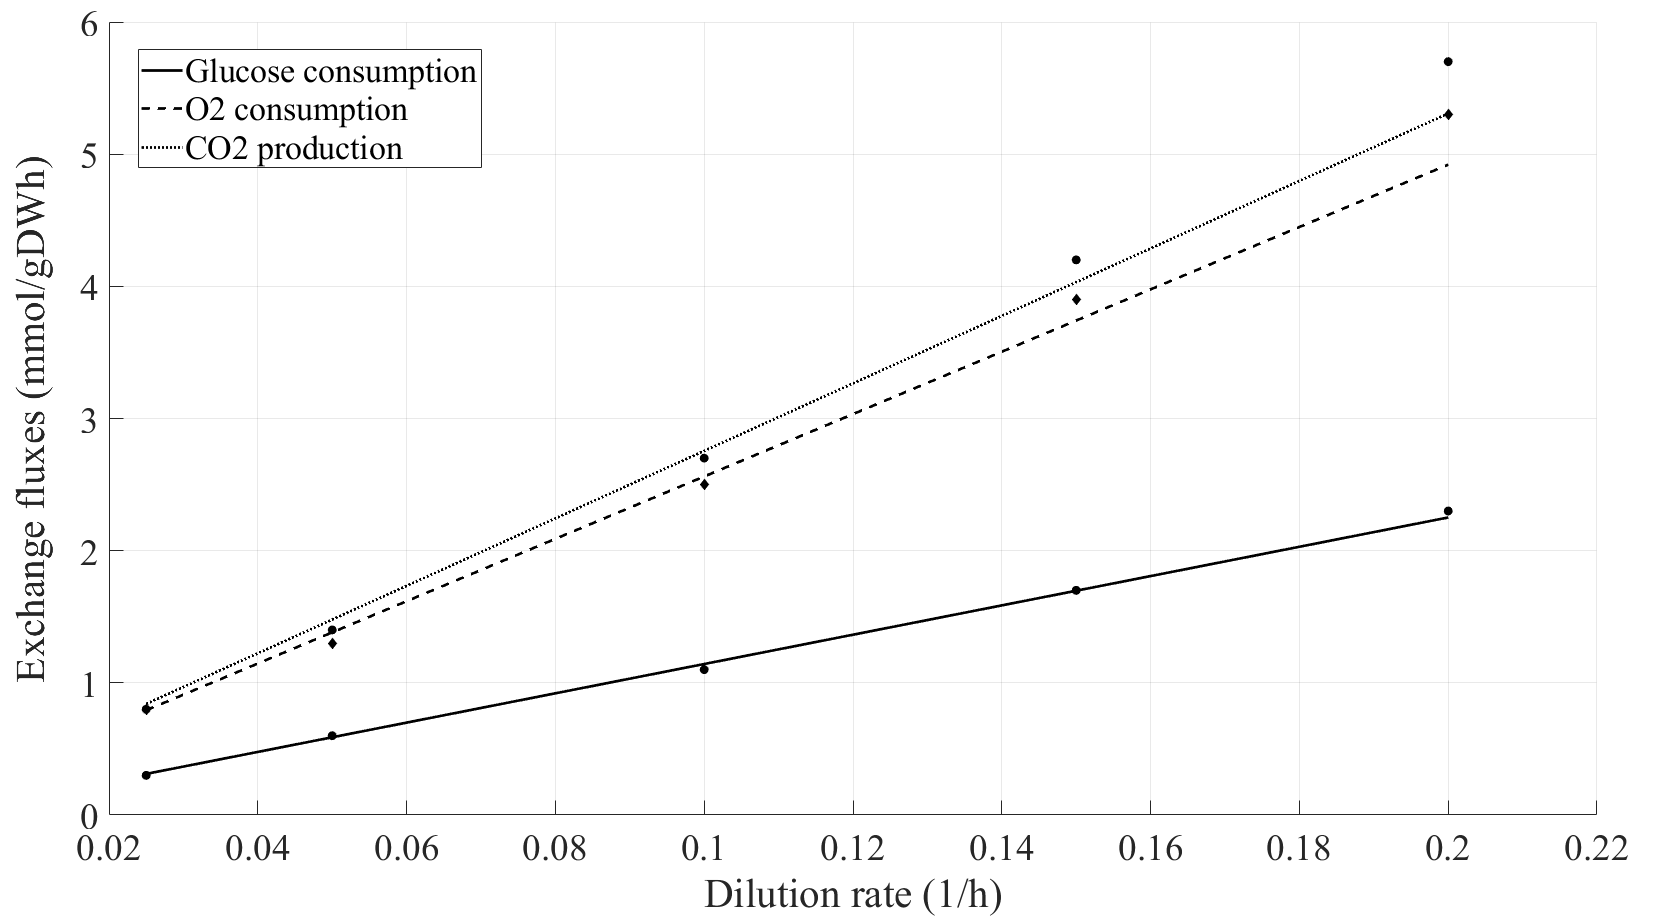
\includegraphics[width=1\columnwidth]{figures/gamfitting.png}
      \caption[The required flux for the growth associated maintenance reaction is determined by the fitting simulation results to the experimental data]{The required flux for the growth associated maintenance reaction is determined by the fitting simulation results to the experimental data. The best fit is found at 31.4 mmol/gDWh\textsuperscript{-1} and the reaction is constrained to that flux value.}
      \label{fig:gam_fitting}
  \end{center}
\end{figure}

Average enzyme saturation value is set to 50\% where the lowest error rate is obtained as a fraction to biomass (Figure \ref{fig:sigma_fitting}). By constraining the total enzyme mass, the metabolic model became able to show overflow metabolism without any other constaint applied.

\begin{figure}[H]
  \begin{center}
    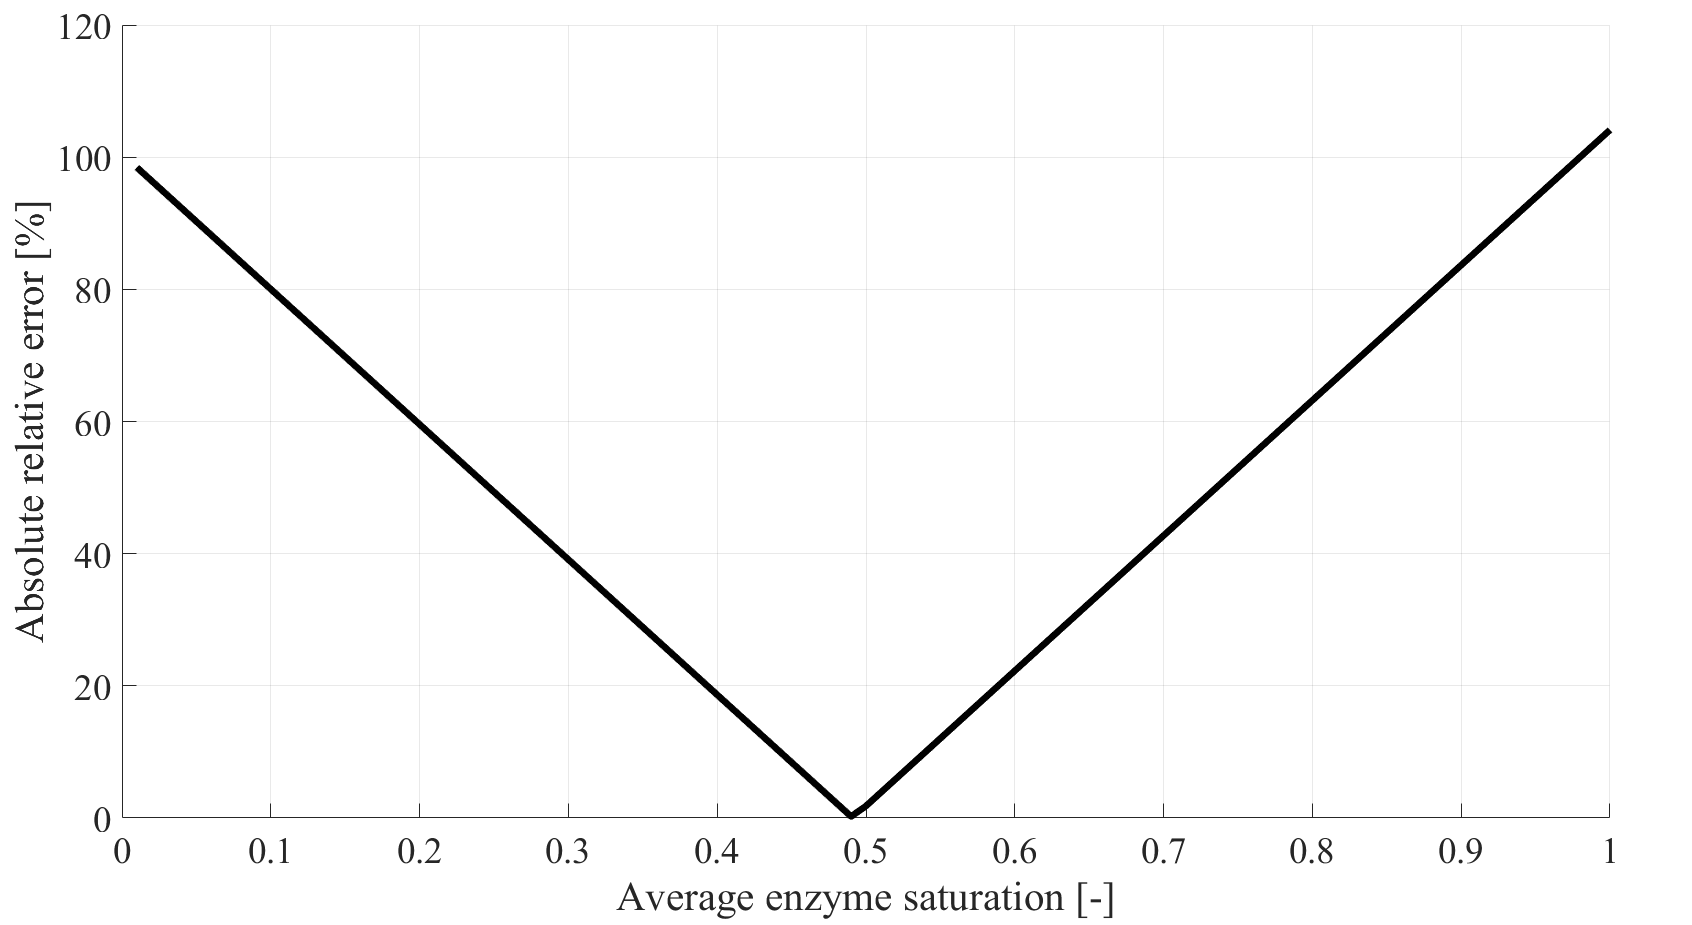
\includegraphics[width=1\columnwidth]{figures/sigmafitting.png}
    \caption[Average enzyme saturation factor for the GECKO method is determined by the iterative simulations for the lowest absolute relative error to the experimantal data]{Average enzyme saturation factor for the GECKO method is determined by the iterative simulations for the lowest absolute relative error to the experimantal data. The value is set to 50\% where the lowest error rate is obtained.}
    \label{fig:sigma_fitting}
  \end{center}
\end{figure}

To prevent over-constraining the model with the enzyme kinetics, the most limiting proteins in the model are found based on their sensitivity on the objective function, i.e. growth. The $k_{cat}$ values for the the limiting enzymes are updated with the maximum available values from BRENDA\cite{jeske2019brenda} database by automated iterations until the simulation results for the growth rate agrees with the experimental growth rate. Modifications to the $k_{cat}$ values with their objective control coefficients can be found in the Table \ref{table:gecko_iterations}.

\begin{table}[H]
  \begin{center}
  \caption[Iterations on the network to find the top limiting proteins by their objective control coefficients (cc), i.e. sensitivities on the growth, with previous and updated $k_{cat}$ values and error improvements]{Iterations on the network to find the top limiting proteins by their objective control coefficients (cc), i.e. sensitivities on the growth, with previous and updated $k_{cat}$ values and error improvements. }
  \vskip0.5\baselineskip
  \begin{tabular}{ccp{5cm}cccc}
     \hline
    \textbf{\#} & \textbf{Protein} & \textbf{Reaction Name} & \textbf{prev $k_{cat}$} & \textbf{new $k_{cat}$} & \textbf{CC} & \textbf{Err\%}  \\
      \hline
      1 & P38604 & lanosterol synthase & 0.002 & 4.076 & 0.937 & -42.6 \\ \hline
      2 & P38972 & 5'-phosphoribosylformyl \newline glycinamidine synthetase & 0.05 & 5.07 & 0.244 & -28.7 \\   \hline
      3 & P00931 & tryptophan synthase \newline (indoleglycerol phosphate) & 0.022 & 775.75 & 0.129 & -19.4 \\   \hline
      4 & P48445 & acetyl-CoA carboxylase & 1.23 & 450000 & 0.065 & -14.2 \\   \hline
      5 & P05694 & methionine synthase & 0.33 & 3.5 & 0.050 & -10.3 \\   \hline
      6 & P39006 & PS decarboxylase \newline (1-16:1, 2-16:1) & 0.053 & 366.667 & 0.043 & -6.4 \\   \hline
  \end{tabular}
  \label{table:gecko_iterations}
  \end{center}
\end{table}


\vspace{-0.5cm}
\section{Differential Expression Analysis and Integration}

The obtained expression datasets were quantile-normalized for their own experiments. Three replicates for both reference and the evolved strains for each experiment (exception with the ethanol-b8 strain which has two replicates) is used for the differential expression analysis. The distribution across normalized gene expression levels across each experiment can be seen in the Figure \ref{fig:expr_boxplot}. No further normalization applied to prevent introducing errors and datasets are used as obtained from the database.

\begin{figure}[H]
  \begin{center}
  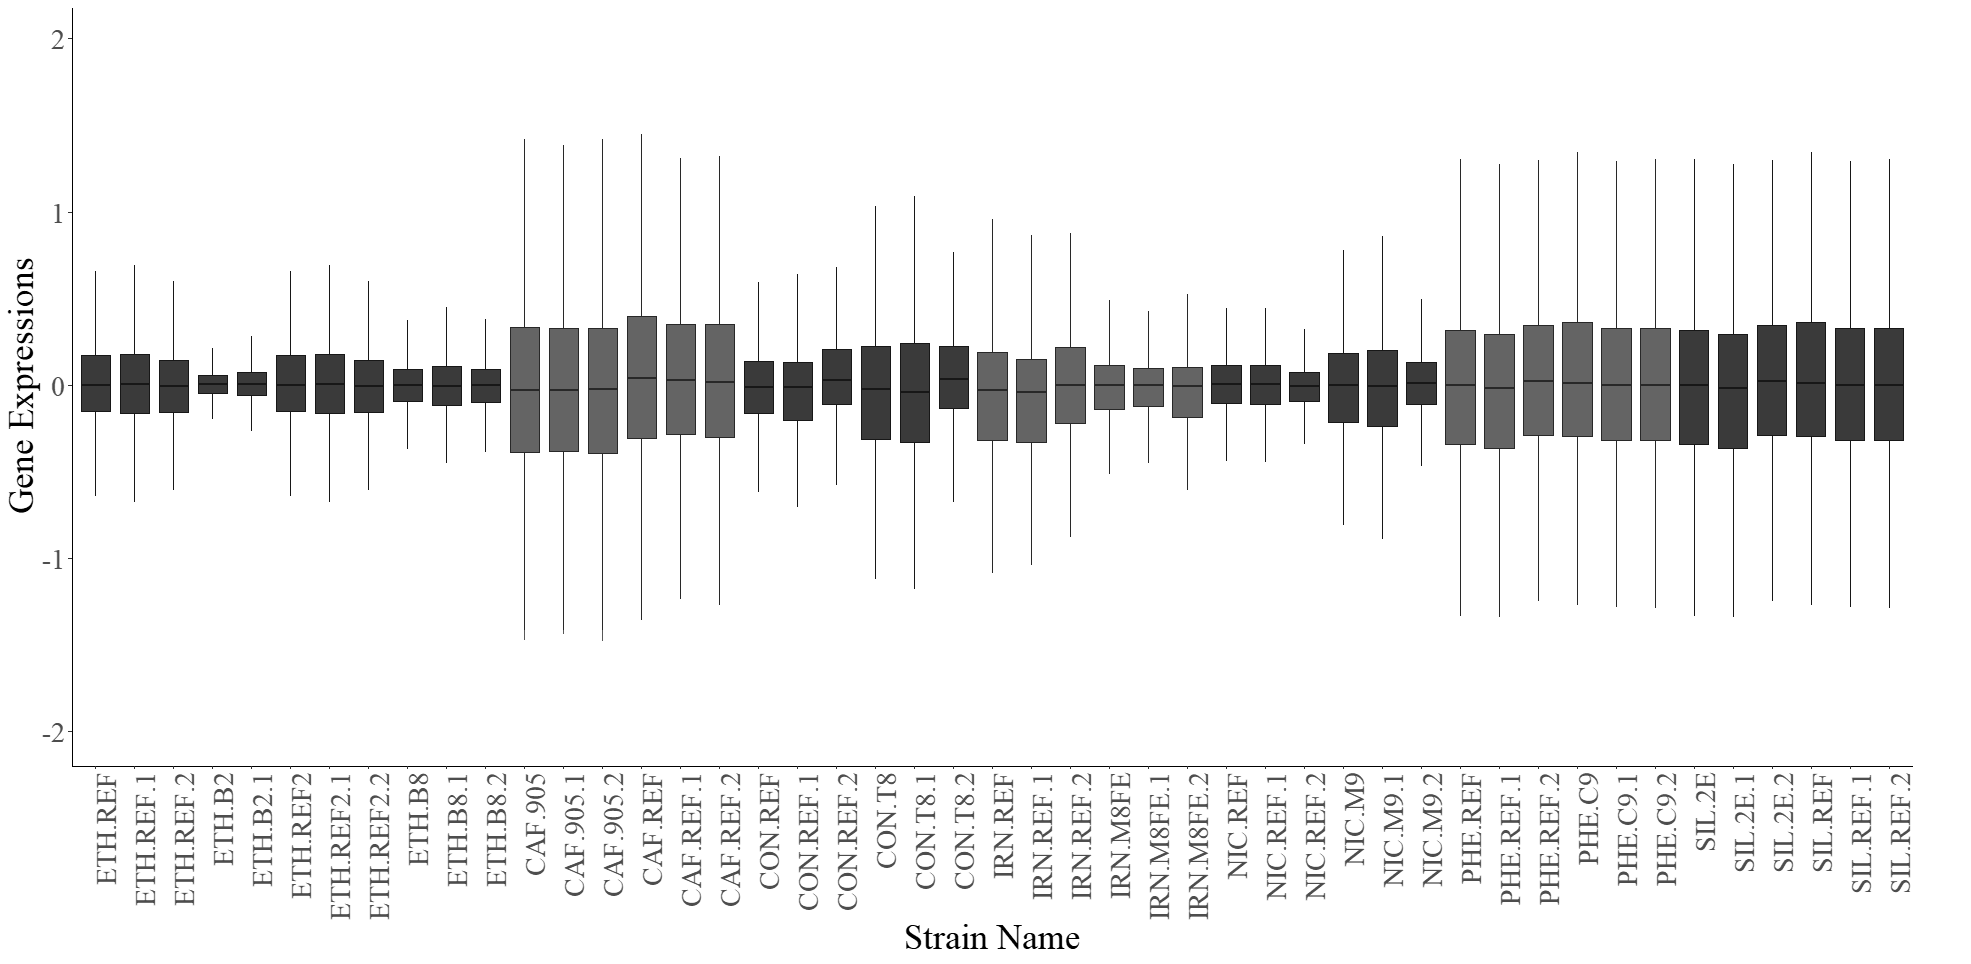
\includegraphics[width=1\columnwidth]{figures/expr_boxplots.png}
  \caption[Boxplots of the normalized gene expression levels]{Boxplots of the normalized gene expression levels obtained from Gene Expression Omnibus. Quantile normalization performance is indicated by the medians (black horizontal lines) that are almost at the same level with their reference reads.}
  \label{fig:expr_boxplot}
  \end{center}
\end{figure}

A statistical threshold (p $<$ 0.05) for the differential analysis of the normalized gene expression levels detected a total of 1606 genes in ethanol-b2, 2947 genes in ethanol-b8, 4743 genes in caffeine, 2267 genes in coniferylaldehyde, 3448 genes in iron, 152 genes in nickel, 4796 genes in phenylethanol, and 4796 genes in silver resistant strains differentially expressed. Commonly upregulated and downregulated genes frequencies across all strains can be found in the Figure \ref{fig:intersections_by_degree}.



\begin{figure}[H]
  \begin{center}
  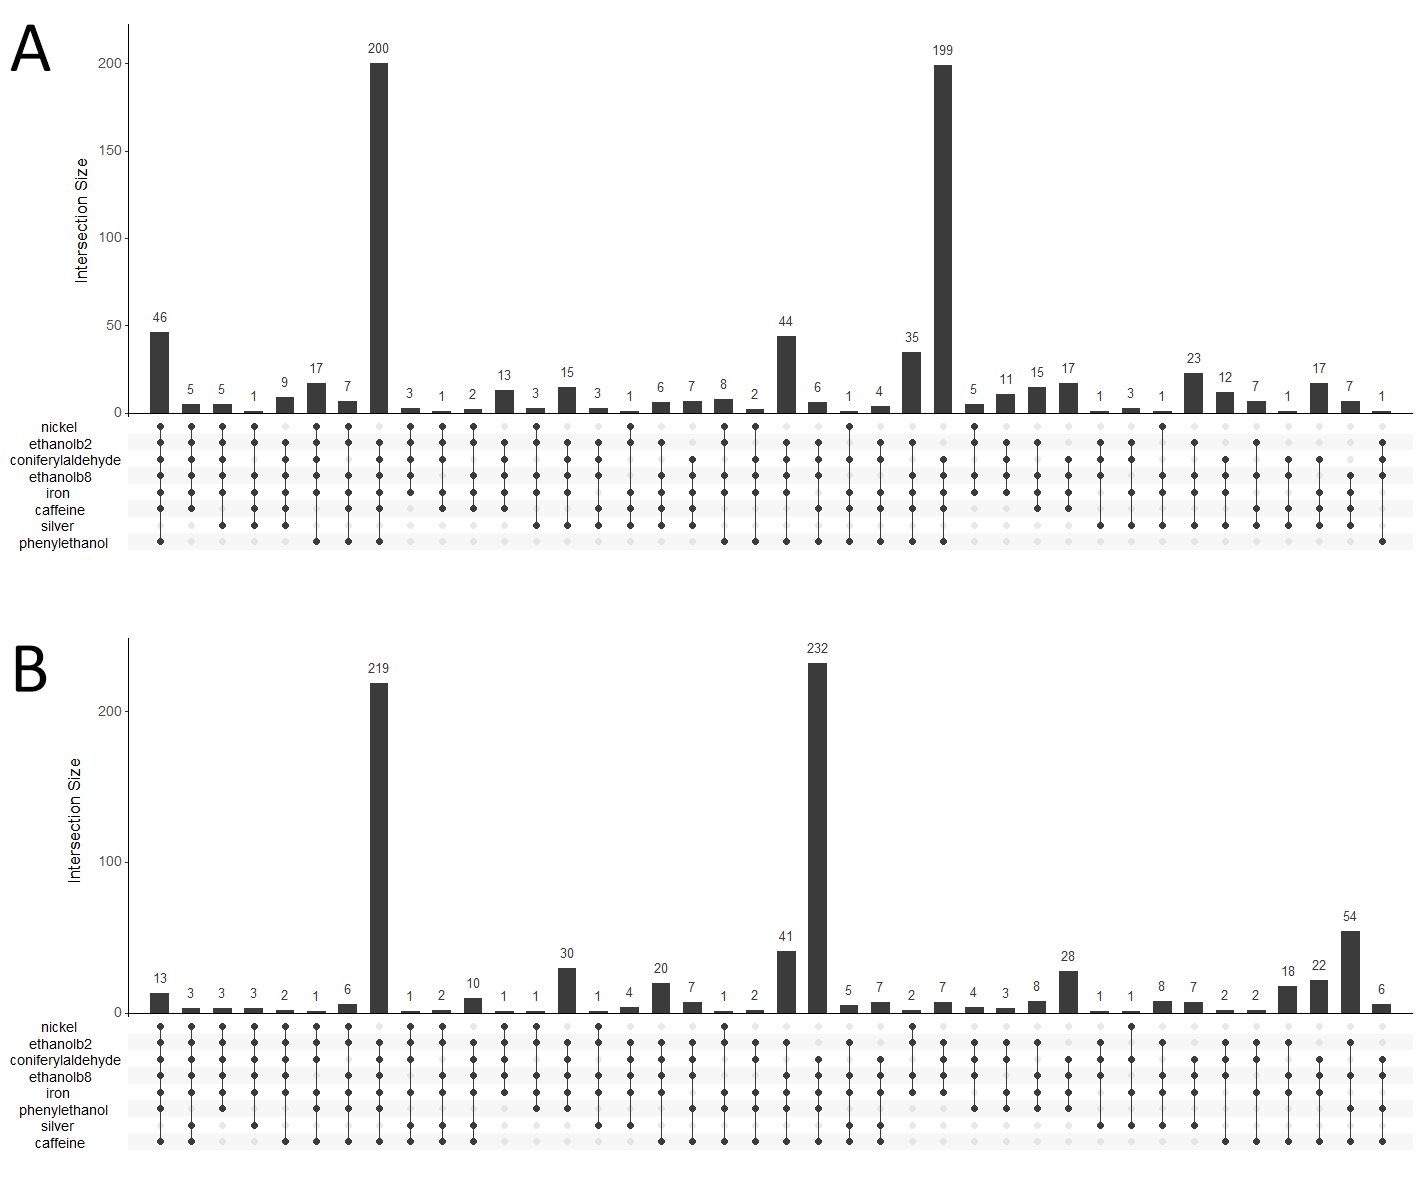
\includegraphics[width=1\columnwidth]{figures/intersections_by_degree.png}
  \caption[UpSet plot showing the number of common genes that are differentially expressed significantly]{UpSet plot showing the number of common genes that are differentially expressed significantly (p $<$ 0.05) across evolved strains. Connected black circles in the below panel's matrix represents a certain intersection between experiment strains, and the number of genes in that intersection are shown in the top bar graphs. Differentially expressed genes are plotted seperately for (A) upregulated genes, and (B) downregulated genes.}
  \label{fig:intersections_by_degree}
  \end{center}
\end{figure}

Despite the high number of differentially expressed genes in the silver resistant strain, the intersection with the most number of strains discluded it. There were not any common differentially expresssed genes considering all strains. The most common genes (as shown in the first bars in the UpSet plot) are reported in Table \ref{table:common_genes}.

\begin{table}[H]
\small
\vskip\baselineskip
  \begin{center}
  \caption[Common upregulated and downregulated genes]{The common upregulated and downregulated genes within ethanolb2, ethanolb8, caffeine, coniferylaldehyde, iron, nickel and phenylethanol resistant strains.}
    \vspace{5mm}
  \begin{tabular}{|p{4cm}|p{10cm}|}
     \hline
    \textbf{Upregulated Genes} & \textbf{Downregulated Genes}  \\
      \hline
      YDR075W, YDR492W, YGR239C, YIL118W, YLR215C, YML005W, YML125C, YNL024C, YNL188W, YNR044W, YOL002C, YOR107W, YPR052C & YBL015W, YBR132C, YBR285W, YBR299W, YCR068W, YDL238C, YDR055W, YER033C, YGL146C, YGL250W, YGR023W, YGR149W, YGR161C, YGR288W, YGR289C, YGR292W, YIL097W, YIR017C, YJL042W, YJL053W, YJL082W, YJL132W, YLR092W, YLR176C, YLR240W, YLR446W, YMR052C-A, YMR053C, YMR081C, YMR103C, YMR104C, YMR105C, YMR160W, YMR194C-A, YMR258C, YMR291W, YNL093W, YNL277W, YNR001C, YOL117W, YOR027W, YOR132W, YOR178C, YOR230W, YPR079W, YPR154W \\ \hline
  \end{tabular}

  \label{table:common_genes}
  \end{center}
\end{table}



The log2(fold-change) values of differentially expressed genes and their frequencies are plotted for each experiment in Figure \ref{fig:expr_frequencies_before}. Although the high number of differentially expressed genes are collected, due to the limited reaction number in the genome-scale metabolic models, only a part of obtained fold-change expression values were able to integrated into the models. Because of the limitations in the model, no further cutoff considered for the fold change values.

\begin{figure}[H]
  \begin{center}
  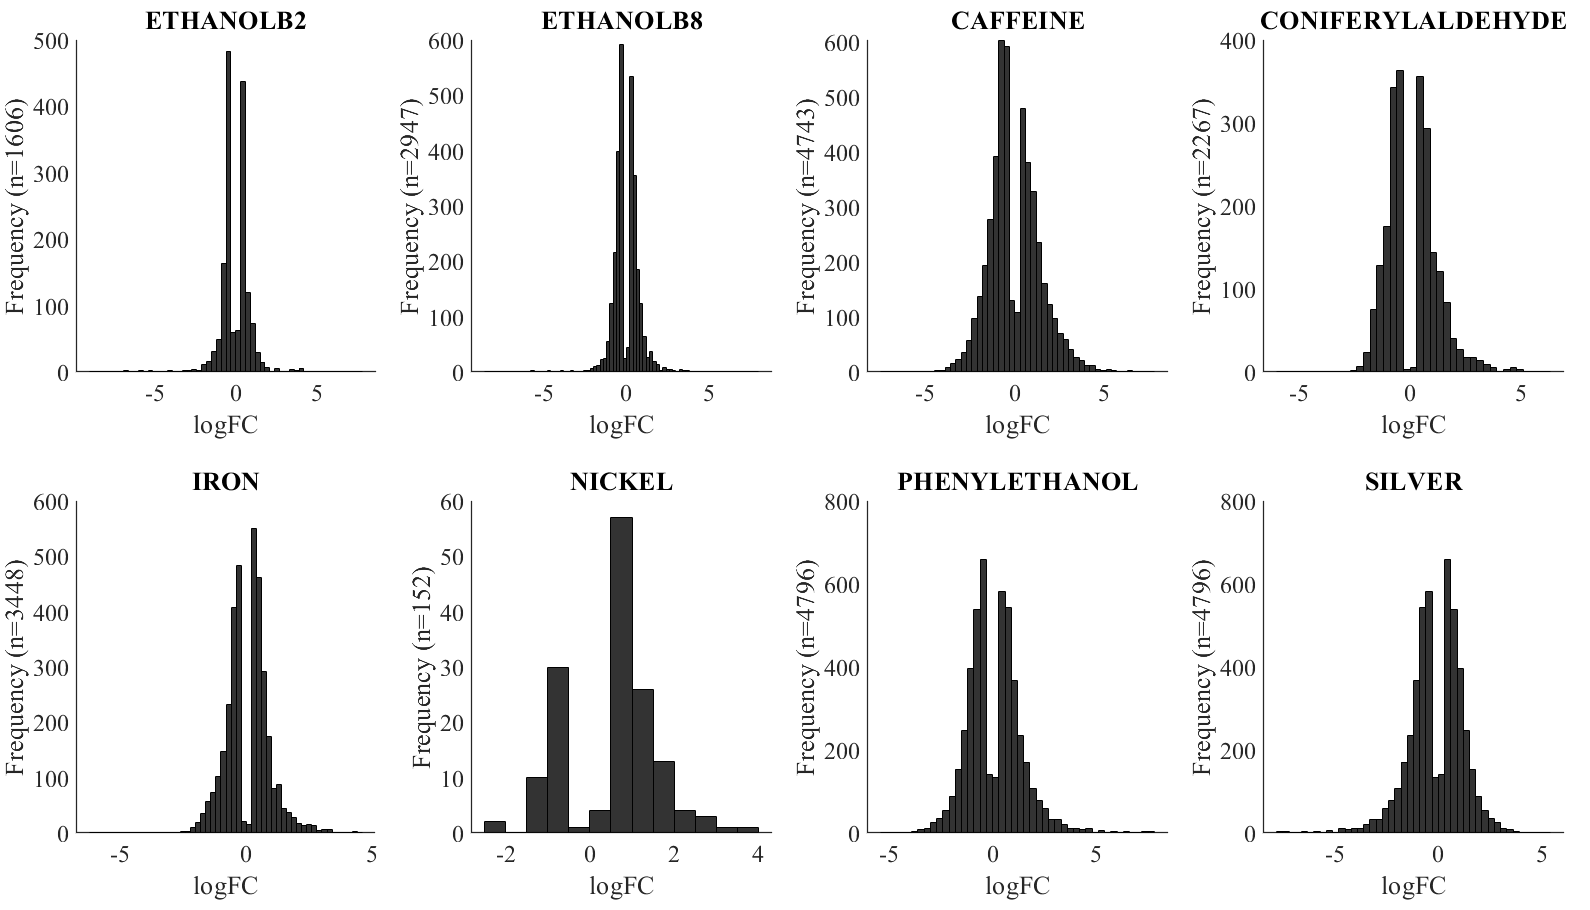
\includegraphics[width=1\columnwidth]{figures/expr_frequencies_before.png}
  \caption[Frequencies of the differentially expressed genes after the gene expression analysis]{Frequencies of the differentially expressed genes after the gene expression analysis.}
  \label{fig:expr_frequencies_before}
  \end{center}
\end{figure}

Total of 277 genes in ethanol-b2, 464 genes in ethanol-b8, 783 genes in caffeine, 374 genes in coniferylaldehyde, 552 genes in iron, 28 genes in nickel, 759 genes in phenylethanol and 759 genes in silver resistant strains were integrated into the metabolic model to generate strain-specific models (\ref{fig:expr_frequencies_after}).

\begin{figure}[H]
  \begin{center}
  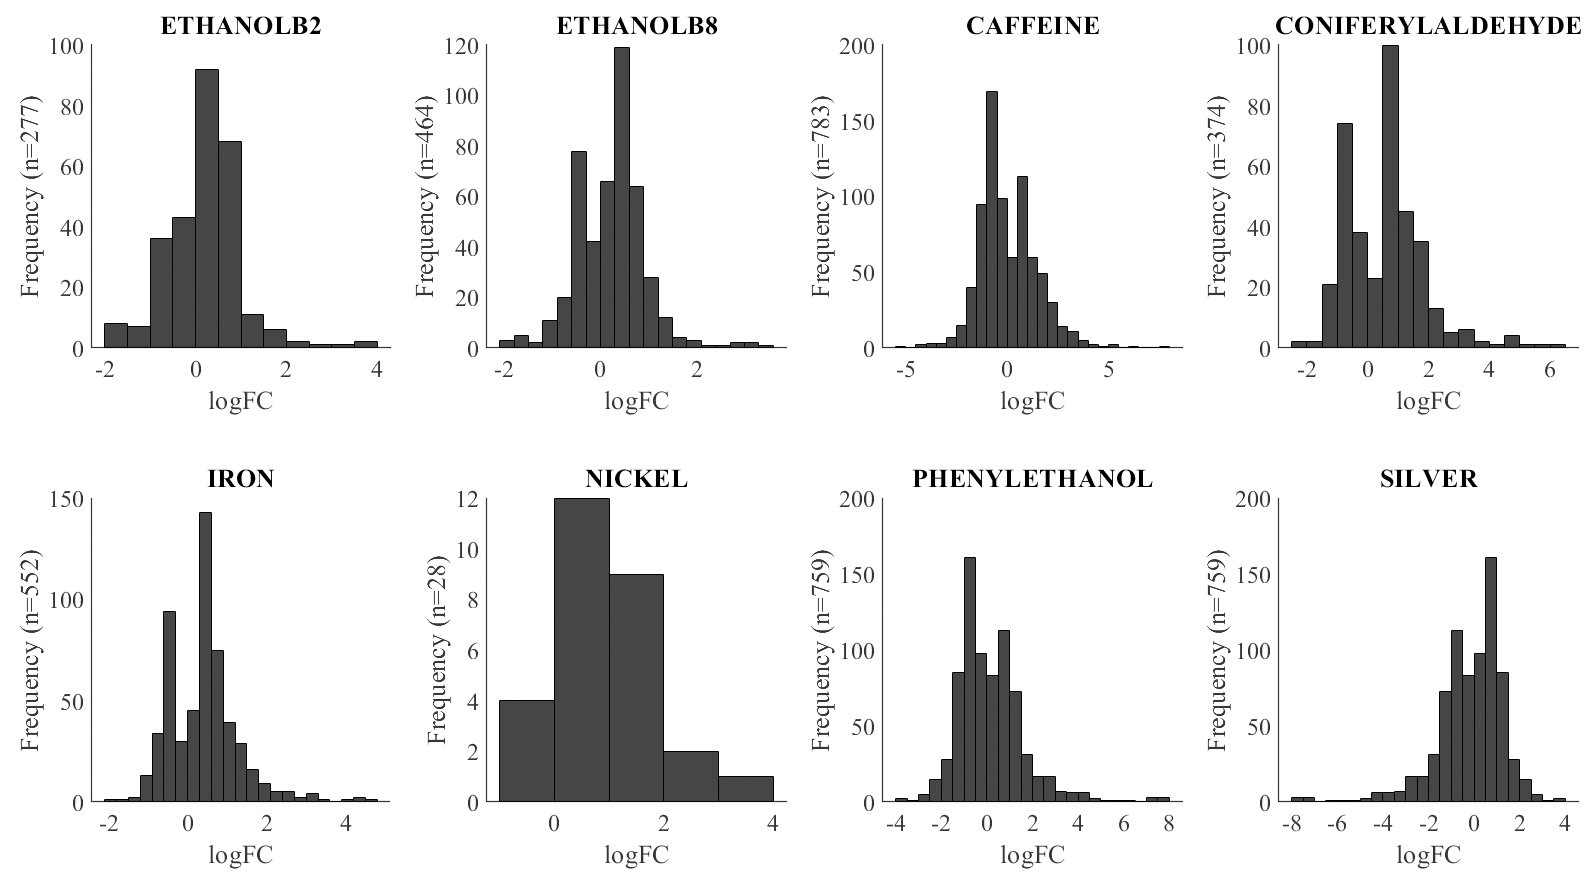
\includegraphics[width=1\columnwidth]{figures/expr_frequencies_after.png}
  \caption[Frequencies of the differentially expressed genes that are integrated into the metabolic model]{Frequencies of the differentially expressed genes that are integrated into the metabolic model.}
  \label{fig:expr_frequencies_after}
  \end{center}
\end{figure}

In order to validate the expression data integration method, fluxes for each enzyme (i.e. protein flux from protein pool to reaction for each protein) is predicted by flux balance analysis on all the strain models and on the wild-type model (wild-type here is referred as the metabolic model without expression data integrated). Flux ratios between wild-type and evolved models are calculated, and linear regression analysis is fitted after elimination of the outliers by the generalized extreme studentized deviate test to compare the flux-changes with the protein fold-changes from the expression data. Results confirm a good correlation between simulations and protein fold-change values (Figure \ref{fig:expr_linear_regressions}).

\begin{figure}[H]
  \begin{center}
  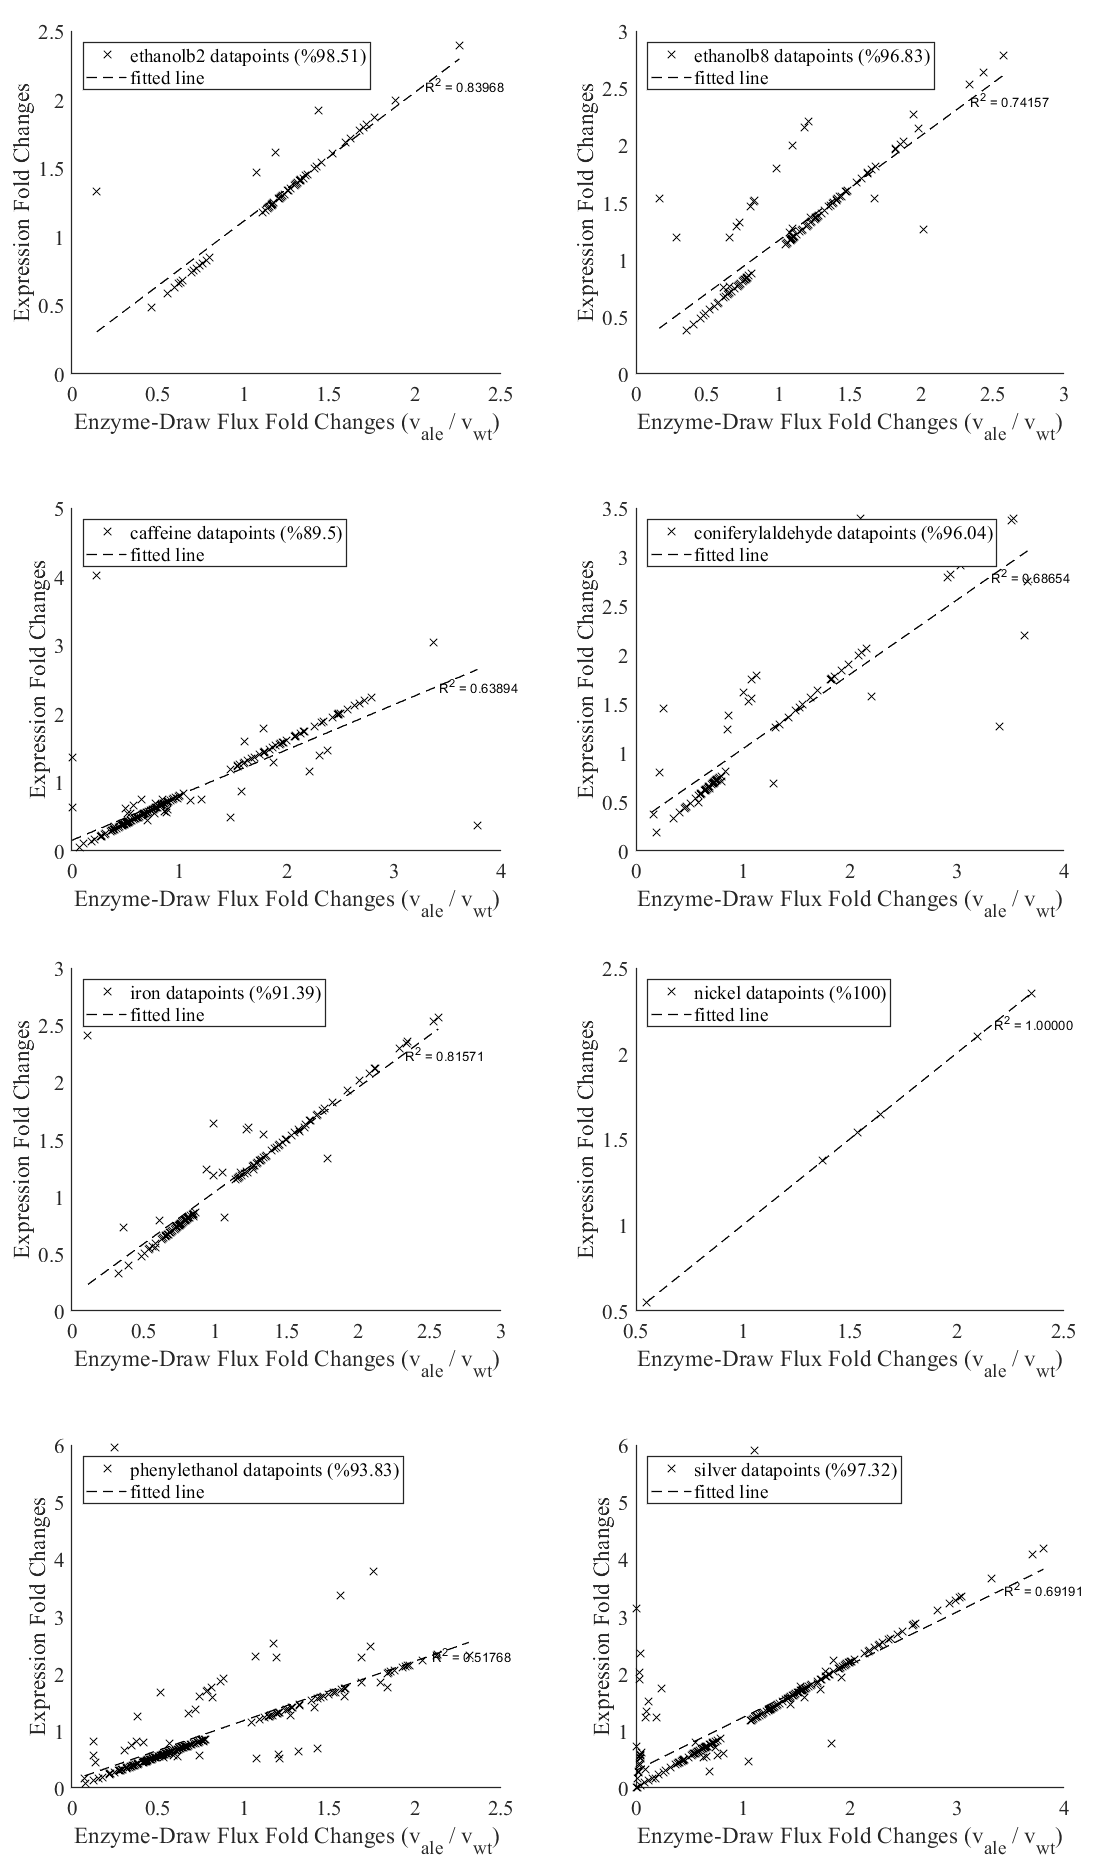
\includegraphics[width=0.8\columnwidth]{figures/expr_linear_regressions.png}
  \caption[Linear regression analyses of the fold-changes]{Linear regression analyses of the differential expression fold-changes obtained from microarray studies and the enzyme-draw flux fold-changes obtained from flux balance analysis simulations of corresponding proteins.}
  \label{fig:expr_linear_regressions}
  \end{center}
\end{figure}



\section{Flux Balance Analysis Simulations}

The metabolic model is first simulated without the integration of the expression data (this model will be referred as wild-type model). Since the model is already enzymatically constrained, the only additional constraint required is the total amout of enzymes available in the enzyme pool. All the lower bounds for reactions were set to 0, and the upper bounds were set to 1000, except for the enzyme pool reaction. By doing that, the model was set free to be able to allocate enzymes as the reactions require. Flux rates of several exchange reactions as a function of growth rate are plotted in Figure \ref{fig:wt_crabtree}.

A behavioral change is observed around the time when growth rate is approximately 0.3 h\textsuperscript{-1}. Since the model is simulated under fully areobic conditions (no constraints applied) and produces ethanol, this behavior can be explained by the Crabtree effect, where the yeast metabolism switches to perform both respiration and fermantation at the same time at a critical specific growth rate.

\begin{figure}[H]
  \begin{center}
  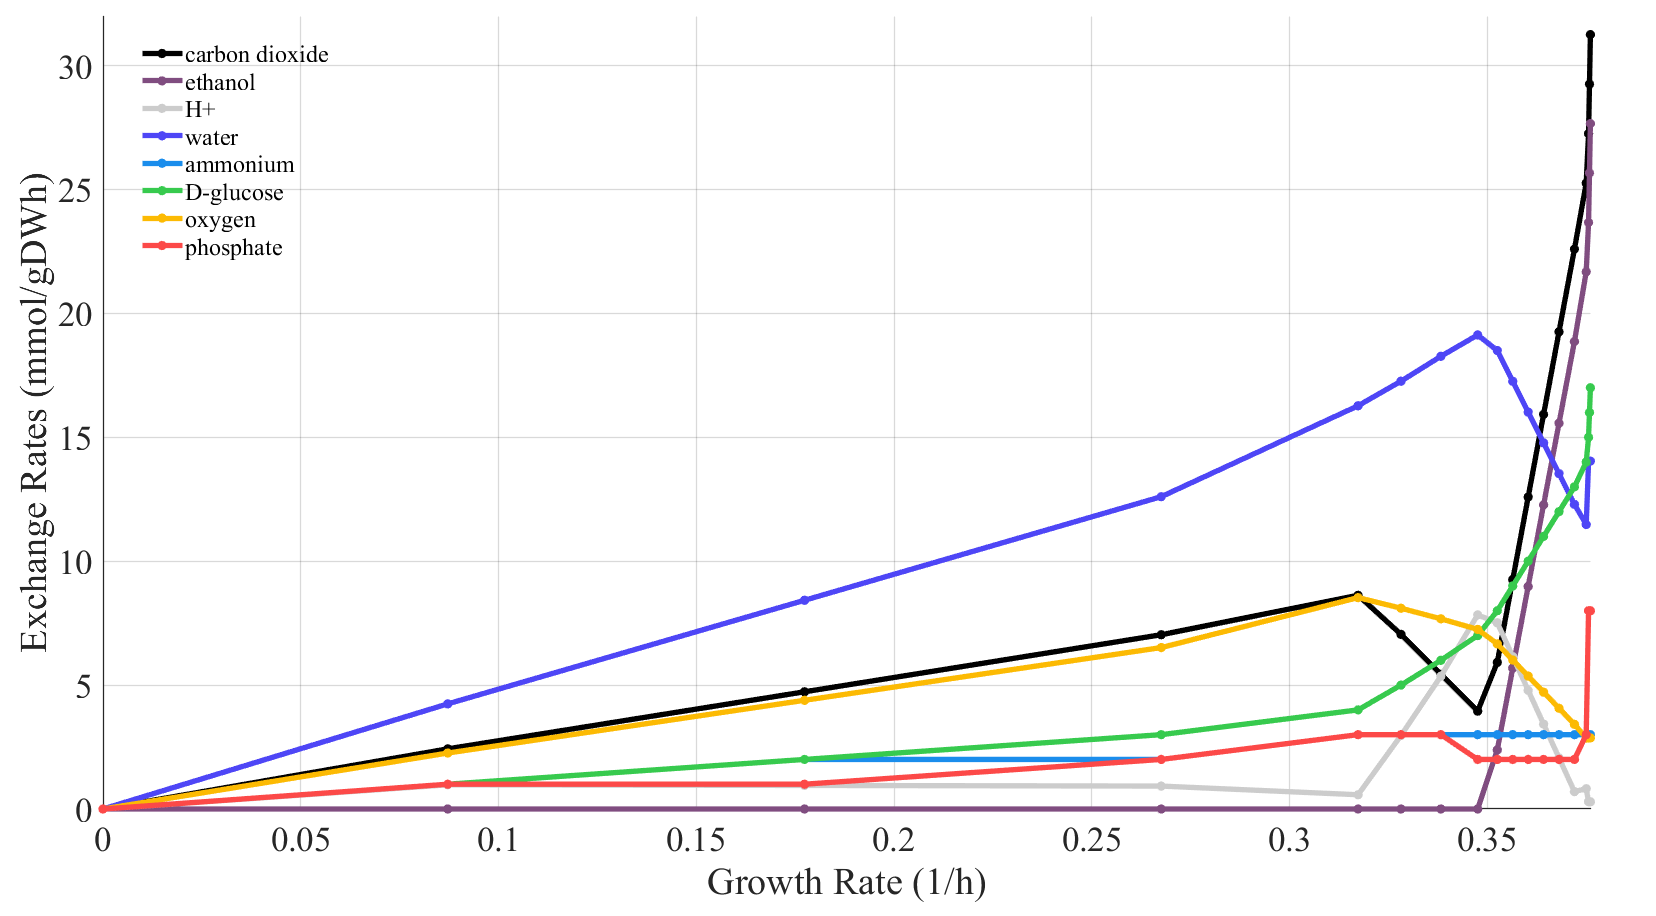
\includegraphics[width=1\columnwidth]{figures/wt_crabtree.png}
  \caption[Metabolic model shows the overflow metabolism]{Metabolic model shows the overflow metabolism (crabtree effect) under fully aerobic conditions.}
  \label{fig:wt_crabtree}
  \end{center}
\end{figure}

Robustness analysis is performed on the wild-type model for the growth rate with the varying levels of glucose uptake, oxygen uptake, acetate secretion and ethanol secretion rates (Figure \ref{fig:wt_robustness}). Unlike the traditional metabolic models, enzymatically constrained model showed non-linear graphs.

\begin{figure}[H]
  \begin{center}
  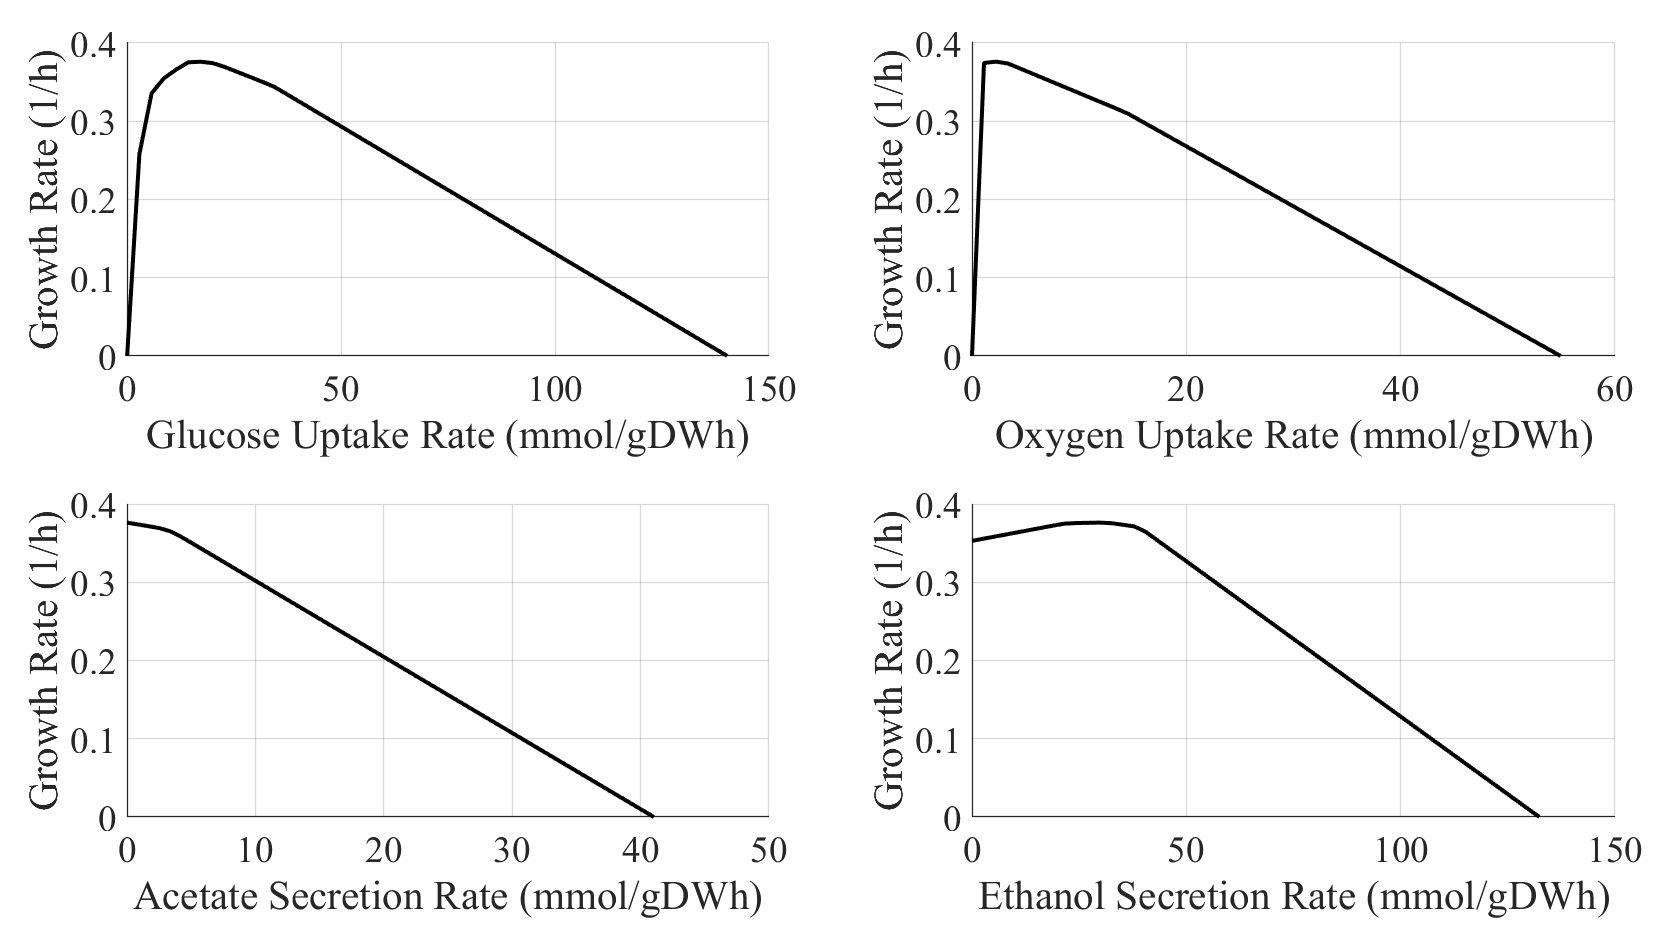
\includegraphics[width=1\columnwidth]{figures/wt_robustness.png}
  \caption[Robustness analyses on the glucose uptake, oxygen uptake, acetate secretion and ethanol secretion rates]{Robustness analyses on the glucose uptake, oxygen uptake, acetate secretion and ethanol secretion rates.}
  \label{fig:wt_robustness}
  \end{center}
\end{figure}

After the validation of the wild-type model, all models for strains are simulated for the growth rates as a function of iteratively increasing glucose uptake rates (Figure \ref{fig:growth_glucose_ales}). Models were able to grow up to the point where the protein accesibility becomes a limiting factor. It has been found that the evolution models except for the caffeine tolerant model show similar patterns on the points where the enzymes become limiting (break points in the lines). Caffeine tolerant model shows different pattern in a way that it can consume more glucose to reach higher growth rates compared to others. Also it must be noted that while only caffeine and coniferylaldehyde tolerant models can grow at higher rates than wild-type model, ethanol, iron, nickel, phenylethanol and silver models can grow at lower maximum rates. The maximum growth rates and corresponding glucose uptake rates for each model are summarized in the Table \ref{table:growth_glucose_table}.

\begin{figure}[H]
  \begin{center}
  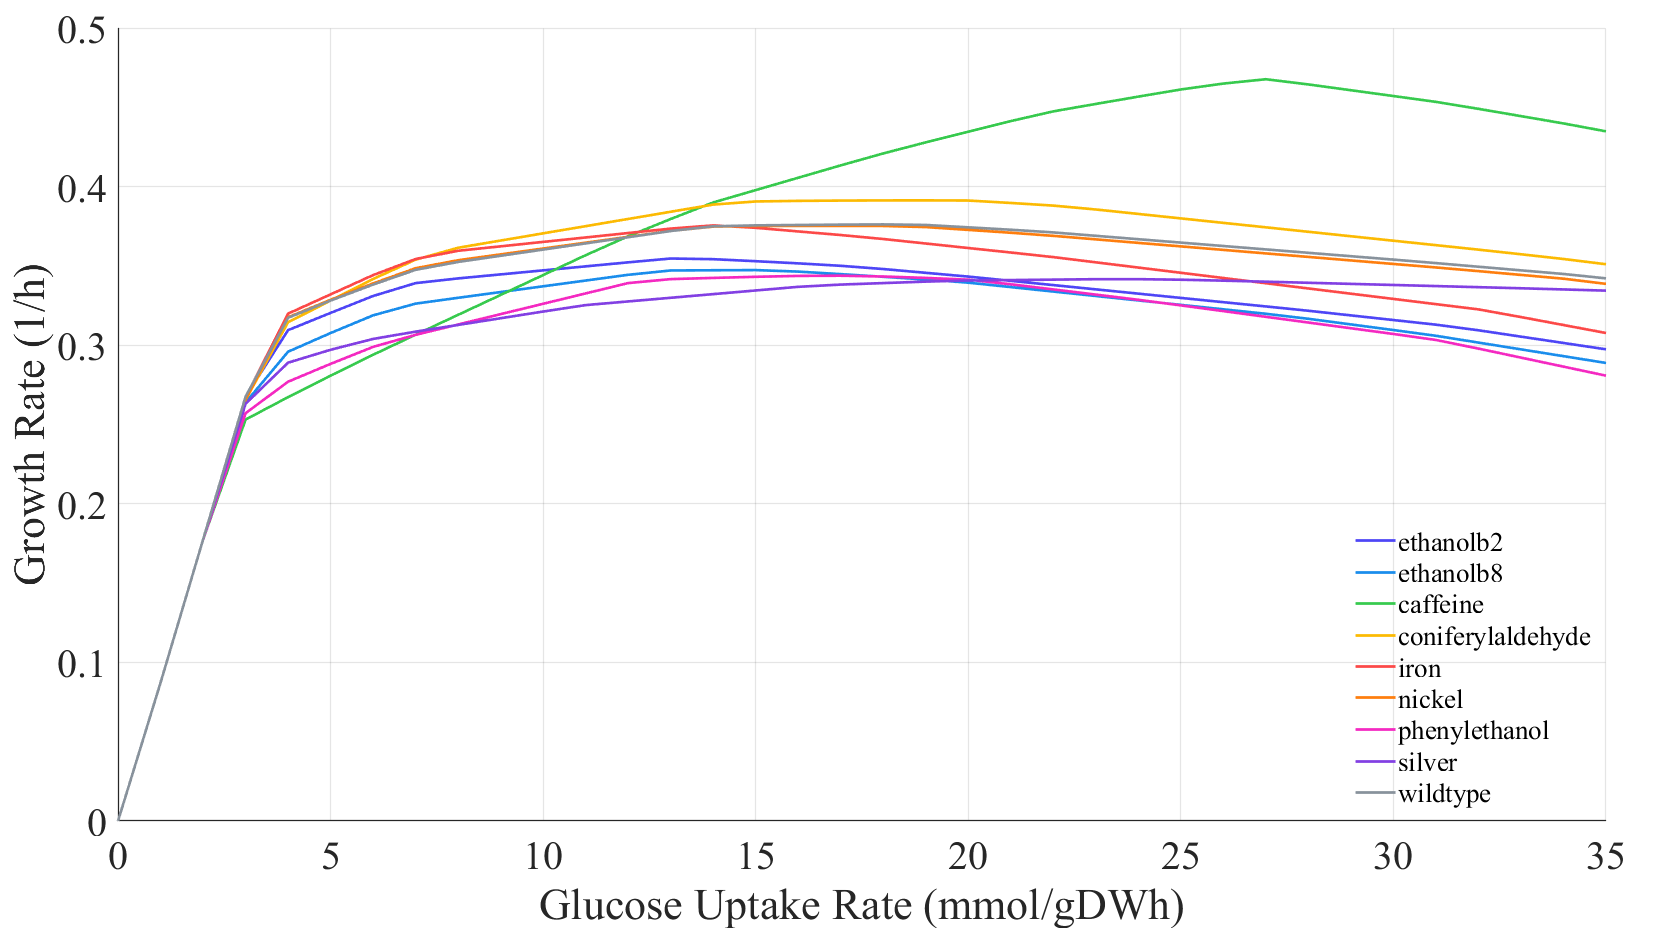
\includegraphics[width=1\columnwidth]{figures/growth_glucose_ales.png}
  \caption[Growth rates as a function of iteratively increasing glucose uptake rates]{Growth rates as a function of iteratively increasing glucose uptake rates.}
  \end{center}
  \label{fig:growth_glucose_ales}
  \end{figure}
\vspace{-1.0cm}



\begin{table}[H]
\small
\vskip\baselineskip
  \begin{center}
  \caption[Maximum growth rates obtained from flux balance analysis simulations for each strain and their maximum glucose uptake rates (GUR) required for the growth]{Maximum growth rates obtained from flux balance analysis simulations for each strain and their maximum glucose uptake rates (GUR) required for the growth.}
    \vspace{5mm}
  \begin{tabular}{|c|c|c|}
     \hline
    \textbf{Experiment} & \textbf{Growth Rate (1/h)} & \textbf{GUR (mmol/gDWh)} \\
      \hline
      ethanolb2           & 0.35466                    & 14                                       \\ \hline
      ethanolb8           & 0.34736                    & 16                                       \\ \hline
      caffeine            & 0.46769                    & 28                                       \\ \hline
      coniferylaldehyde   & 0.39132                    & 20                                       \\ \hline
      iron                & 0.37554                    & 15                                       \\ \hline
      nickel              & 0.37523                    & 18                                       \\ \hline
      phenylethanol       & 0.34382                    & 18                                       \\ \hline
      silver              & 0.34163                    & 25                                       \\ \hline
      wildtype            & 0.37618                    & 19                                       \\ \hline
  \end{tabular}

  \label{table:growth_glucose_table}
  \end{center}
\end{table}

In order to characterize the differentiating reactions in the flux balance analysis solution vectors, cumulative flux vectors of each experiment are plotted (Figure \ref{fig:cumflux_free}). Standart deviations for each reaction between strains are calculated to find most diverging points and plotted as a bar graph.

\begin{figure}[H]
  \begin{center}
  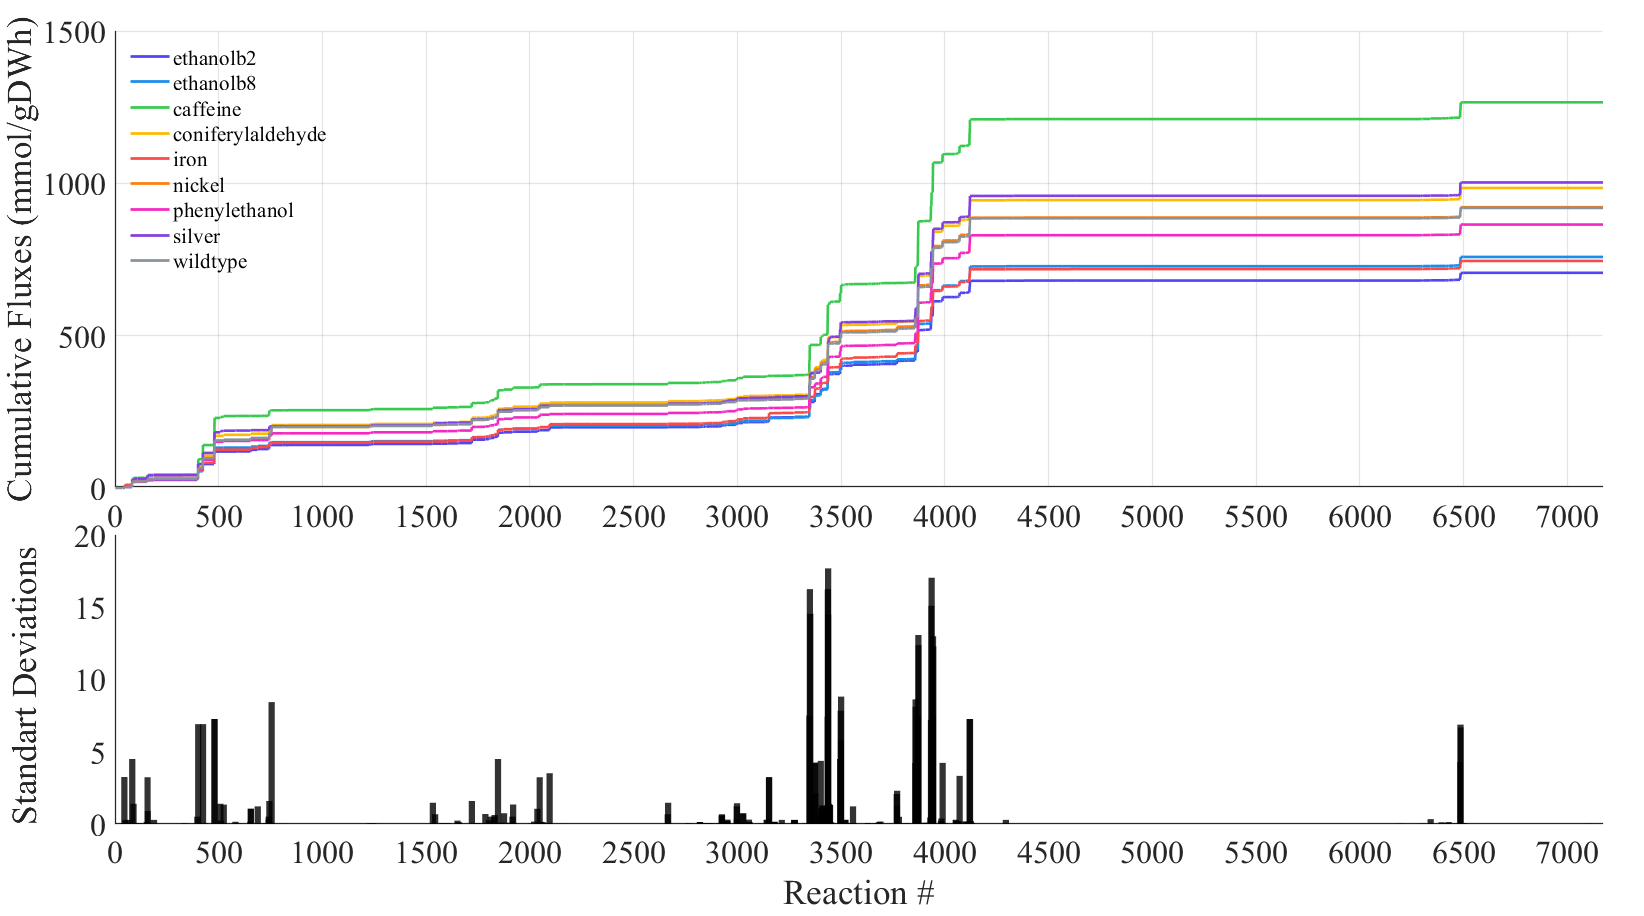
\includegraphics[width=1\columnwidth]{figures/cumflux_free.png}
  \caption[Cumulative flux vectors of each simulation and standart deviations]{Cumulative flux vectors of each model and the standart deviations of reactions across each adaptatoin.}
  \label{fig:cumflux_free}
  \end{center}
\end{figure}

Reactions with the standart deviation values more than 10 mmol/gDWh are listed in Table \ref{table:cumulative_free_stds}. The same reactions with different numbers in their names use different enzymes. For example, glyceraldehyde-3-phosphate dehydrogenase (GADPH) reaction can be carried out in the presence of YGR192C or YJL052W or YJR009C genes' proteins, in other words, TDH1 or TDH2 or TDH3 isozymes. Therefore there are No1, No2 and No3 versions of the same reaction, using different enzymes. It must be noted that these multiple reactions carried out with isozymes in the metabolic model may not mean a significant difference if the enzymes do not catalyze any other reaction. This means that the chosen isozyme may not matter mathematically if the flux value across the isozyme reactions are the same.

\begin{table}[H]
\caption[The most divergent reactions according to their standart deviations across all strains and their flux values in mmol/gDWh.]{The most divergent reactions according to their standart deviations across all strains and their flux values in mmol/gDWh.}
\begin{center}
  \setlength{\tabcolsep}{4pt}
  \resizebox{\textwidth}{!}{
  \begin{tabular}{cclcccccccccc}
\textbf{Rank} & \textbf{Genes} & \textbf{Reaction Nams}                            & \textbf{ethanolb2} & \textbf{ethanolb8} & \textbf{caffeine} & \textbf{coniferylaldehyde} & \textbf{iron} & \textbf{nickel} & \textbf{phenylethanol} & \textbf{silver} & \textbf{wildtype} & \textbf{std} \\ \hline
1             & YJL052W        & glyceraldehyde-3-phosphate  dehydrogenase   (No2) & 24.13              & 0                  & 0                 & 36.82                      & 0             & 32.79           & 0                      & 37.4            & 32.87             & 17.69        \\
2             & YLR134W        & pyruvate decarboxylase (No3)                      & 0                  & 0                  & 44.31             & 0                          & 22.11         & 0               & 30.08                  & 0               & 0                 & 17.04        \\
3             & YGR192C        & glyceraldehyde-3-phosphate  dehydrogenase   (No1) & 0                  & 0                  & 48.77             & 0                          & 0             & 0               & 0                      & 0               & 0                 & 16.26        \\
4             & YGR254W        & enolase (No2)                                     & 23.84              & 0                  & 48.77             & 36.5                       & 25.04         & 32.49           & 32.46                  & 0               & 32.56             & 16.25        \\
5             & YLR044C        & pyruvate decarboxylase (No2)                      & 20.94              & 25.19              & 0                 & 33.69                      & 0             & 29.42           & 0                      & 35.33           & 29.49             & 15.1         \\
6             & YMR323W        & enolase (No4)                                     & 0                  & 28.03              & 0                 & 0                          & 0             & 0               & 0                      & 37.13           & 0                 & 14.55        \\
7             & YJR009C        & glyceraldehyde-3-phosphate  dehydrogenase   (No3) & 0                  & 28.31              & 0                 & 0                          & 25.34         & 0               & 32.74                  & 0               & 0                 & 14.52        \\
8             & YOR283W        & phosphoglycerate mutase (No1)                     & 23.84              & 28.03              & 48.77             & 36.5                       & 25.04         & 32.49           & 32.46                  & 0               & 32.56             & 13.08        \\
9             & YAL038W        & pyruvate kinase (No1)                             & 23.6               & 27.79              & 48.45             & 36.24                      & 24.79         & 32.23           & 32.23                  & 0               & 32.31             & 12.99        \\
10            & YKL152C        & phosphoglycerate mutase (No2)                     & 0                  & 0                  & 0                 & 0                          & 0             & 0               & 0                      & 37.13           & 0                 & 12.38        \\
11            & YOR347C        & pyruvate kinase (No2)                             & 0                  & 0                  & 0                 & 0                          & 0             & 0               & 0                      & 36.9            & 0                 & 12.3
\end{tabular}}
\label{table:cumulative_free_stds}
\end{center}
\end{table}


Cumulative flux vectors of each experiment are plotted once more when the boundaries of the glucose uptake reaction is constrained to 10 gDWh\textsuperscript{-1} for each model (Figure \ref{fig:cumflux_gur10}). This has done to eliminate differences might be arising because of the free glucose uptake rates (as shown in below section, each model can uptake different maximum amount of glucose) and therefore affecting the downstream reaction fluxes.

\begin{figure}[H]
  \begin{center}
  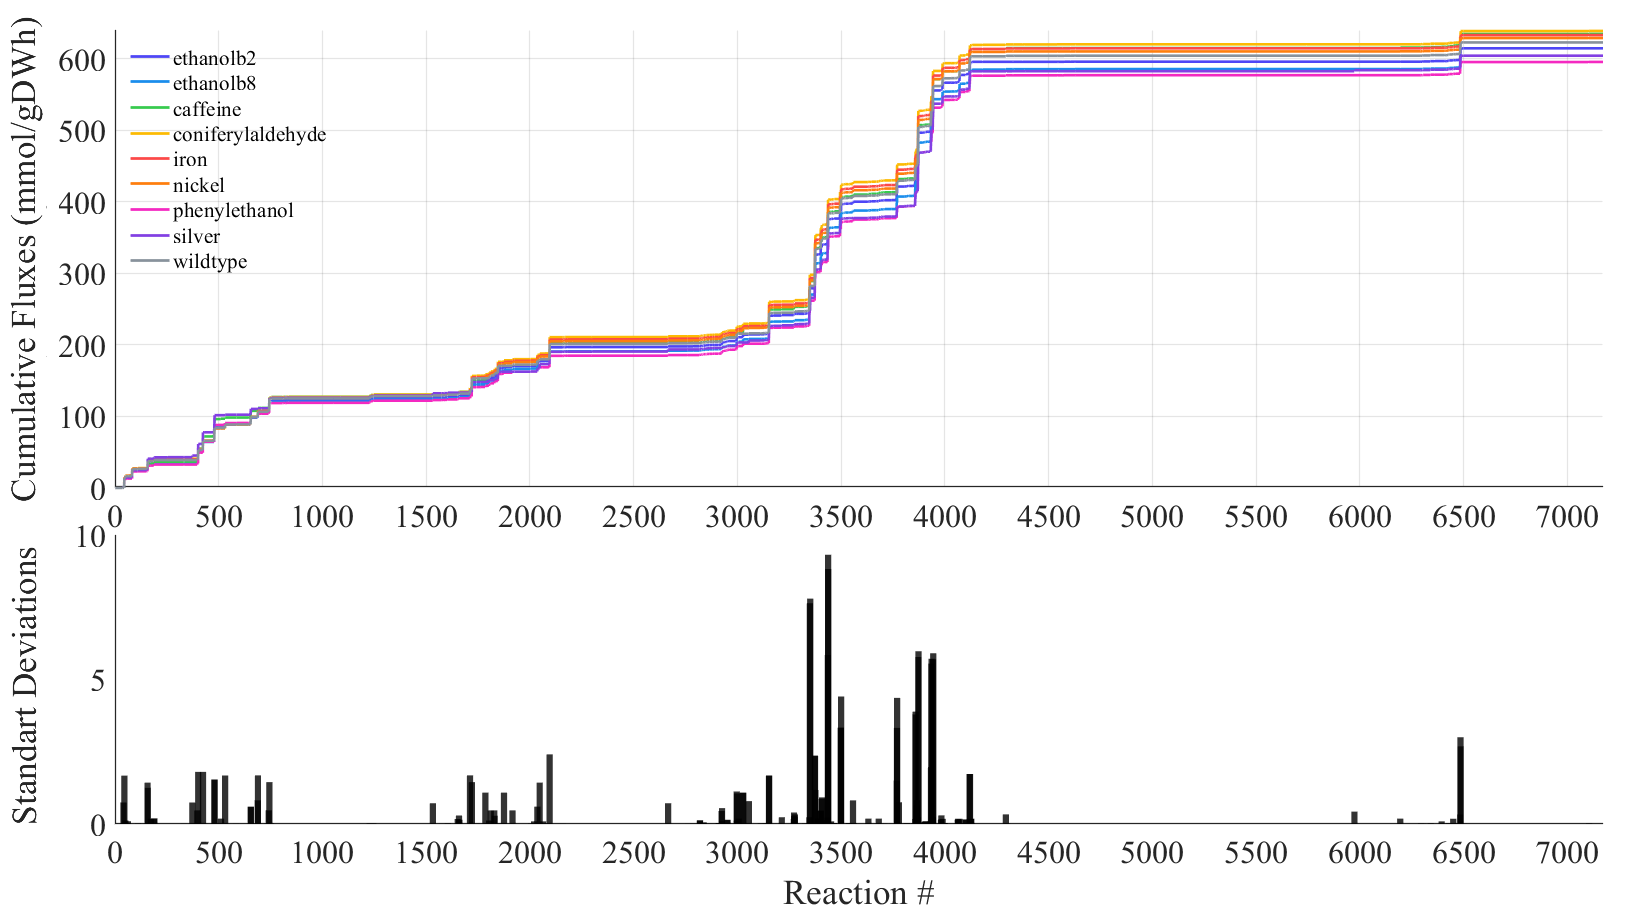
\includegraphics[width=1\columnwidth]{figures/cumflux_gur10.png}
  \caption[Cumulative flux vectors of each experiment when glucose uptake rate is constrained]{Cumulative flux vectors of each simulation and standart deviations. Glucose uptake rate is constrainted to  10 mmol/gDWh for all models. }
  \label{fig:cumflux_gur10}
  \end{center}
\end{figure}

Reactions with the standart deviation values more than 5 mmol/gDWh are listed in Table \ref{table:cumulative_free_stds}. Despite the decrease in the flux values (caused by the lower uptake rates of glucose), the top divergent reactions obtained are in agreement with the no-constraint flux balance analysis results.

\begin{table}[H]
\caption[The most divergent reactions across all strains and their flux values in mmol/gDWh when the glucose uptake rate is constrained to 10 mmol/gDWh.]{The most divergent reactions across all strains and their flux values in mmol/gDWh when the glucose uptake rate is constrained to 10 mmol/gDWh.}
\begin{center}
\setlength{\tabcolsep}{4pt}
\resizebox{\textwidth}{!}{
\begin{tabular}{|c|c|l|c|c|c|c|c|c|c|c|c|c|}
\hline
\textbf{\#} & \textbf{Gene} & \textbf{Reaction Name}                                                                     & \textbf{b2-eth} & \textbf{b8-eth} & \textbf{caff.} & \textbf{con. ald.} & \textbf{iron} & \textbf{nickel} & \textbf{phen.} & \textbf{silver} & \textbf{ref.} & \textbf{std} \\ \hline
1           & TDH1          & \begin{tabular}[c]{@{}l@{}}glyceraldehyde-\\ 3-phosphate \\ dehydrogenase (2)\end{tabular} & 17.64           & 0               & 0              & 17.48              & 0             & 17.54           & 0              & 18.18           & 17.55             & 9.32         \\ \hline
2           & TDH2          & \begin{tabular}[c]{@{}l@{}}glyceraldehyde-\\ 3-phosphate \\ dehydrogenase (3)\end{tabular} & 0               & 17.7            & 0              & 0                  & 17.51         & 0               & 17.71          & 0               & 0                 & 8.82         \\ \hline
4           & ERR3          & enolase (4)                                                                                & 0               & 17.43           & 0              & 0                  & 0             & 0               & 0              & 17.93           & 0                 & 7.8          \\ \hline
5           & ENO1          & enolase (2)                                                                                & 17.36           & 0               & 17.54          & 17.18              & 17.22         & 17.25           & 17.45          & 0               & 17.26             & 7.64         \\ \hline
6           & GPM1          & \begin{tabular}[c]{@{}l@{}}phosphoglycerate \\ mutase (2)\end{tabular}                     & 0               & 0               & 0              & 0                  & 0             & 0               & 0              & 17.93           & 0                 & 5.98         \\ \hline
8           & PYK2          & pyruvate kinase (2)                                                                        & 0               & 0               & 0              & 0                  & 0             & 0               & 0              & 17.72           & 0                 & 5.91         \\ \hline
9           & TDH3          & \begin{tabular}[c]{@{}l@{}}glyceraldehyde-\\ 3-phosphate \\ dehydrogenase (1)\end{tabular} & 0               & 0               & 17.54          & 0                  & 0             & 0               & 0              & 0               & 0                 & 5.85         \\ \hline
10          & YOR283W       & \begin{tabular}[c]{@{}l@{}}phosphoglycerate \\ mutase (1)\end{tabular}                     & 17.36           & 17.43           & 17.54          & 17.18              & 17.22         & 17.25           & 17.45          & 0               & 17.26             & 5.78         \\ \hline
11          & PDC5          & \begin{tabular}[c]{@{}l@{}}pyruvate \\ decarboxylase (3)\end{tabular}                      & 0               & 0               & 12.6           & 0                  & 9.08          & 0               & 12.15          & 0               & 0                 & 5.72         \\ \hline
12          & CDC19         & \begin{tabular}[c]{@{}l@{}}pyruvate \\ kinase (1)\end{tabular}                             & 17.12           & 17.21           & 17.31          & 16.93              & 16.97         & 17.01           & 17.23          & 0               & 17.01             & 5.7          \\ \hline
13          & PDC1          & \begin{tabular}[c]{@{}l@{}}pyruvate \\ decarboxylase (2)\end{tabular}                      & 10.36           & 11.08           & 0              & 8.69               & 0             & 9.37            & 0              & 14.54           & 9.42              & 5.55         \\ \hline
\end{tabular}}
\label{table:cumulative_gur10_stds}
\end{center}
\end{table}


Finally, only arm reactions (where the isozyme reactions are combined, see Methods) when the glucose uptake rate is constrained to 10 mmol/gDWh are plotted as heatmap in Figure \ref{fig:fba_heatmap}. As it can be seen from the previous tables, most of the differences were caused by the isozymes with the flux values close to each other. By considering only arm reactions and a fixed glucose uptake rate, the reactions that are actually differ because of the expression integration are found.

\begin{figure}[H]
  \begin{center}
  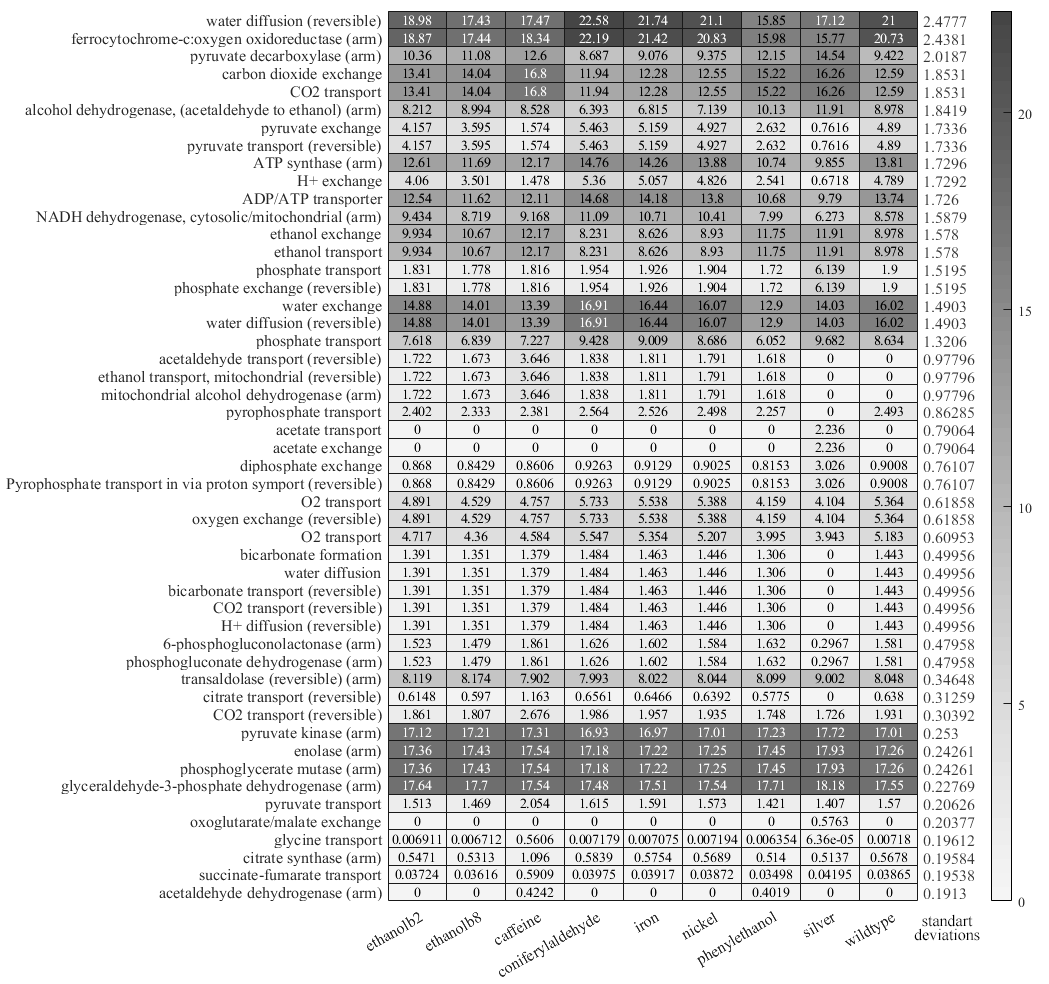
\includegraphics[width=1\columnwidth]{figures/fba_heatmap.png}
  \caption[Heatmap of the reaction fluxes where the standart deviation between models are the highest (top 50). Reversible means the intake of a substrate, arm means the flux of the reaction consists of isozyme reactions]{Heatmap of the reaction fluxes where the standart deviation between models are the highest (top 50). Reversible means the intake of a substrate, arm means the flux of the reaction consists of isozyme reactions.}
  \label{fig:fba_heatmap}
  \end{center}
\end{figure}

Overall the most divergent strain can be seen as silver resistant strain while the nickel strain has the closest values to the wildtype model as expected considering the integrated expression data. The highest deviation caused in the water diffusion from mitochondria to cytoplasm indicates that even at the same glucose feeding rates, phenylethanol resistant strain requires higher (89.5\%) water in the mitochondria. Followed with the ferrocytochrome-c:oxygen oxidoreductase, pyruvate decarboxylase reactions and different exchange reactions, the results conclude that the models of evolved strains follow different paths to produce biomass with the same environmental conditions provided.

As these different models belong the evolved strains, hierarchical relationship between models are drawn as dendrogram in Figure \ref{fig:fba_dendrogram}. Euclidean pairwise distance is calculated between flux balance analysis solution vectors for each model where the glucose uptake rate is constrained to 10 mmol/gDWh first and then clustered by the unweighted average distance (UPGMA) method to draw a tree. Cophenetic correlation coefficient is found as 0.9744 while theSpearman's rank correlation between the dissimilarities and the cophenetic distances is calculated as 0.9096, indicating a high-quality solution.

\begin{figure}[H]
  \begin{center}
  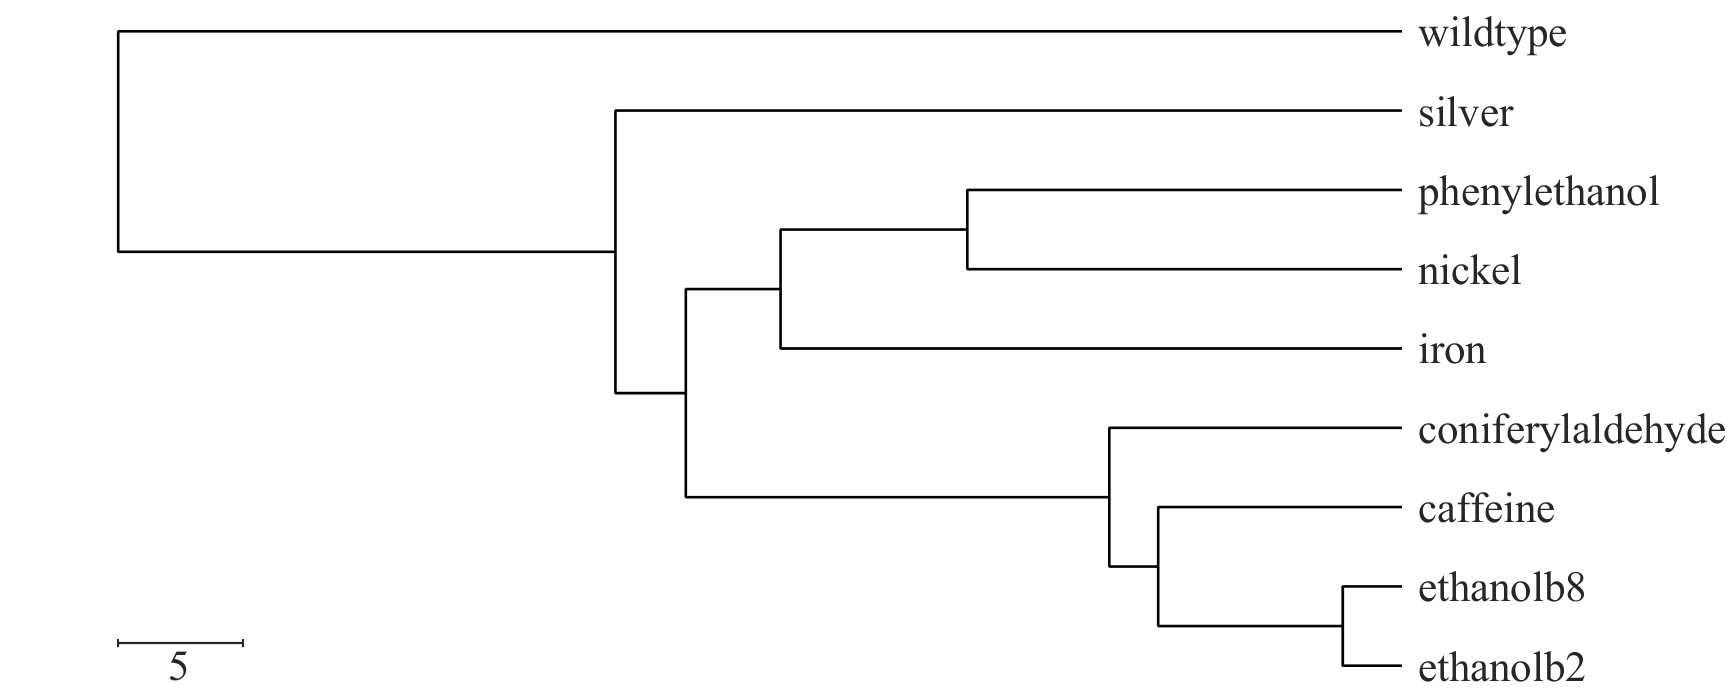
\includegraphics[width=1\columnwidth]{figures/fba_dendrogram.png}
  \caption[Hierarchical relationships between the strains drawn as a dendrogram plot. Euclidian distances are calcualted from the reaction fluxes (flux balance analysis) where the glucose uptake rate is constrained to 10 mmol/gDWh]{Hierarchical relationships between the strains drawn as a dendrogram plot. Euclidian distances are calcualted from the reaction fluxes (flux balance analysis) where the glucose uptake rate is constrained to 10 mmol/gDWh.}
  \label{fig:fba_dendrogram}
  \end{center}
\end{figure}

Despite the high correlation between the fold changes obtained from differential expression analysis and the flux balance analyses for particular enzymes, outliers must be investigated for the indirect regulation of enzymes. Three groups can be formed for these: Firstly, enzymes may show transcriptional regulation behaviors (TR) if their flux fold changes (between evolved and wildtype strain models) corralate with the differential gene expression results. Secondly, enzymes may show metabolic regulation behaviors (MR) if the flux change is observed even in the absences of the expressional changes. And lastly, enzymes may show post-transcriptional regulation behaviors (PR) if their expression levels change without showying any flux changes (Table \ref{table:regulation_table}). In the Figure \ref{fig:fba_regulation}, enzymes that have significant expressional fold changes (p $<$ 0.05) in all models are categorized for this purpose.

\vskip 1\baselineskip
\begin{table}[H]
\begin{center}
\caption[Enzymatic regulation decision table of expressional fold change (from differential analysis) and flux fold change (from flux balance analysis) comparison.]{Enzymatic regulation decision table of expressional fold change (from differential analysis) and flux fold change (from flux balance analysis) comparison.}
\vskip 0.5\baselineskip
\label{table:regulation_table}
\begin{tabular}{l|l|l|l|}
\cline{2-4}
\textbf{ExprFC \textbackslash FluxFC} & \textbf{Positive} & \textbf{Negative} & \textbf{No Change} \\ \hline
\multicolumn{1}{|l|}{\textbf{Positive}}  & Transcriptional & Metabolic       & Post-transcriptional \\ \hline
\multicolumn{1}{|l|}{\textbf{Negative}}  & Metabolic       & Transcriptional & Post-transcriptional \\ \hline
\multicolumn{1}{|l|}{\textbf{No Change}} & Metabolic       & Metabolic       &                      \\ \hline
\end{tabular}
\end{center}
\end{table}

Interestingly, most of the enzymes show post-transcriptional regulation behaviors indicating that even though the expression values are found significantly changed in the microarray analysis, their carried flux values did not differ in the \emph{in silico} simulations. Single simulation differences (such as FAS1, DFR1, CHO1 and ERG11 genes showing transcriptional regulation in all models except nickel model where they show metabolic regulation) must be investigated in order to understand the causal relationship.

\begin{figure}[H]
  \begin{center}
  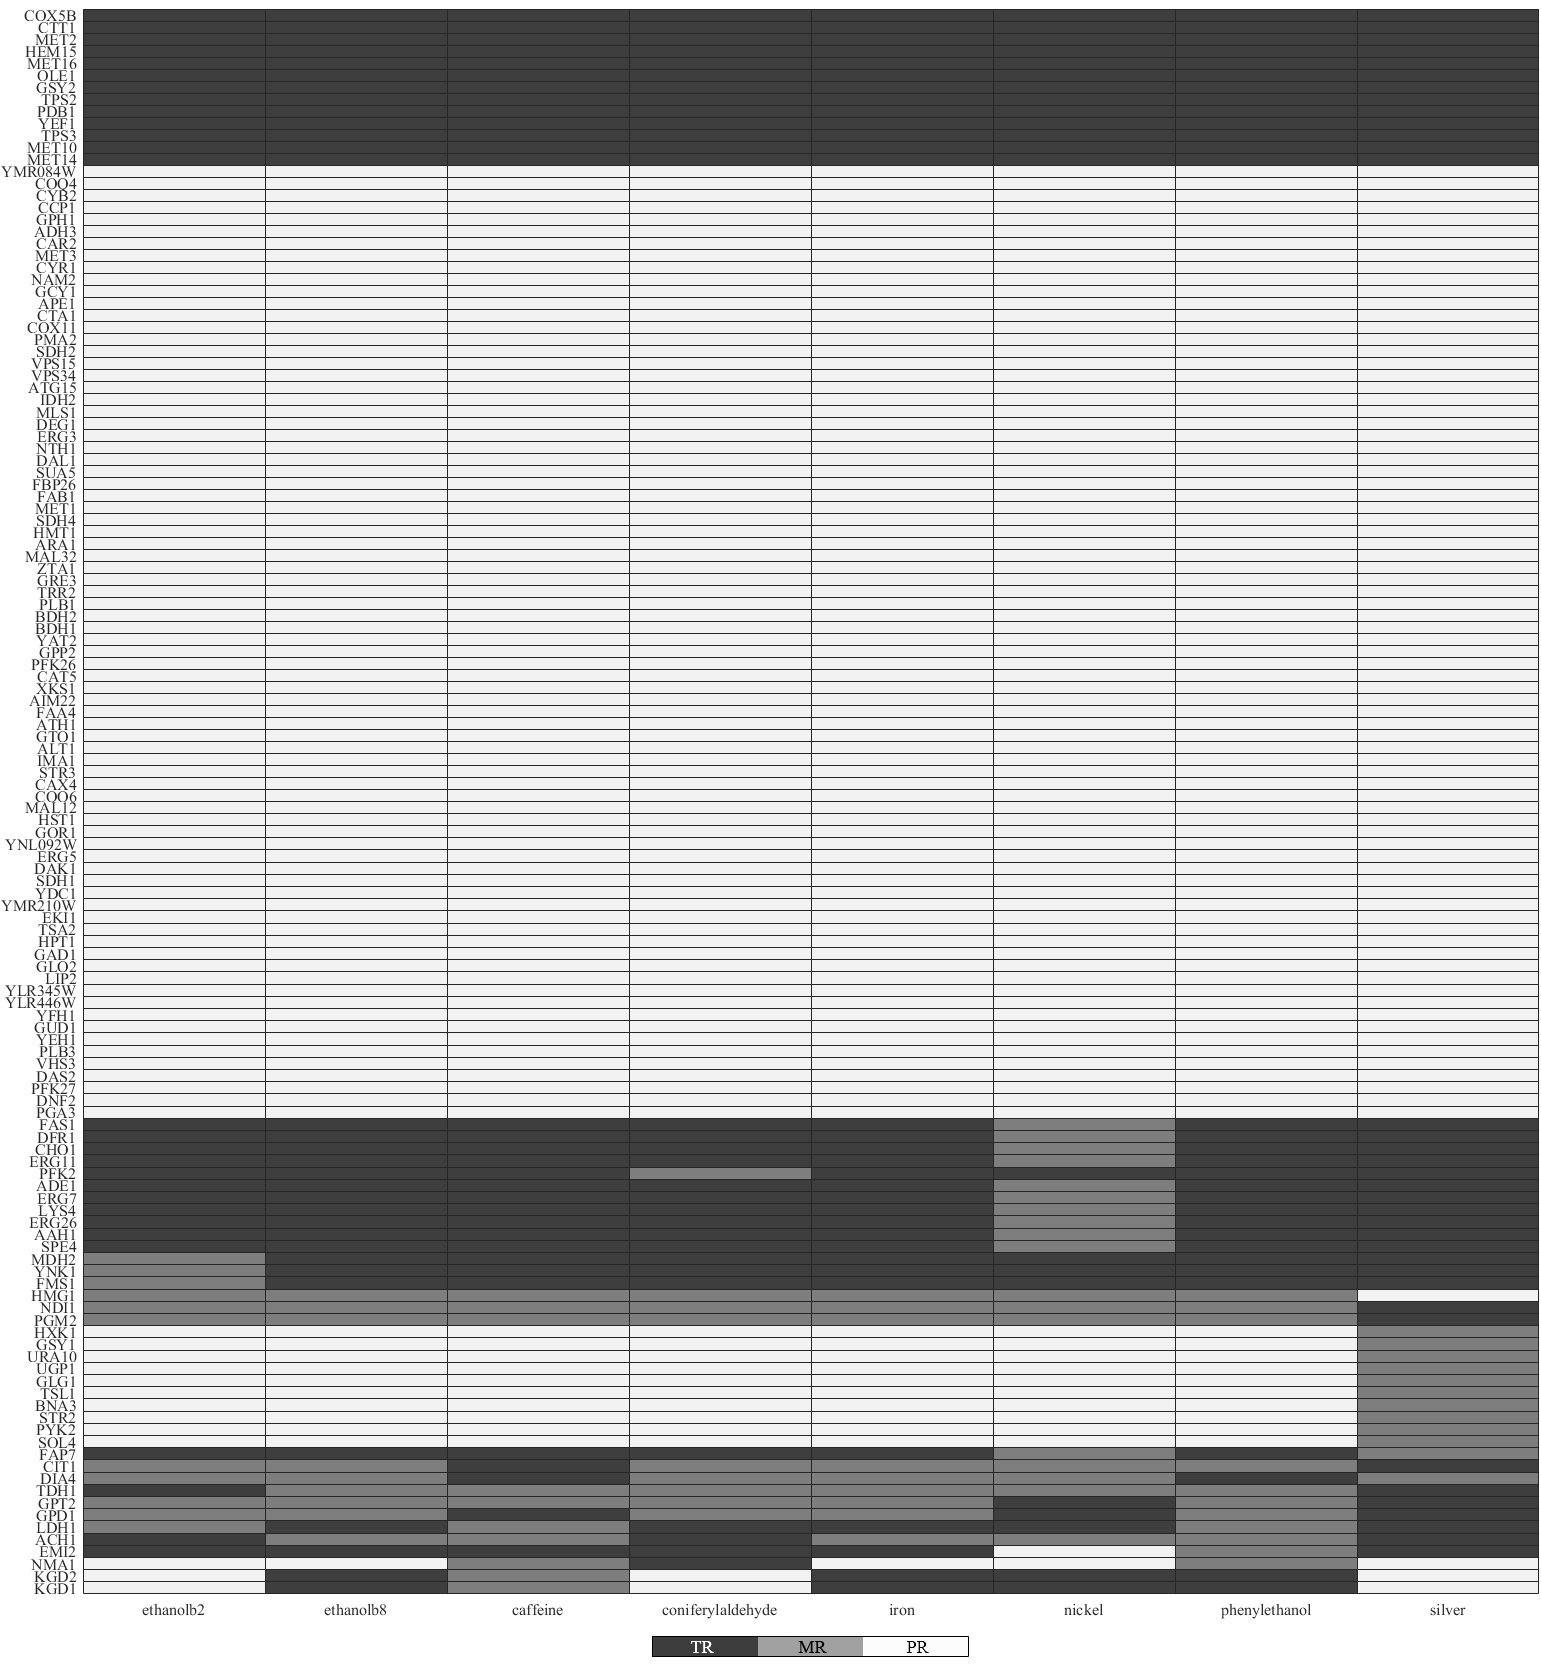
\includegraphics[width=1\columnwidth]{figures/fba_regulation.png}
  \caption[Categorization of enzymes for regulation points for transcriptional regulation (TR), metabolic regulation (MR), post-transcriptional regulation (PR)]{Categorization of enzymes for regulation points for transcriptional regulation (TR), metabolic regulation (MR), post-transcriptional regulation (PR).}
  \label{fig:fba_regulation}
  \end{center}
\end{figure}

\section{Flux Variability Analysis}
Flux ranges of each enzyme to find used enzymes and pathways on models are analyzed by the linear problem in the Flux Variability Analysis method where the objective functions to minimize and maximize all reactions iteratively with growth as the objective function kept at 90\%. Minimum and maximum available fluxes are collected in the iterative process for each reaction, and results are plotted in Figure \ref{fig:fva_enzymes}). Standart deviations on flux ranges for each reaction are also plotted to find most divergent targets. .

\begin{figure}[H]
  \begin{center}
  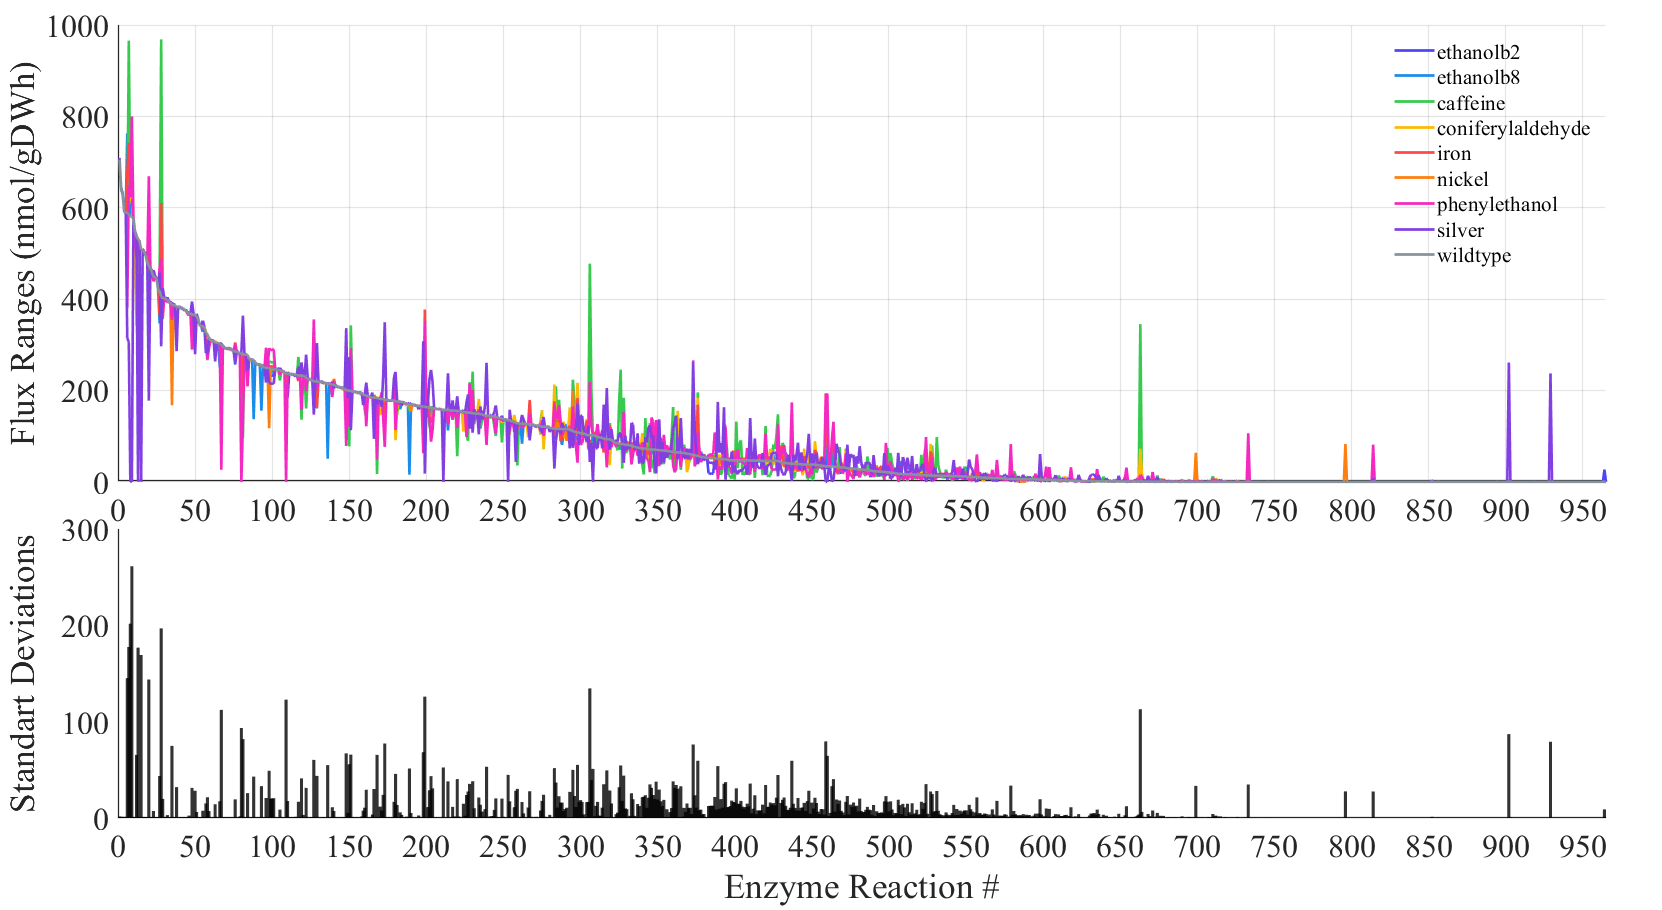
\includegraphics[width=1\columnwidth]{figures/fva_enzymes.png}
  \caption[Flux variability analysis results as flux ranges per enzyme usage reaction, sorted by the wild-type flux ranges]{Flux variability analysis results as flux ranges per enzyme usage reaction, sorted by the wild-type flux ranges.}
  \end{center}
  \label{fig:fva_enzymes}
  \end{figure}

As it can be seen in the Table \ref{table:fva_results} where the most divergent proteins (std $>$ 50) across all experiments are listed, paralog components of the glutathione system namely glutaredoxin-1 (GRX1) and glutaredoxin-2 (GRX2) shows the highest divergence across strains, followed by the glyceraldehyde-3-phosphate dehydrogenase (GAPDH) isozymes, triose-phosphate dehydrogenase 2 and 3 (TDH3 and TDH2).

\begin{table}[H]
\footnotesize
\caption[The most (std $>$ 55 nmol/gDWh) divergent proteins across all experiments and their flux variabilities as ranges (max - min flux) in nmol/gDWh]{The most (std $>$ 55 nmol/gDWh) divergent proteins across all experiments and their flux variabilities as ranges (max - min flux) in nmol/gDWh.}
\vspace{0.3cm}
\begin{center}
  \setlength{\tabcolsep}{4pt}
  \resizebox{\textwidth}{!}{
  \begin{tabular}{|c|c|c|c|c|c|c|c|c|c|c|}
    \hline
\textbf{Enzyme} & \textbf{b2-ethanol} & \textbf{b8-ethanol} & \textbf{caffeine} & \textbf{\begin{tabular}[c]{@{}l@{}}coniferyl \\ aldehyde\end{tabular}} & \textbf{iron} & \textbf{nickel} & \textbf{\begin{tabular}[c]{@{}l@{}}phenyl \\ ethanol\end{tabular}} & \textbf{silver} & \textbf{reference} & \textbf{std} \\ \hline

%
GRX1            & 580.52             & 798.71             & 796.91            & 799.92                     & 799.02        & 580.52          & 799.86                 & 0               & 580.52            & 261.34       \\ \hline
GRX2            & 580.52             & 580.52             & 622.01            & 624.36                     & 623.65        & 580.52          & 622.86                 & 0.08            & 580.52            & 201.73       \\ \hline
TDH3            & 561.29             & 609.88             & 968.54            & 403.74                     & 610.11        & 404.14          & 488.51                 & 296.71          & 403.66            & 196.83       \\ \hline
TDH2            & 702.15             & 760.74             & 965.83            & 607.13                     & 742.34        & 584.58          & 649.07                 & 305.09          & 586.70            & 177.49       \\ \hline
HYR1            & 530.62             & 530.44             & 529.25            & 531.24                     & 530.65        & 531.78          & 529.97                 & 0               & 531.14            & 176.88       \\ \hline
GPX1            & 507.66             & 507.49             & 506.35            & 508.26                     & 507.69        & 508.74          & 507.04                 & 0               & 508.16            & 169.23       \\ \hline
TDH1            & 704.05             & 762.80             & 542.42            & 606.64                     & 672.41        & 586.16          & 381.54                 & 315.49          & 588.29            & 145.14       \\ \hline
OLI1            & 498.12             & 447.32             & 256.85            & 462.14                     & 503.37        & 480.46          & 668.93                 & 177.89          & 471.85            & 143.72       \\ \hline
TRX2            & 83.56              & 76.81              & 477.59            & 85.43                      & 91.79         & 101.72          & 218.84                 & 43.53           & 102.17            & 134.54       \\ \hline
SOL4            & 239.80             & 324.14             & 363.99            & 365.53                     & 377.35        & 156.46          & 351.92                 & 18.15           & 164.11            & 126.02       \\ \hline
ERG10           & 237.06             & 236.98             & 0.01              & 0.02                       & 0.02          & 214.75          & 0.01                   & 238.31          & 237.27            & 122.94       \\ \hline
CYC7            & 3.07               & 6.00               & 345.15            & 72.74                      & 10.38         & 1.24            & 15.25                  & 0.07            & 0.55              & 112.84       \\ \hline
AYR1            & 274.31             & 301.45             & 301.68            & 63.66                      & 301.41        & 301.16          & 26.45                  & 302.96          & 301.69            & 112.20       \\ \hline
PGA3            & 280.31             & 280.22             & 279.59            & 280.28                     & 280.33        & 280.16          & 0                      & 281.75          & 280.59            & 93.47        \\ \hline
SNO3            & 0                  & 0                  & 0                 & 0                          & 0             & 0               & 0                      & 261.32          & 0                 & 87.11        \\ \hline
DAS2            & 259.51             & 224.29             & 96.71             & 211.09                     & 191.35        & 276.99          & 126.60                 & 363.82          & 279.13            & 81.82        \\ \hline
HXK1            & 82.23              & 146.33             & 188.50            & 189.24                     & 193.89        & 33.59           & 186.56                 & 0.01            & 34.44             & 79.54        \\ \hline
SNO2            & 0                  & 0                  & 0                 & 0                          & 0             & 0               & 0                      & 237.53          & 0                 & 79.18        \\ \hline
URA6            & 153.11             & 148.21             & 113.37            & 133.15                     & 123.92        & 175.63          & 76.48                  & 349.32          & 179.93            & 77.32        \\ \hline
YDC1            & 265.82             & 137.27             & 265.96            & 265.85                     & 265.50        & 265.13          & 265.98                 & 261.85          & 58.55             & 76.34        \\ \hline
YOR283W         & 385.25             & 284.27             & 374.59            & 386.44                     & 383.88        & 167.70          & 354.85                 & 391.22          & 387.67            & 74.91        \\ \hline
SOL3            & 173.27             & 160.34             & 102.97            & 127.45                     & 116.01        & 161.25          & 62.84                  & 307.74          & 165.03            & 68.26        \\ \hline
CDC8            & 180.45             & 172.85             & 222.25            & 182.36                     & 168.37        & 198.14          & 78.50                  & 336.56          & 201.04            & 67.03        \\ \hline
ALG13           & 222.59             & 233.87             & 342.51            & 266.53                     & 268.81        & 198.78          & 292.49                 & 113.05          & 199.23            & 65.73        \\ \hline
GPX2            & 537.40             & 537.23             & 536.02            & 341.26                     & 537.43        & 538.58          & 488.86                 & 540.21          & 537.93            & 65.52        \\ \hline
PDC5            & 157.75             & 161.29             & 17.12             & 185.99                     & 76.60         & 181.67          & 48.37                  & 169.86          & 183.92            & 65.47        \\ \hline
GLK1            & 27.76              & 50.03              & 133.67            & 135.09                     & 92.54         & 33.06           & 193.48                 & 0               & 34.35             & 64.44        \\ \hline
GPP2            & 204.17             & 215.88             & 261.44            & 299.76                     & 230.49        & 212.94          & 355.61                 & 147.19          & 219.99            & 60.29        \\ \hline
ALD4            & 44.53              & 37.53              & 140.64            & 138.00                     & 78.24         & 40.30           & 174.06                 & 1.32            & 39.86             & 59.43        \\ \hline
PYK2            & 91.09              & 88.38              & 195.97            & 183.93                     & 169.19        & 55.15           & 108.01                 & 38.43           & 56.16             & 59.39        \\ \hline
ALG14           & 179.10             & 169.99             & 77.84             & 142.43                     & 140.31        & 198.78          & 120.83                 & 273.04          & 199.23            & 55.73        \\ \hline
MHT1            & 107.29             & 91.30              & 170.34            & 216.78                     & 183.08        & 108.03          & 41.78                  & 171.04          & 108.32            & 55.14        \\ \hline

\end{tabular}}
\label{table:fva_results}
\end{center}
\end{table}


Pathway-wise investigation is carried out from the flux variability analysis results. First, the reactions that have subsystem annotations are collected for each seperately. It must be noted that some reactions can exist in multiple subsystems, for example, phosphoenolpyruvate carboxykinase reaction exists in all gluconeogenesis, glycolysis, citrate cycle (TCA cycle), pyruvate metabolism, biosynthesis of secondary metabolites, biosynthesis of antibiotics, and carbon metabolism subsystems. Secondly, the mean flux values for each subsystem for all models in flux variability analysis are collected. These flux values for the most common subsystems are plotted as stacked bars in Figure \ref{fig:fva_subsystem_spans} to distinguish subsystem activity for each model after the normalization arised from the assumption of the total flux value for each model should be equal in order to allow comparison.

\begin{figure}[H]
  \begin{center}
  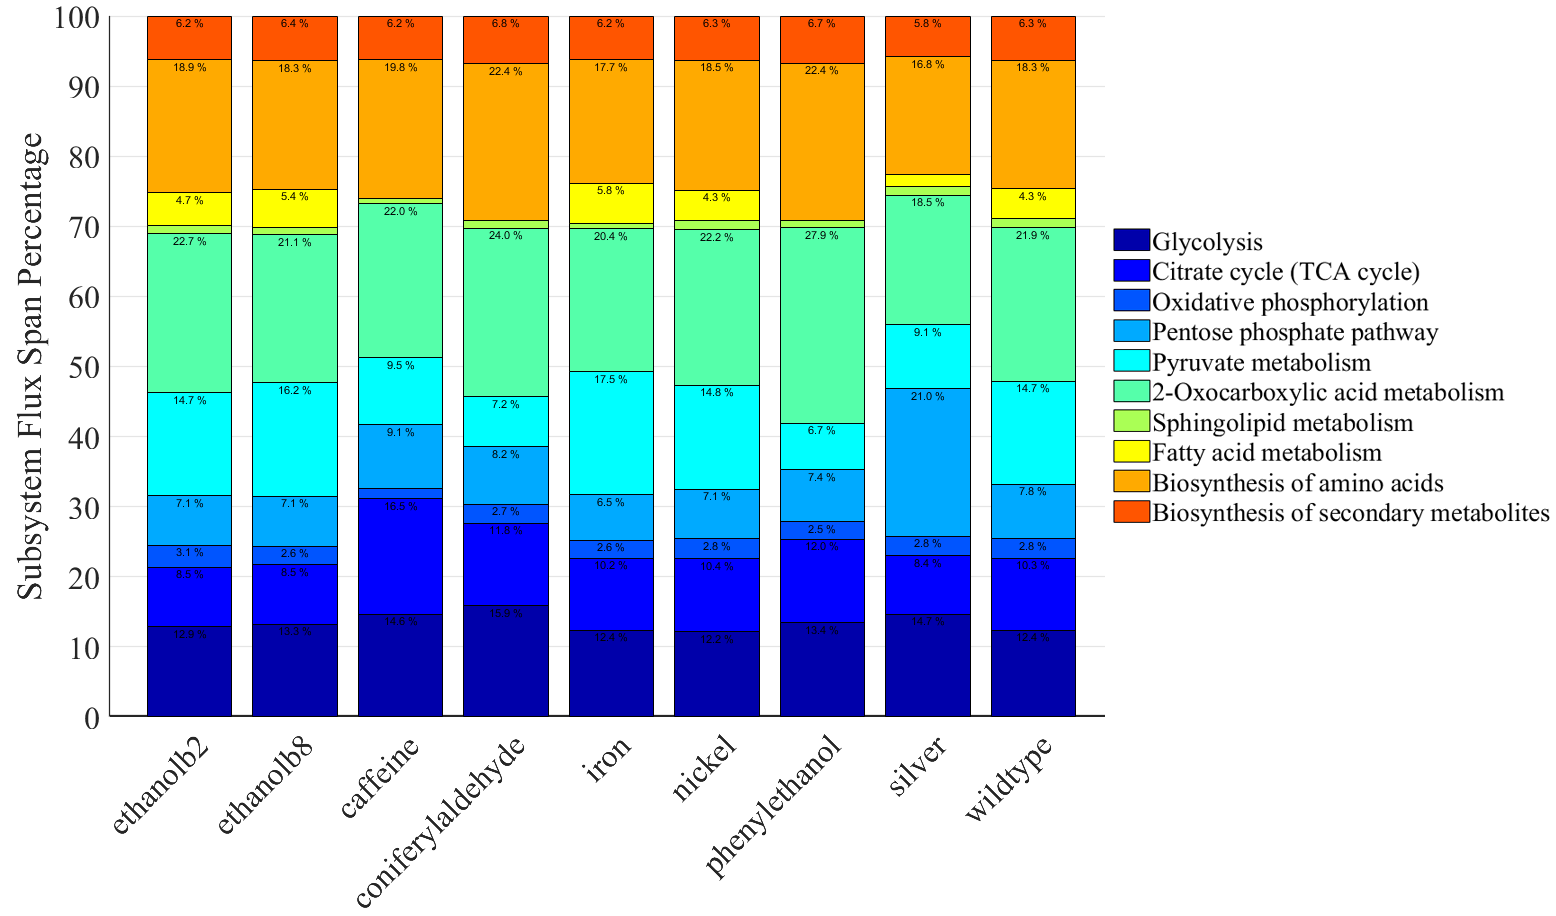
\includegraphics[width=1\columnwidth]{figures/fva_subsystem_spans.png}
  \caption[Mean carried fluxes through the ubsystems are shown as stacked bars for strain-wise comparison. Sum of fluxes are normalized to a hundred percent to be able to distinguish flux distribution]{Mean carried fluxes through the ubsystems are shown as stacked bars for strain-wise comparison. Sum of fluxes are normalized to a hundred percent to be able to distinguish flux distribution.}
  \label{fig:fva_subsystem_spans}
  \end{center}
\end{figure}

Despite the similarities in the flux values some of the subsystems, interesting results are observed. The most distinguished models are observed as caffeine, coniferylaldehyde and phenylethanol strains as they do not carry fluxes through fatty acid metabolism reactions. Instead, the caffeine model shows higher activity in the TCA cycle reactions, compared to coniferylaldehyde and phenylethanol strains where the activity increases in the 2-oxocarboxylic acid metabolism.

\section{Survivability Analysis: Knock-out Simulations}
To calculate the essentiality of the reactions and the proteins on the growth, \emph{in-silico} single deletion analyses are done on all the reactions for each model. Growth rate ratios between deletion applied models and the prior models are collected as percentages for each strain. The reactions that have the same value for each experiment are discarded from the results considering they do not differ after evolution. To be able to catch the most important proteins, only the reactions with the minimum of \%95 growth rate decreases are reported here. The impacts of the deleted reactions are seperately shown as heatmaps in Figure \ref{fig:deletion_survivability_rxns} for metabolic reactions and in Figure \ref{fig:deletion_survivability_prots} proteins.

\begin{figure}[H]
  \begin{center}
  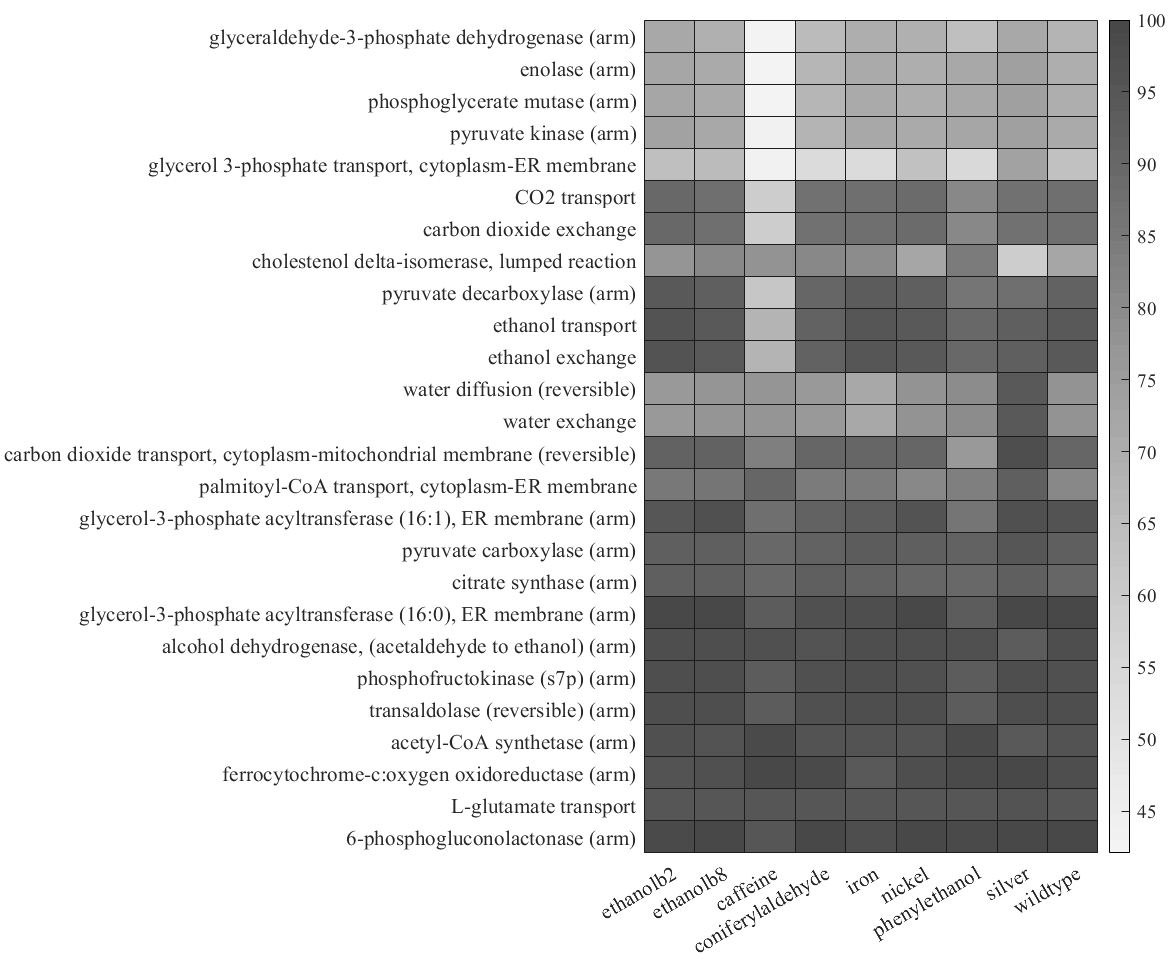
\includegraphics[width=1\columnwidth]{figures/deletion_survivability_rxns.png}
  \caption[Heatmaps of the growth rate ratios between deletion strains for each experiment. The knocked-out reactions that cause a decrease higher than \%95 are reported.]{Heatmaps of the growth rate ratios between deletion strains for each experiment. The knocked-out reactions that cause a decrease higher than \%95 are reported.}
  \label{fig:deletion_survivability_rxns}
  \end{center}
\end{figure}

\begin{figure}[H]
  \begin{center}
  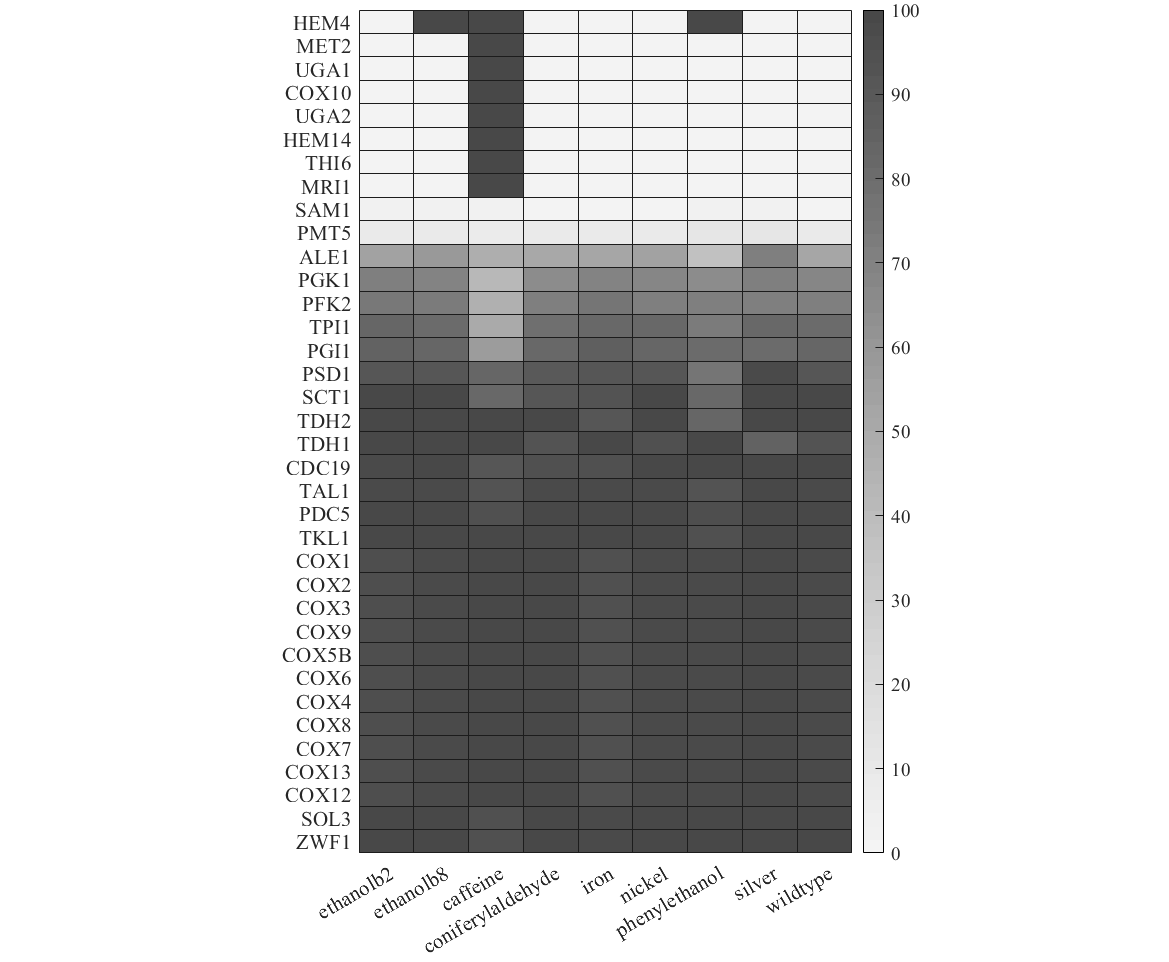
\includegraphics[width=1\columnwidth]{figures/deletion_survivability_prots.png}
  \caption[Heatmaps of the growth rate ratios between deletion strains for each experiment. The knocked-out proteins that cause a decrease higher than \%95 are reported.]{Heatmaps of the growth rate ratios between deletion strains for each experiment. The knocked-out proteins that cause a decrease higher than \%95 are reported.}
  \label{fig:deletion_survivability_prots}
  \end{center}
\end{figure}

Although all the models were able to grow in any single deletion on the reactions (with the minimum 45\% lower growth rate from the non-deletion models), 2 enzymes (SAM1 and PMT5) are found essential for all models. Interestingly, MET2, UGA1, COX10, UGA2, HEMI4, THI6 and MRI1 enzymes were essential for all models except the caffeine-resistant model. On the other hand, the deletion of the PGK1, PFK2, TPI1 and PFI1 enzymes decreases the caffeine-resistant model's growth ability higher than other models.

\section{Minimization of Metabolic Adjustment}

Minimization of metabolic adjustment (MOMA) analysis is applied to evolved models to find the closest points to wild-type model simulations (in terms of the Euclidean distances). Analysis is done with the objective of maximization of the growth rate and no constraints applied to the models except for the total protein amount availability. Results are collected for the metabolic reactions and the proteins (as enzyme-draw reactions) seperately. The sum of the distances from the wildtype simulations is used as a ranking system to find most distant reactions and proteins. Individual fluxes through reactions can be seen in Figure \ref{fig:moma_cumdist}.


 The most distant reactions in the evolved models from the wild type model found as palmitoyl-CoA hydrolase, followed by the long chain fatty acid CoA ligase, deoxyuridine kinase, methylglyoxal synthase, 5' nucleotidases, glutathione metabolism reactions. On the other hand, the enzymes TDH1 (glyceraldehyde-3-phosphate dehydrogenase isozyme 1), OLI1 (F0 ATP synthase subunit c), GPT2 (glycerol-3-phosphate/dihydroxyacetone phosphate sn-1 acyltransferase), RIB7 (Diamino-hydroxy-phoshoribosyl-amino-pyrimidine deaminase), SCT1 (glycerol 3-phosphate/dihydroxyacetone phosphate sn-1 acyltransferase) and COB (cytochrome b) were the top distant enzymes in terms of enzyme-draw reaction fluxes.

\begin{figure}[H]
  \begin{center}
  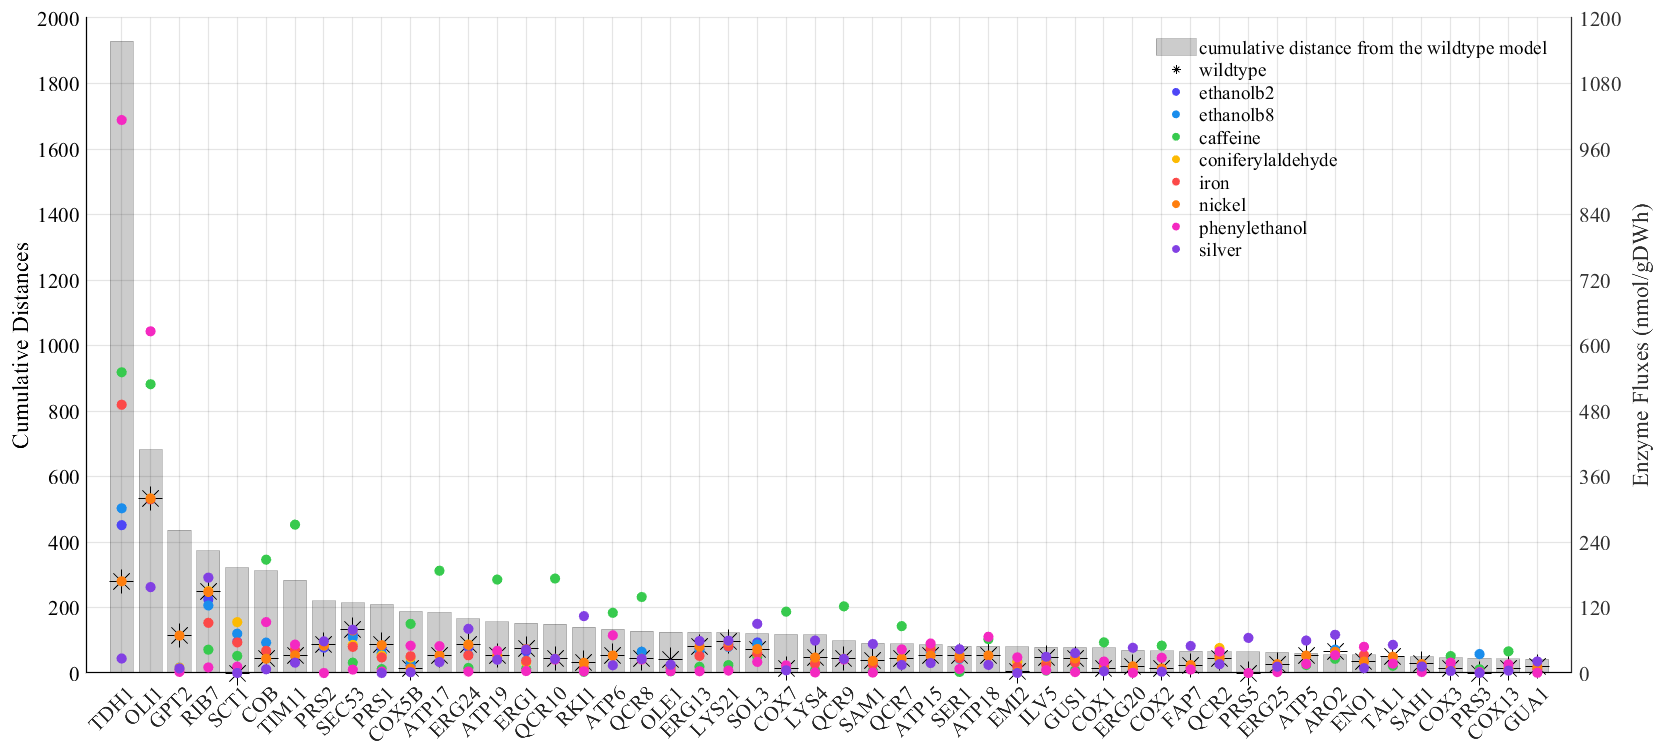
\includegraphics[width=1\columnwidth]{figures/moma_cumdist.png}
  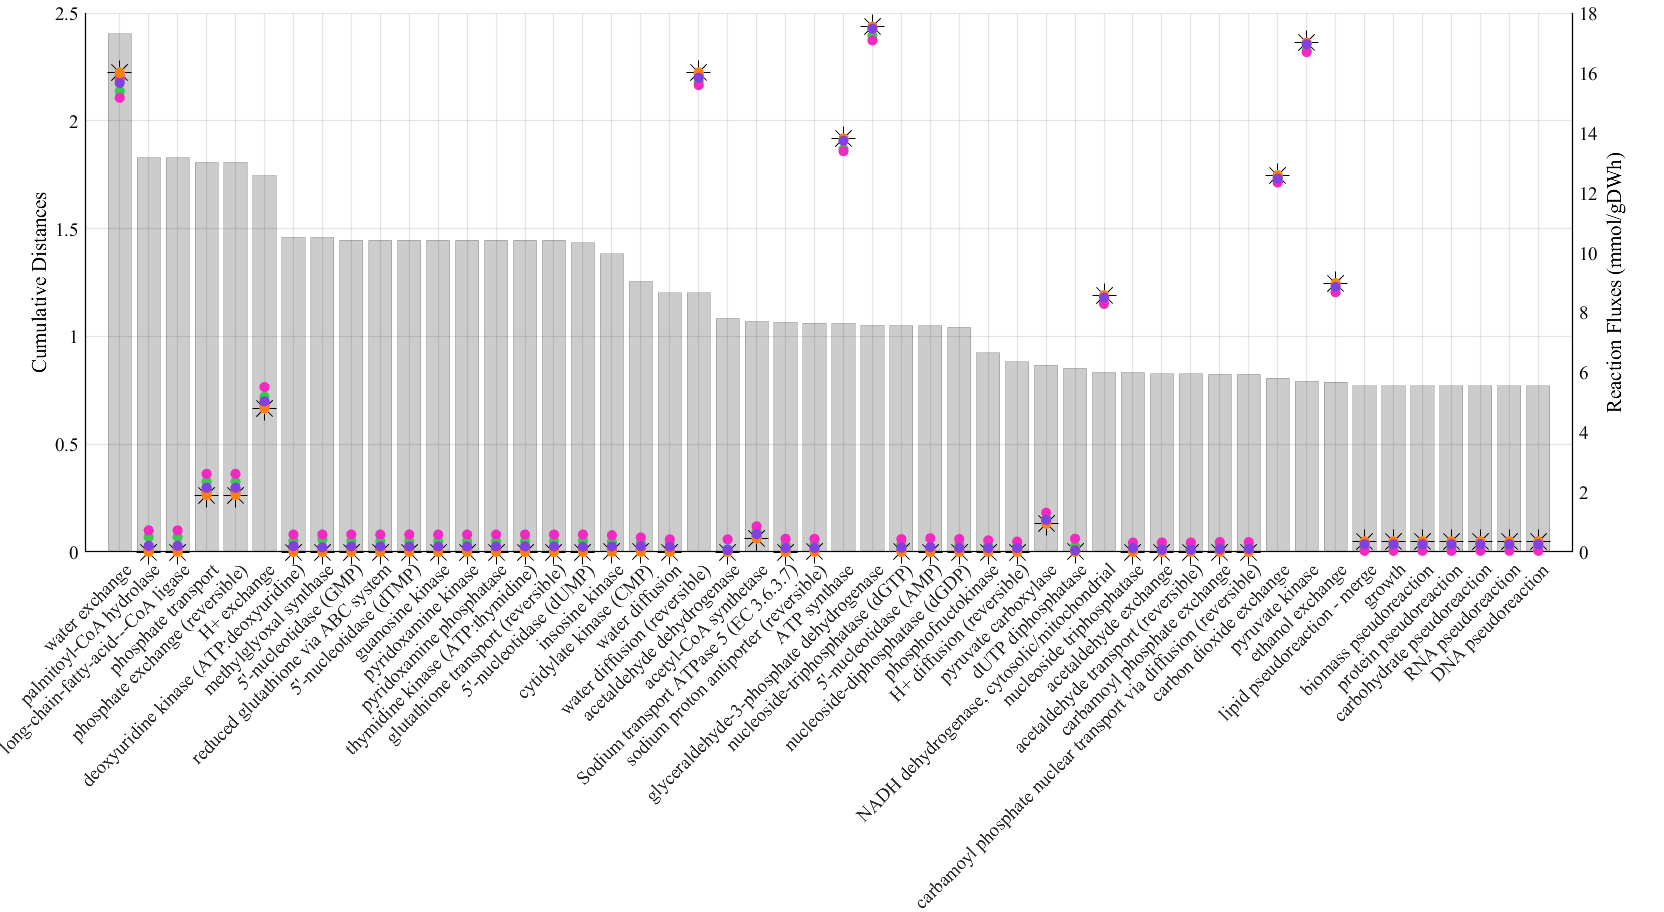
\includegraphics[width=1\columnwidth]{figures/moma_cumdist_rxns.png}
  \caption[Enzymes that have MOMA flux values the most distant from the wild-type flux values in nmol/gDWh]{Enzymes that have MOMA flux values the most distant from the wild-type flux values in nmol/gDWh.}
  \label{fig:moma_cumdist}
  \end{center}
\end{figure}

\section{Sampling Results}

The random solutions for each metabolic models are obtained by maximizing  for a random set of three reactions with random weights. Total of 10,000 solutions for each model are generated after the boundaries on growth rate as an objective function is set to minimum of 90\% and maximum of 100\% growth rate of the flux balance analysis results. The solution spaces for these reactions are plotted as histogram plots where the bin counts, N, are normalized so that the sum(N) is 1 for each analysis.

The most divergent reactions excluding diffusion, transport and exchange reactions from FBA results are plotted in Figure \ref{fig:sampling_fba_top12}, the most divergent enzymes from FVA results are plotted in Figure \ref{fig:sampling_fva_top12}, followed by the MOMA hits in Figure \ref{fig:sampling_moma_top12}.

\begin{figure}[H]
  \begin{center}
  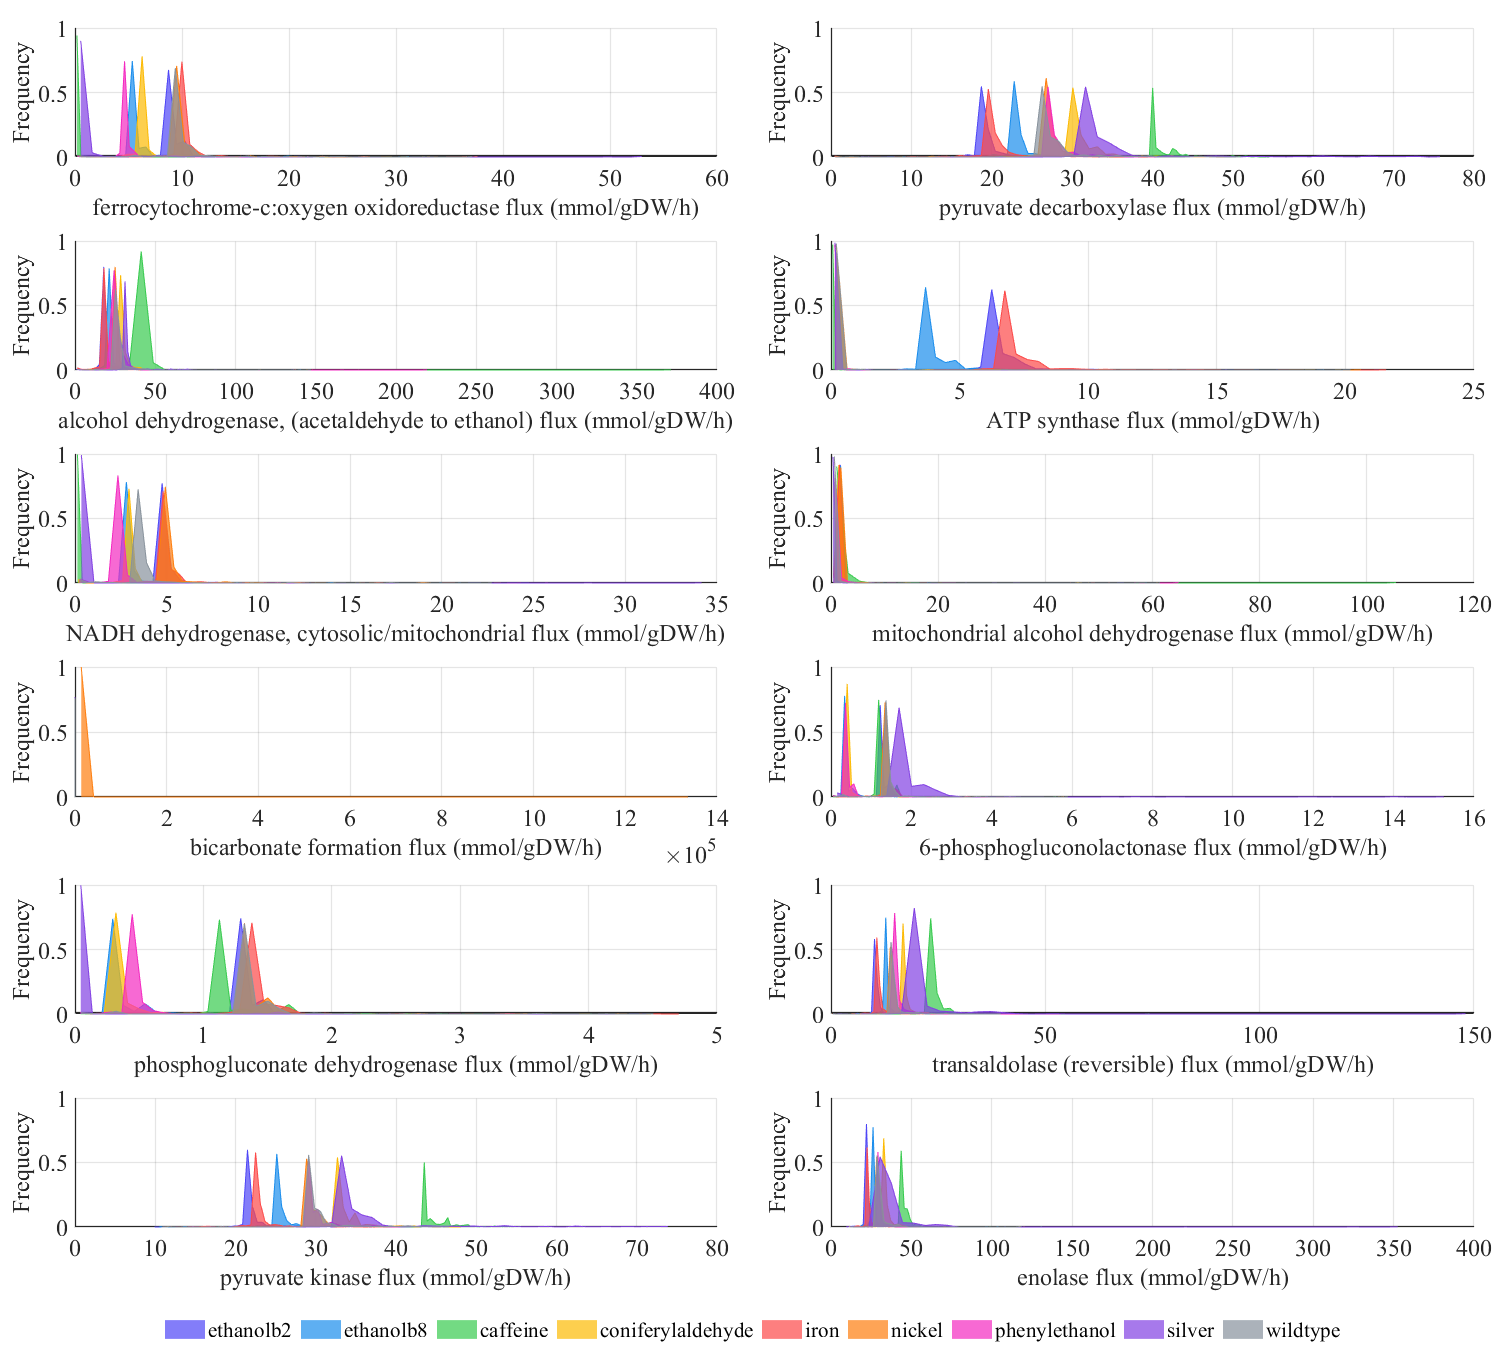
\includegraphics[width=1\columnwidth]{figures/sampling_fba_top12.png}
  \caption[Flux distributions of the reactions that diverge the most in flux balance analysis, obtained from the random sampling of solution spaces for each model shown as histogram plots]{Flux distributions of the reactions that diverge the most in flux balance analysis, obtained from the random sampling of solution spaces for each model shown as histogram plots.}
  \label{fig:sampling_fba_top12}
  \end{center}
\end{figure}

Ferrocytochrome-c:oxygen oxidoreductase reaction shows a great divergence across all models despite having the 0 flux on the caffeine resistant model. This 0 flux on the caffeine model explains the higher fluxes through alcohol dehydrogenase reaction, meaning thet the oxidative phosphorylation rates are lower in the cafferine resistant model compared to ethanol producing pathways. Pyruvate decarboxylase reaction shows almost the pattern with the pyruvate kinase reaction indicating a chain reaction. Remember that the although the models are fed with the same amount of carbon sources, small differences in their reaction fluxes comes from the adaptive evolution expression analyses. That reminded, the small flux values on the 6-phosphogluconolactonase reaction biologically may not mean a big difference, however the different behavior of the silver resistant model (having a wider range over other models) could mean the availability of the althernative pathways for the same biological objective.


\begin{figure}[H]
  \begin{center}
  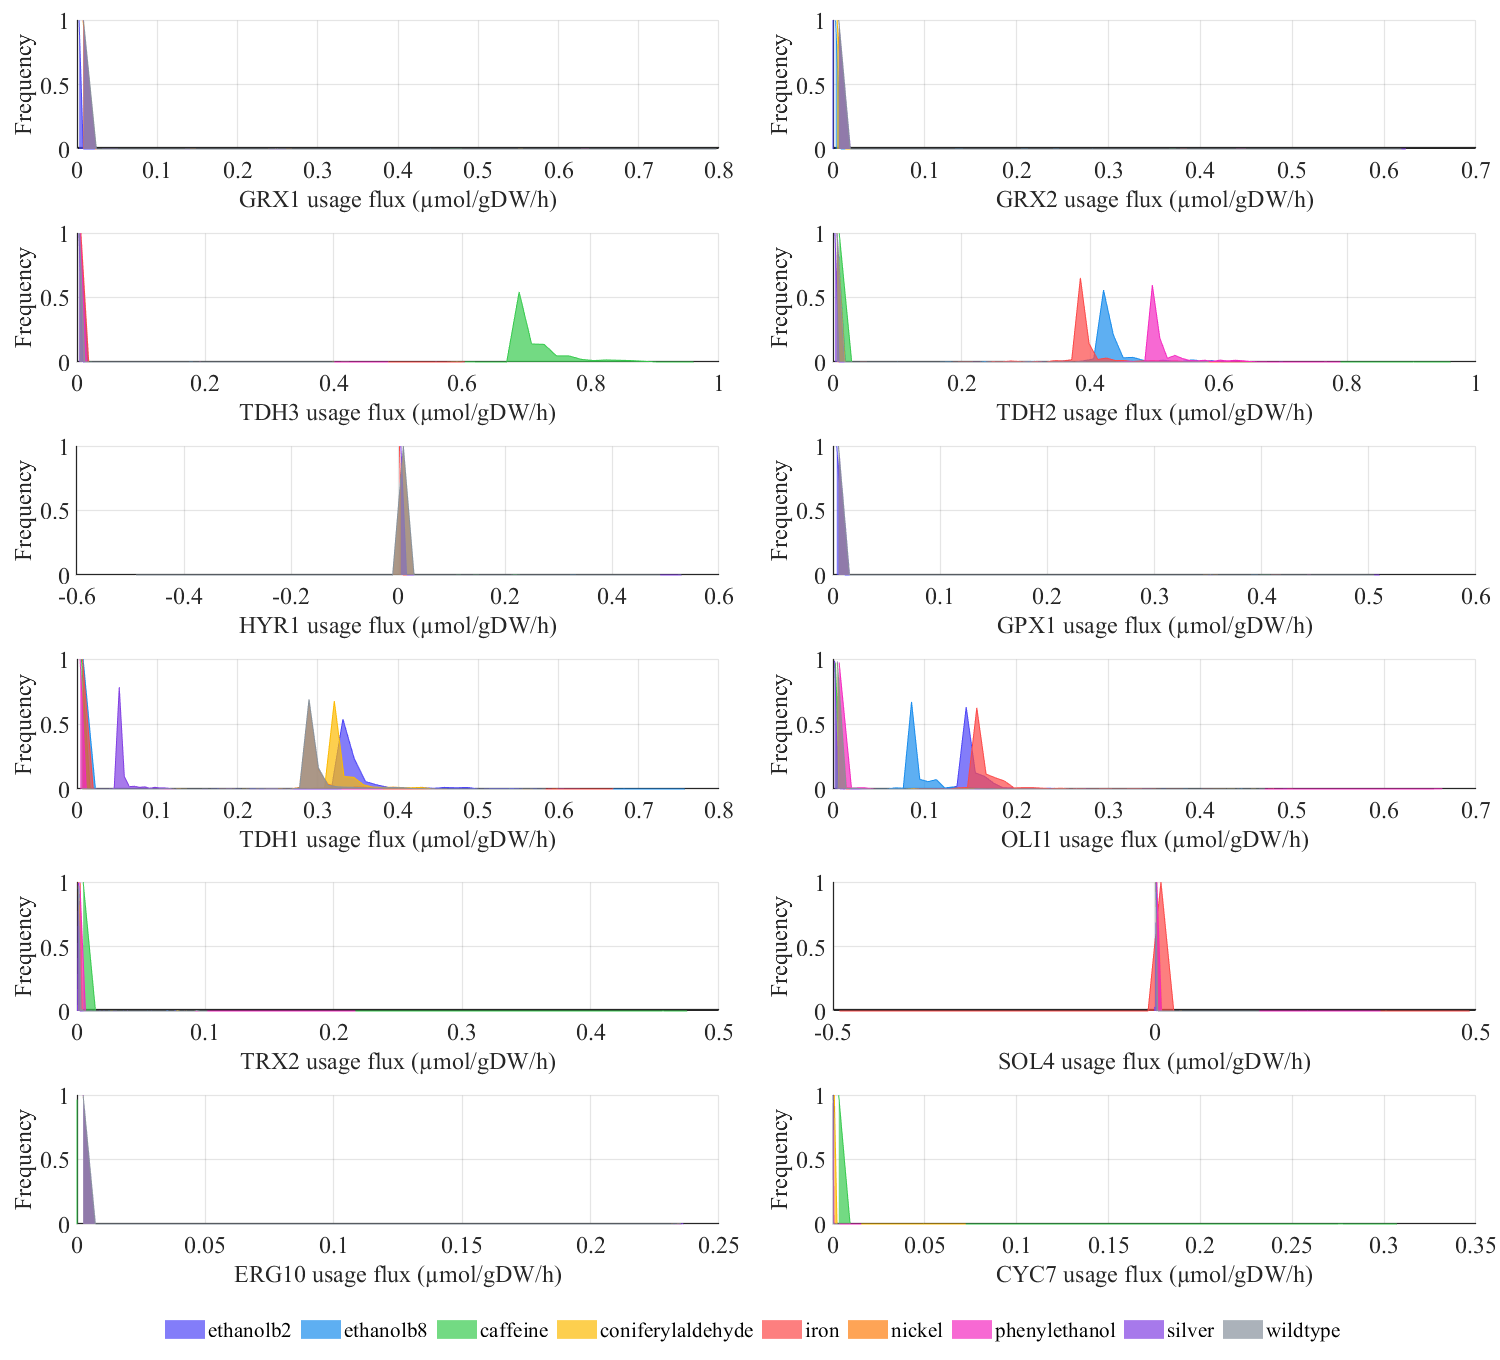
\includegraphics[width=1\columnwidth]{figures/sampling_fva_top12.png}
  \caption[Flux distributions of the reactions that diverge the most in flux variability analysis, obtained from the random sampling of solution spaces for each model shown as histogram plots]{Flux distributions of the reactions that diverge the most in flux variability analysis, obtained from the random sampling of solution spaces for each model shown as histogram plots.}
  \label{fig:sampling_fva_top12}
  \end{center}
\end{figure}

Enzyme fluxes are numerically hard to distinguish in histogram plots because of the lower magnitude of the enzyme kinetics. The main target enzymes from the flux variability analysis are found as the glutaredoxin paralogs (GRX1 and GRX2) mostly did not show a very different behaviors on the sampled solution spaces. Glyceraldehyde-3-phosphate dehydrogenase isozymes (TDH1, TDH2 and TDH3) on the other hand show the different preferences between models.

In order to investigate enzyme relationships, correlation coefficients for each enzyme is calculated from the solution spaces for all models. Considering only the correlation values higher than R $>$ 0.5, GRX enzymes are found the be positively correlated with the phospholipid hydroperoxide glutathione peroxidase (GPX) enzymes (Figure \ref{fig:sampling_correlation_grx}).

\begin{figure}[H]
  \begin{center}
  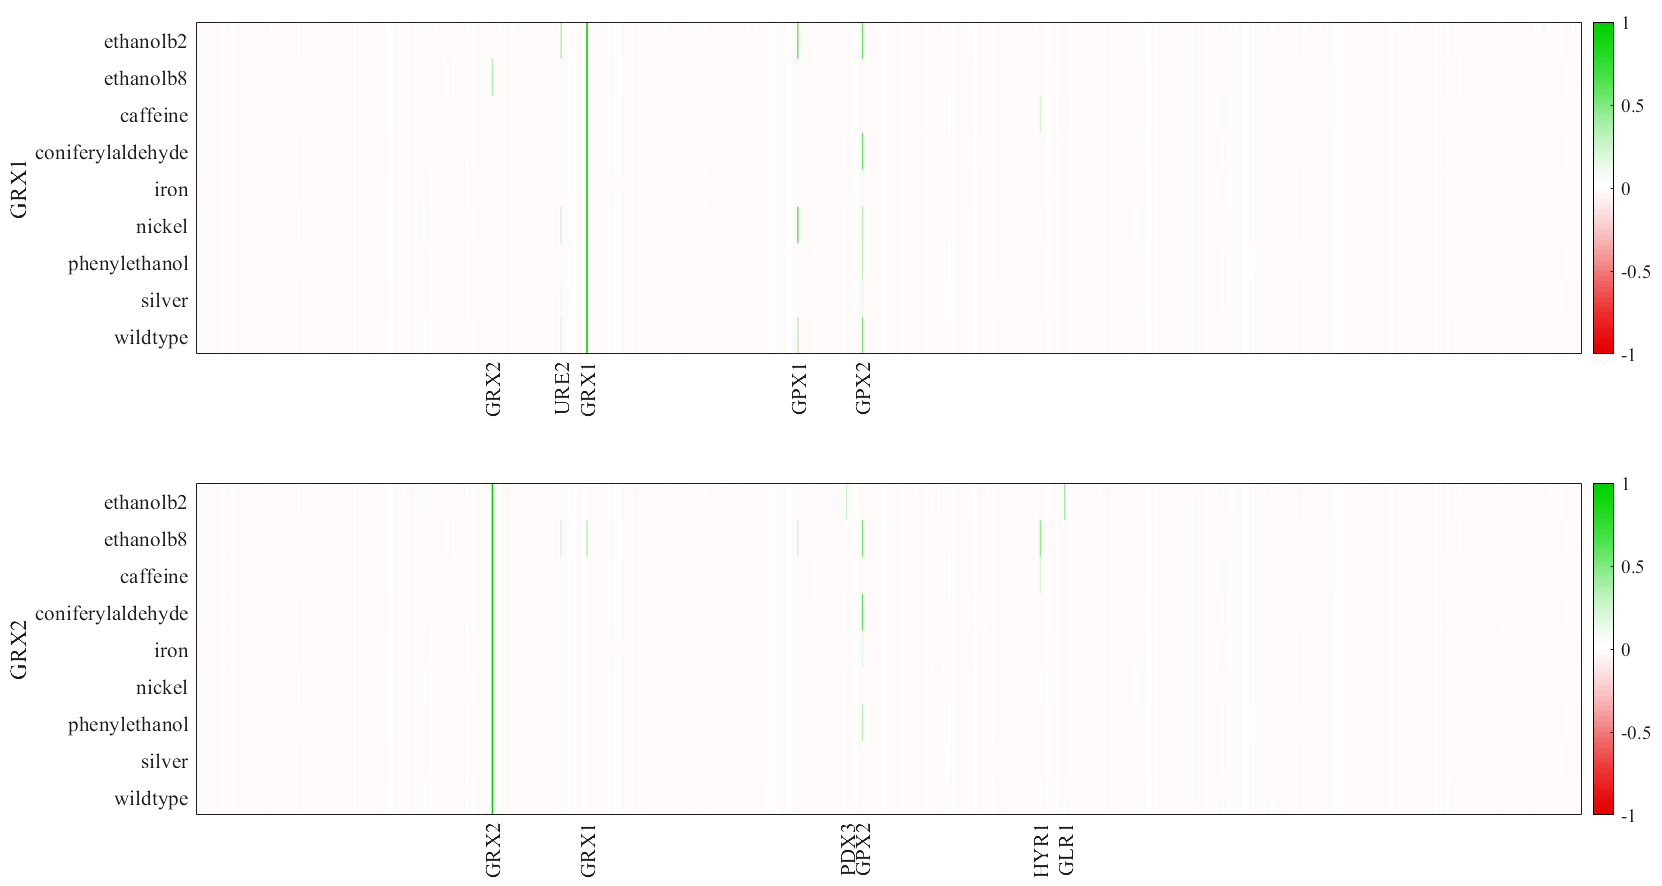
\includegraphics[width=1\columnwidth]{figures/sampling_correlation_grx.png}
  \caption[Correlations of GRX1 (top) and GRX2 (bottom) enzymes to other enzymes calculated from the random sampling of solution spaces. Only the name of enzymes with the correlation value c$>$0.8 are shown in the y-axes]{Correlations of GRX1 (top) and GRX2 (bottom) enzymes to other enzymes calculated from the random sampling of solution spaces. Only the name of enzymes with the correlation value c$>$0.3 are shown in the y-axes}
  \label{fig:sampling_correlation_grx}
  \end{center}
\end{figure}

TDH3 enzyme shows positive correlation only in the caffeine resistant model to 4 enzymes: An enzyme responsible for the regulation of telomerase (CDC13), minor isoform of pyruvate decarboxylase (PDC5), subunit of phosphofructokinase (PFK2), and to a protein of unknown function (EMI2). TDH1 and TDH3 enzymes on the other hand show both positive and negative correlations to multiple enzymes (Figure \ref{fig:sampling_correlation_tdh}).

\begin{figure}[H]
  \begin{center}
  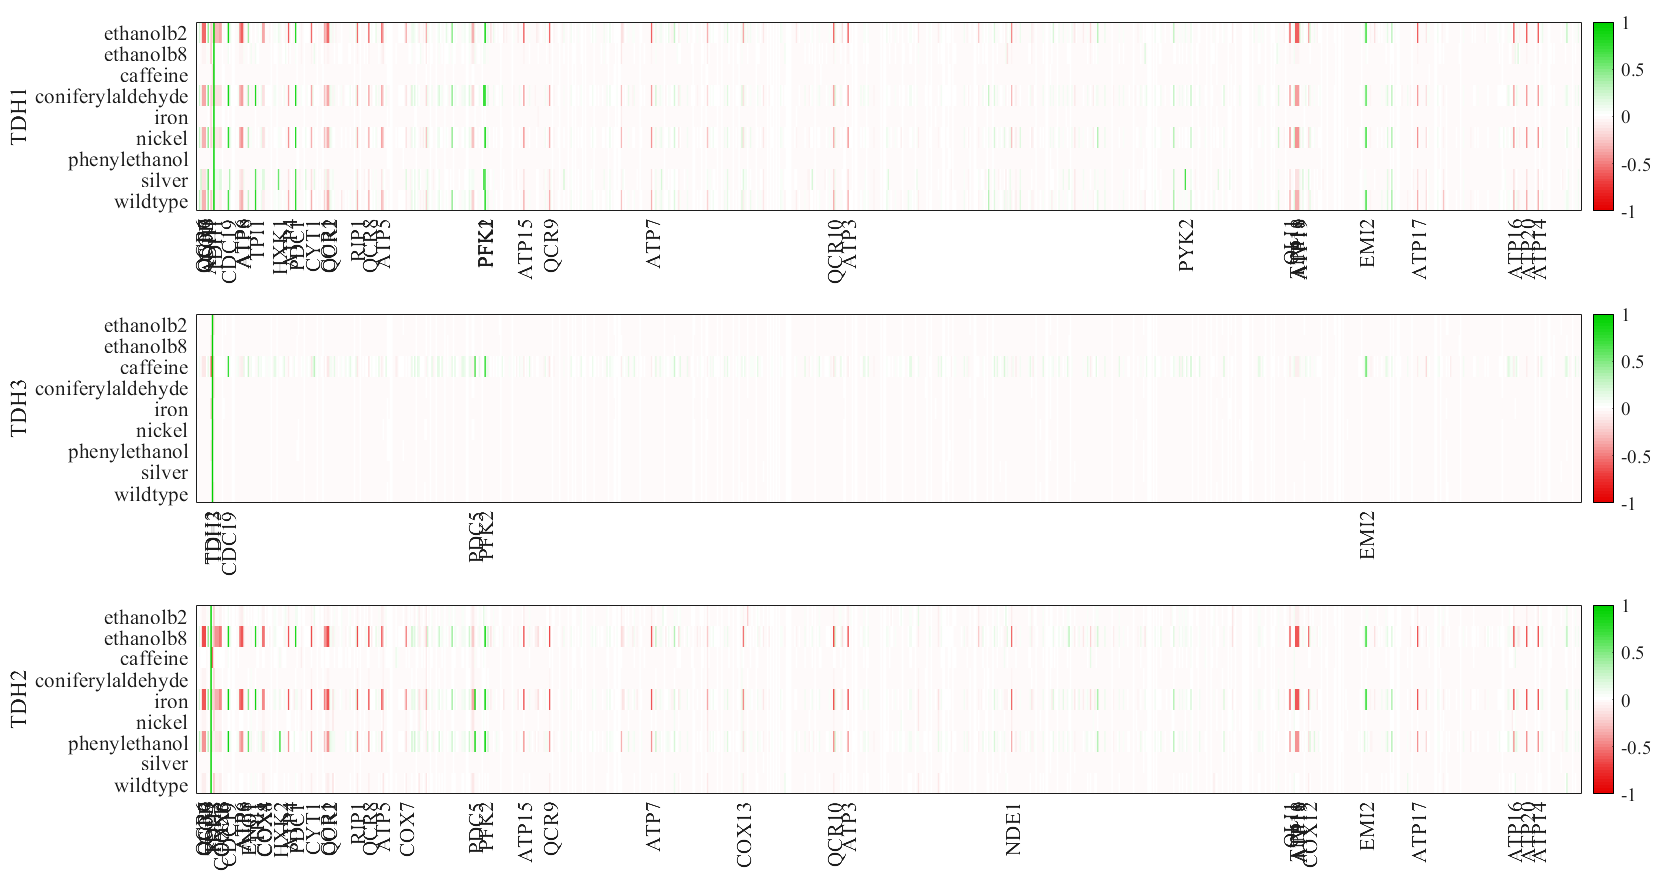
\includegraphics[width=1\columnwidth]{figures/sampling_correlation_tdh.png}
  \caption[Correlations of TDH1 (top), TDH3 (middle) and TDH2 (bottom) enzymes to other enzymes calculated from the random sampling of solution spaces. Only the name of enzymes with the correlation value c$>$0.5 are shown in the y-axes]{Correlations of TDH1 (top), TDH3 (middle) and TDH2 (bottom) enzymes to other enzymes calculated from the random sampling of solution spaces. Only the name of enzymes with the correlation value c$>$0.5 are shown in the y-axes.}
  \label{fig:sampling_correlation_tdh}
  \end{center}
\end{figure}

\begin{figure}[H]
  \begin{center}
  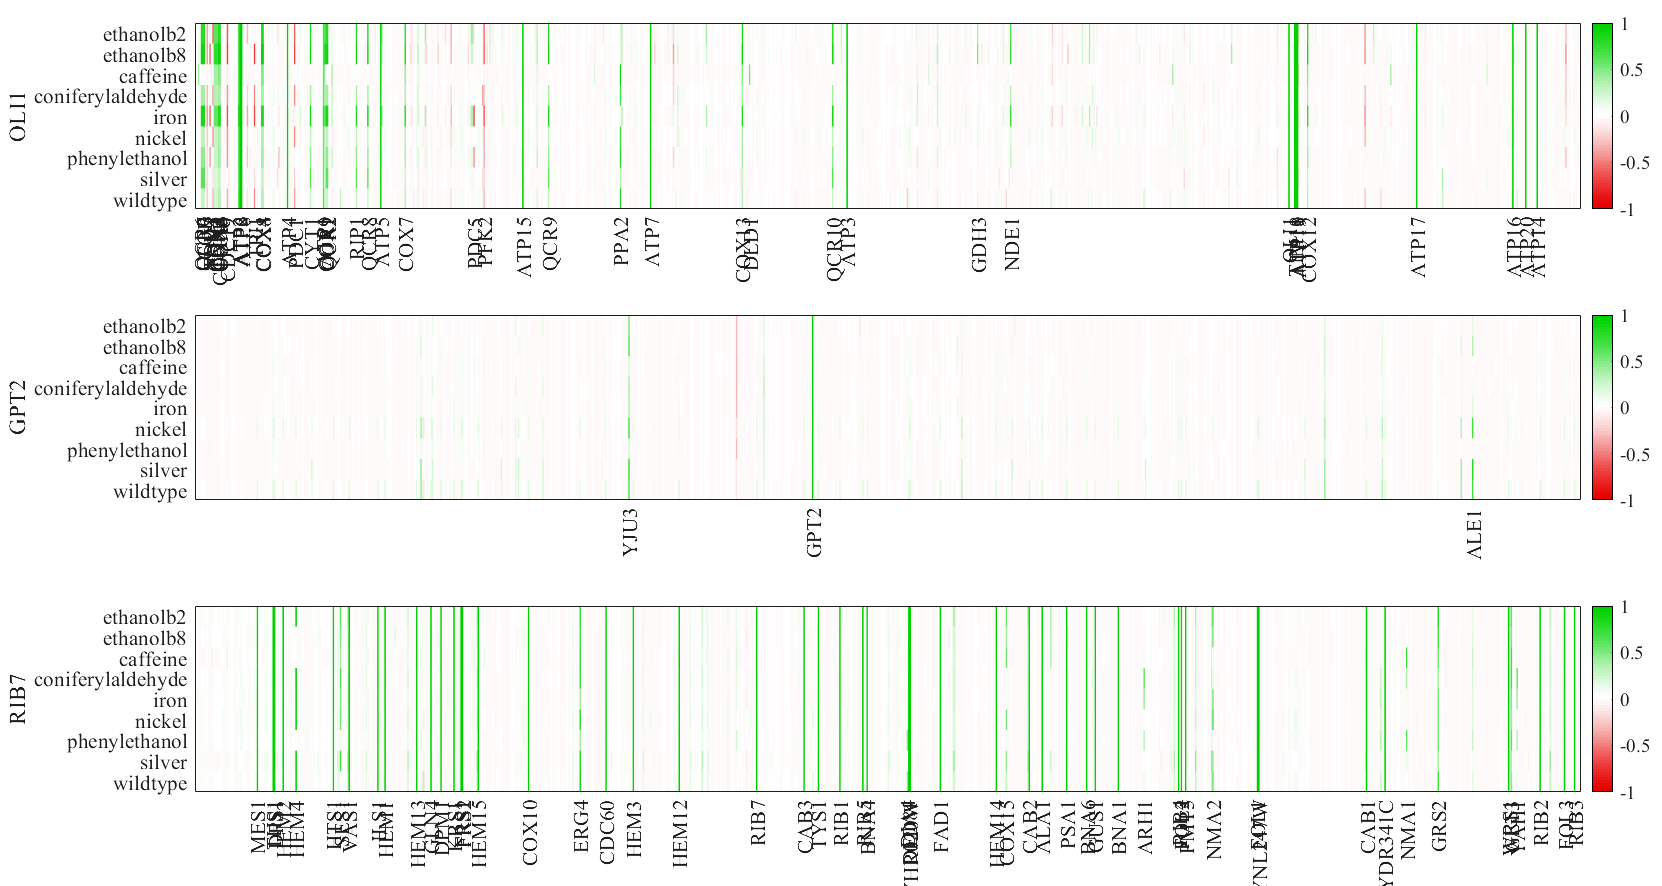
\includegraphics[width=1\columnwidth]{figures/sampling_correlation_oli_gpt_rib.png}
  \caption[Correlations of OLI1 (top), GPT2 (middle) and RIB7 (bottom) enzymes to other enzymes calculated from the random sampling of solution spaces. Only the name of enzymes with the correlation value c$>$0.5 are shown in the y-axes]{Correlations of OLI1 (top), GPT2 (middle) and RIB7 (bottom) enzymes to other enzymes calculated from the random sampling of solution spaces. Only the name of enzymes with the correlation value c$>$0.5 are shown in the y-axes.}
  \label{fig:sampling_correlation_oli_gpt_rib}
  \end{center}
\end{figure}

When we further investigate the enzymatic correlations of OLI1 (F0 ATP synthase subunit c), GPT2 (glycerol-3-phosphate/dihydroxyacetone phosphate sn-1 acyltransferase), and RIB7 (Diamino-hydroxy-phoshoribosyl-amino-pyrimidine deaminase) to other enzymes. We see that RIB7 shows similar results across models with the exception of correlations with HEM4 enzyme (uroporphyrinogen III synthase) absent in ethanolb8, caffeine and phenylethanol resistant models. Similar to HEM4 enzyme, COX15 (heme a synthase), ARH1 (mitochondrial oxidoreductase), NMA1 (nicotinic acid mononucleotide adenylyltransferase) and YAH1 (ferredoxin) enzymes must be investigated since they show different correlations across models although they are all involved in the heme biosynthesis pathways. In the case of OLI1, both positive and negative correlations are observed within all models, although the most distinct strain appears as caffeine resistant model by showying less correlations. GPT2 enzyme positively corralates with YJU3 (monoglyceride lipase) and ALE1 (lysophospholipid acyltransferase) enzymes in wildtype, silver and nickel resistant models with lower correlation values in caffeine resistant model.

\begin{figure}[H]
  \begin{center}
  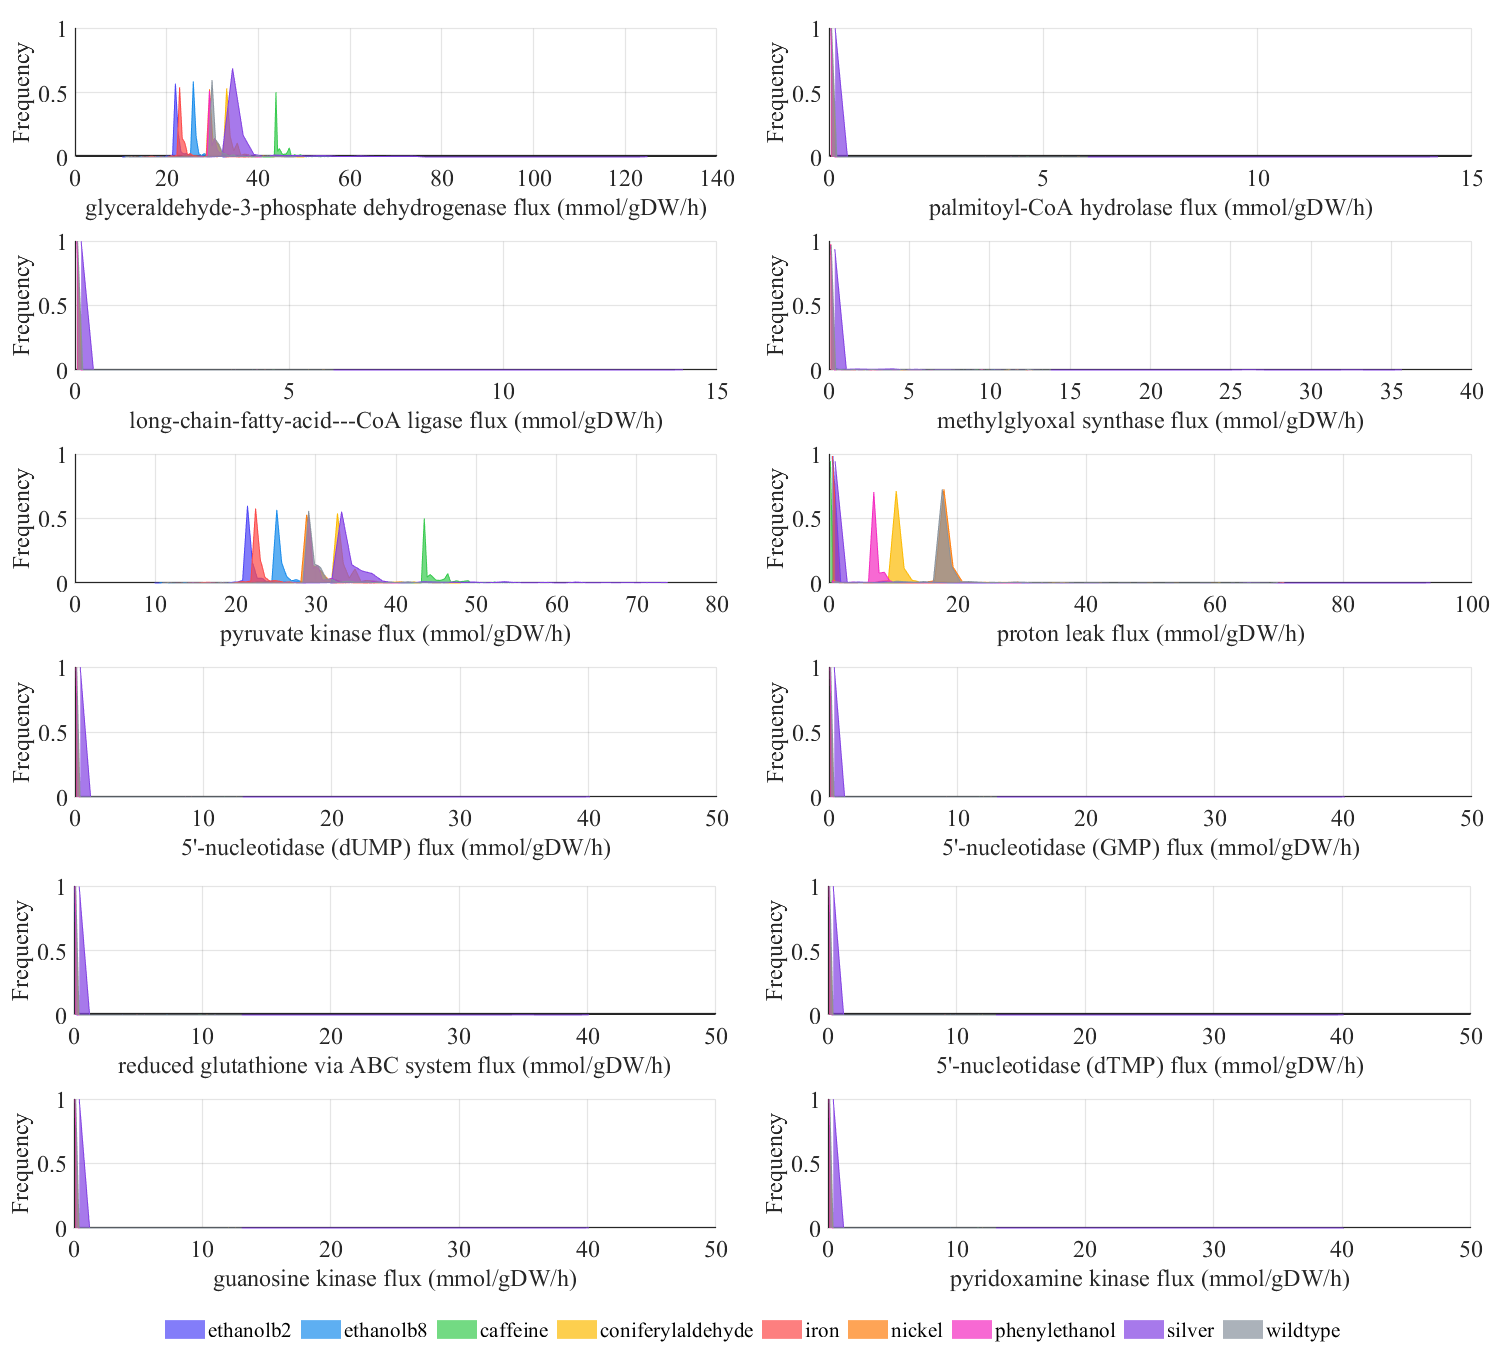
\includegraphics[width=1\columnwidth]{figures/sampling_moma_top12.png}
  \caption[Flux distributions of the reactions that diverge the most in the minimization of metabolic adjustment analysis, obtained from the random sampling of solution spaces for each model shown as histogram plots]{Flux distributions of the reactions that diverge the most in the minimization of metabolic adjustment analysis, obtained from the random sampling of solution spaces for each model shown as histogram plots.}
  \label{fig:sampling_moma_top12}
  \end{center}
\end{figure}

Glyceraldehyde-3-phosphate dehydrogenase reaction ranks once again #1 in a different analysis, MOMA. It can be seen that seperation is clear in all models with a wider flux range in the silver resistant model meaning that its flux value differ in multiple solutions. Followed by palmitoyl-CoA hydrolase, long chain fattyacid-CoA ligase and methylglyoxal synthase reactions are only in the Figure because they are only active in the silver resistant model. However since their flux ranges are too close to 0, they cannot be investigated as solid foundings. Pyruvate kinase reaction shows the same pattern as in previous analyses. Interestingly, proton leak reaction (leakage of hydrogen atoms from cytoplasm to mitochondria) carries flux up to 20 mmol/gDWh, indicating that in the phenylethanol, coniferylaldehyde and nickel resistant models, more than available proton is required in the mitochondria. Lastly, 5'-nucleotidase reactions, guanosine kinase and pyridoxamine kinase reactions are only active for silver resistant model, same as the previously mentioned reactions.

Finally, mean values for each enzyme from solution spaces are calculated. Z-scores are obtained from the difference between this means in each strain model to the wildtype model fluxes, divided by
the square root of the sum of standard deviations of this difference. Z-scores for enzymes are converted to p-values within gaussian distribution, and compared to the p-values obtained from the differential expression analysis. Discarding the non-significant enzymes in both cases, the following Figure \ref{fig:sampling_regulation_heatmaps} is constructed to compare regulations.

\begin{figure}[H]
  \begin{center}
  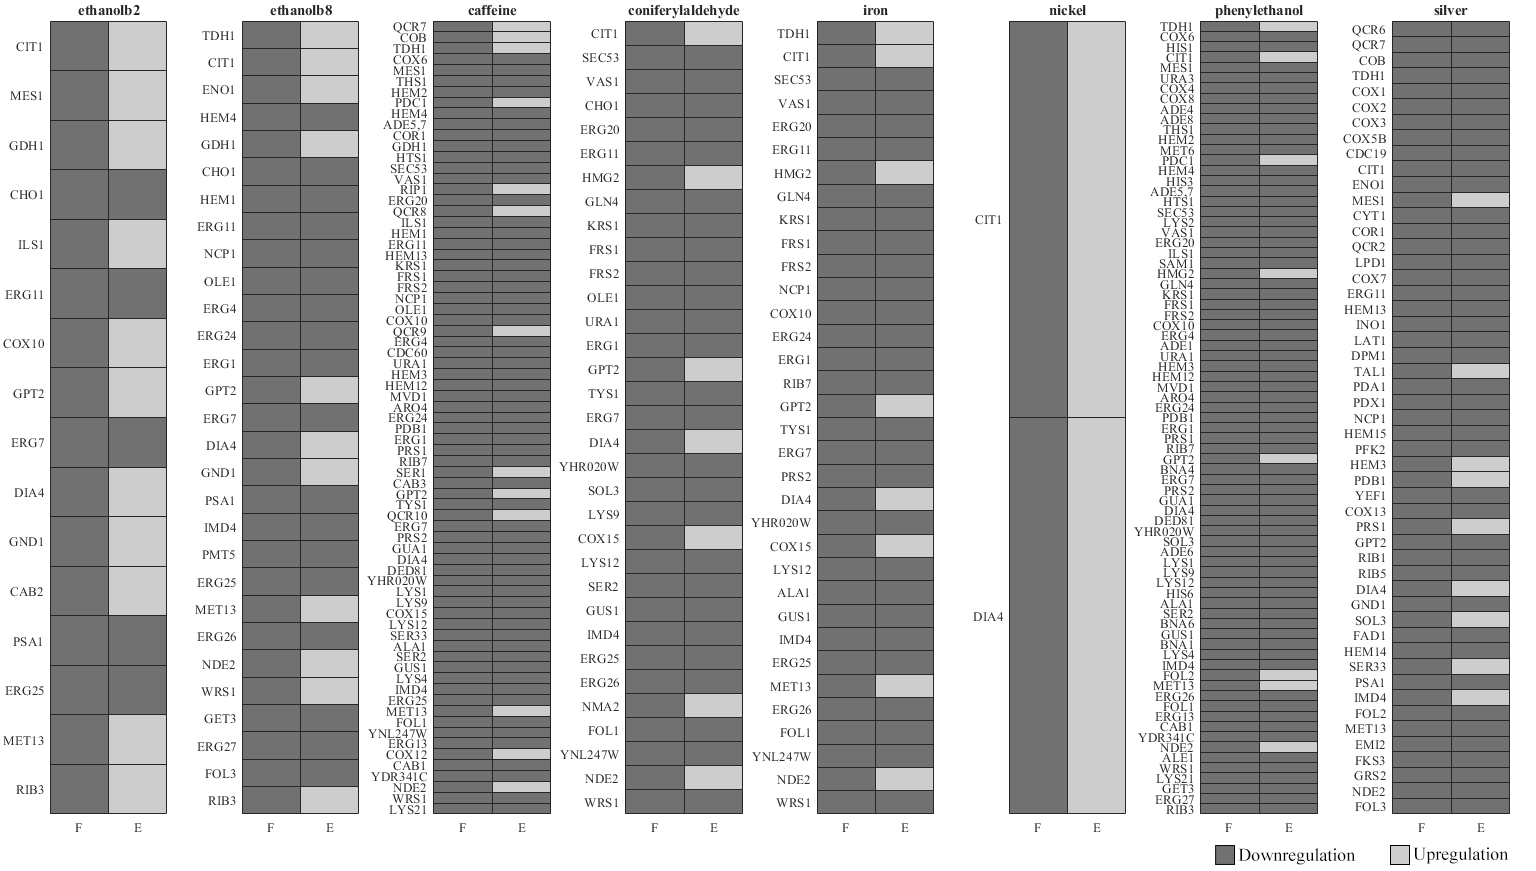
\includegraphics[width=1\columnwidth]{figures/sampling_regulation_heatmaps.png}
  \caption[Regulation of the enzymes obtained from the random sampling of solution spaces (F) and differential expression analysis (E) in all models. Enzymes that only have significant (p$<$0.05) changes are plotted in both flux and expression changes]{Regulation of the enzymes obtained from the random sampling of solution spaces (F) and differential expression analysis (E) in all models. Enzymes that only have significant (p$<$0.05) changes are plotted in both flux and expression changes. }
  \label{fig:sampling_regulation_heatmaps}
  \end{center}
\end{figure}

  \chapter{DISCUSSION}

In this work, genome-scale metabolic modelling methods are used to analyze transcriptomics of evolved \emph{S. cerevisiae} strains that have obtained by in vivo evolutionary engineering strategies for different environmental conditions where the following substances are gradually increased in the media: Ethanol, caffeine, coniferylaldehyde, iron, nickel, phenylethanol, and silver.

Turanlı-Yıldız et. al., obtained two evolved clones that could tolerate up to 12\% (v/v) ethanol, namely B2 and B8 strains, under increasing ethanol levels \cite{TuranlYldz2017}. Apart from the important findings on triggered diploidization during adaptation, their transcriptome analyses revealed that the most enriched genes were related to carbohydrates storage metabolism, however, only B2 strain alone exhibited a higher glycogen accumulation. They have also found that the abundances of mitochondrial proteins were decreased in B8 strain, suggesting a reduced respiratory activity. On top of that, findings on higher abundances of ribosomal proteins, amino acid metabolism, and glycolysis supported the idea of a higher fermentation levels.

In silico simulations show that, under the same environmental conditions provided, B2 strain is able to grow at slightly higher rates compared to B8 strain, 0.347 h\textsuperscript{-1} and 0.337 h\textsuperscript{-1} respectively, while B8 strain is able to produce ethanol at a higher rate 10.667 mmol/gDWh\textsuperscript{-1} compared to 9.934 mmol/gDWh\textsuperscript{-1} for B2 strain. The main difference observed in simulations between B2 and B8 strains is the regulation of citrate in the TCA cycle, specifically the transport reaction,
\begin{align}
\label{eq:citratetransport}
\ citrate_c + isocitrate_m \xleftrightarrow[\text{Rev: B8 (0.319 mmol/gDWh\textsuperscript{-1})}]{\text{Fwd: B2 (0.218 mmol/gDWh\textsuperscript{-1})}} citrate_m + isocitrate_c
\end{align}
\noindent where the indicators \emph{c} is for the cytoplasmic, and \emph{m} is for the mitochondrial metabolites. Transportation of citrate from mitochondria to cytoplasm in B8 strain agrees with the experimental findings on the idea of reduced respiratory activity, and this idea is supported with the ferrocytochrome-c:oxygen oxidoreductase (oxidative phosphorilation) fluxes where B2 strain has higher flux rate 18.867 mmol/gDWh\textsuperscript{-1}, compared to 17.439 mmol/gDWh\textsuperscript{-1} on B8 strain.

Although there is not a clear indicator on the glycogen synthase on simulations, the reason behind a slightly higher growth rate for B2 strain could arise from the carbohydrate pseudoreaction (Equation \ref{eq:carbohydratepseudo}) required for biomass. However, it must be noted that only 0.003 mmol/gDWh\textsuperscript{-1} difference is observet between B2 and B8 clones for the glycogen (starch) synthase reaction where UDP-D-glucose is converted into glycogen.
\begin{align}
\begin{split}
\label{eq:carbohydratepseudo}
\  0.74851 \text{ (1-3)-beta-D-glucan} + 0.25009 \text{ (1-6)-beta-D-glucan } + \\
\ 0.36141 \text{ glycogen} + 0.71094 \text{ mannan} + 0.13828 \text{ trehalose} \xrightarrow{}  \text{carbohydrate}
\end{split}
\end{align}

Sürmeli et. al., obtained yeast populations that can survive at high caffeine levels \cite{Srmeli2019}. Contrary to expectations from literature, their evolved strain, Caf905-2, did not show any inhibitory efects on the growth during stress selection. Transcriptome analysis on the obtained evolved strain, showed that Cytochrome c isoform 2 (CYC7) was the most upregulated gene. It is known that CYC7 is an electron carrier of the mitochondrial intermembrane space, and it is expressed under hypoxic conditions. In our simulations, we were able to catch the over-expression of CYC7 on flux variability analysis (Table \ref{table:fva_results}). Caffeine resistant model reaches to highest growth rate among evolved strains, and it was able to maintain energy without oxidative phosphorylation. As it can be seen from the phenotype phase planes in Figure \ref{fig:robustness_glu_oxy}, caffeine resistant model is highly sensitive oxygen availability and cannot grow if the oxygen uptake rate is higher than 25 mmol/gDWh\textsuperscript{-1}. Flux balance analysis shows that caffeine resistant model reaches its maximum available growth rate of 0.468 h\textsuperscript{-1} when the oxygen uptake rate is 0.235 mmol/gDWh\textsuperscript{-1}. In other words, the model choses not to take oxygen from outside if the carbon supply is unlimited in the media, it simulates hypoxic conditios for best outcome. However, if the glucose uptake is forced to 10 mmol/gDWh\textsuperscript{-1}, model takes more oxygen at the rate 4.757 mmol/gDWh\textsuperscript{-1}.

In their work, it has also been reported the induction of genes involved in glycogen and trehalose metabolism under cafeine stress. However, since the genome-scale modelling does not simulate stress conditions (i.e., no caffeine molecule is provided into the defined medium), this finding is not observed in the simulations, suggesting that this change could be regulated on the metabolic level, not on the transcriptomics level. Additionally, upregulation of SNQ2 was also not captured in the simulations, due to lack of its gene association in the Yeast8 model.

Transcriptomic changes in a coniferylaldehyde resistant yeast population, BH13, is reported by Hacısalihoğlu et. al., and differential regulations after adaptive evolution on the NAD(P)-dependent aldehyde dehydrogenases are revealed. They reported that all members of aldehyde dehydrogenases (ALD) except for ALD5 were upregulated, and ALD upregulation were previously observed in the literature \cite{adeboye2015catabolism}. Additionally, oxidoreductase enzymes such as BDH2, YPL113C, YJR096W; and putative aryl-alcohol dehydrogenases such as YPL088W and AAD15 were reported as upregulated in coniferylaldehyde resistant strain. Here, in flux variability analysis, ALD4 upregulation is observed in coniferylaldehyde resistant model, accompanied with the caffeine and phenylethanol resistant strains. From the experimental findings, cross-resistance were reported for the caffeine resistant strain for coniferylaldehyde stress, and a coniferylaldehyde resistant strain was also cross-resistant to cafeine stress. Considering this, our findings suggest that phenylethanol resistant strain may show a similar cross-resistance (experimental data on phenylethanol resistant strain is not published yet), and ALD gene family should be investigated in more detail. It is also observed that only these three (caffeine, coniferylaldehyde, and phenylethanol) models do not carry fluxes through fatty acid metabolism when the flux variability results are investigated pathway-wise.

In the coniferylaldehyde resistant strain, Hacısalihoğlu et. al. reported that the glucose uptake and metabolism were enhanced even without the coniferylaldehyde stress in the media \cite{Hacsaliholu2019}. This observation is explained by the upregulation of the genes encoding hexose transporters, and the enzymes involved in glycolysis, namely HXK1, GLK1, TDH1, GPM2, ERR1, and PYK2. Increased glucose uptake compared to wild-type model, and high flux range on flux variability analysis for HXK1, GLK1, and PYK2 in coniferylaldehyde resistant model confirms in silico simulations to the experimental findings. Similar to the results of ADL family, GLK1 enzyme has a higher flux range in caffeine and phenylethanol resistant models next to coniferylaldehyde resistant model. Interestingly, for the flux range of PYK2, iron resistant model accompanies coniferylaldehyde and caffeine resistant models instead of phenylethanol resistant model.


Iron resistant \emph{S. cerevisiae} mutant, M8FE, is obtained by Balaban et. al with cross resistance feature to other metals \cite{balaban2020evolutionary}, and their findings suggested that the resistance to the metals might be related to the downregulation of PHO84 gene, encoding a high-affinity inorganic phosphate transporter and also a low-affinity manganese transporter. Unfortunately, phosphate uptake rates show no significant difference on in silico simulations. In the experiments, it is assumed that high amounts of iron would lead to oxidative stress that damage the cells, however, ROS amounts of the evolved M8FE strain were lower compared to reference strain. This phenomena explained with the microarray results, where the upregulation on the oxidative stress response genes were observed. This upregulation is assumed to achieved in order to reduce oxidative levels in the cell. In the simulations, iron resistant model was able to grow at the same rate with the wildtype model when the maximum glucose uptake is allowed (Table \ref{table:growth_glucose_table}). However, when we consider ATP production, despite having high glucose uptake and growth rates as wildtype model, iron resistant model has much lower fluxes through ATP producing reactions compared to other models (Figure \ref{fig:fba_gro_glu_atp}). Although there is no in silico confirmation, Balaban et. al. suggests that the iron resistant strain prefers to save its energy as trehalose in the cell.

Their study also reported upregulations on the glycogen phosphorylase gene, GPH1; and phosphoglucomutase, PGM2. Here, flux variability analyses showed a high range for all evolved models for the enzyme PGM2, catalyst of the conversion from glucose-1-phosphate to glucose-6-phosphate, except in the silver resistant model. That being said, the upregulation in the PGM2 might possibly be related to DNA replication stress, and not a specific upregulation for the metal stress.



\subsection{Glyceraldehyde-3-phosphate dehydrogenase}
The most divergent enzyme through all evolved model simulations, glyceraldehyde-3-phosphate dehydrogenase (GAPDH) is an enzyme involved in glycolysis and gluconeogenesis pathways and it is encoded by three genes TDH1, TDH2 and TDH3 (triose-phosphate dehydrogenase; TDH) \cite{boucherie1995differential}. It catalyses the conversion of glyceraldehyde-3-phosphate to 1,3-bisphospho-D-glycerate during glycolysis and the reverse reaction during gluconeogenesis (Eq. \ref{eq:GAPDH}).
\begin{align}
\label{eq:GAPDH}
\begin{split}
\ \text{glyceraldehyde-3-phosphate} + NAD + P \leftrightarrow \\
\ \text{1,3-bisphospho-D-glycerate} + H^+ + NADH
\end{split}
\end{align}
In this study, it is found that carried flux through GAPDH is increased by 39\% in caffeine, 13\% in silver, and 11\% in coniferylaldehyde resistant model. On the contrary, the carried flux is decreased by 31\% in ethanolb2, 15\% in ethanolb8, and 26\% in iron resistant model. It is also observed that each evolved model uses different isozyme for the catalytic activity. GAPDH differences are summarized in Figure \ref{fig:discuss_GAPDH}.

For a long time, GAPDH was considered as an housekeeping gene for its constitutively expression in the cell, and commonly used in comparisons of expression data. In 2005, Barber et al. have reported different regulation mechanisms for GAPDH under specific conditions\cite{barber2005gapdh}, and it is later found that the gene is upregulated under hypoxic stress \cite{yang2008effects}. Additional functions in other cellular processes has also been described such as being a chaperone protein in cellular iron homeostasis \cite{sweeny2018glyceraldehyde}. Interestingly, catalytically active TDH enzymes are found in both the cytoplasm and the cell wall.

\begin{figure}[H]
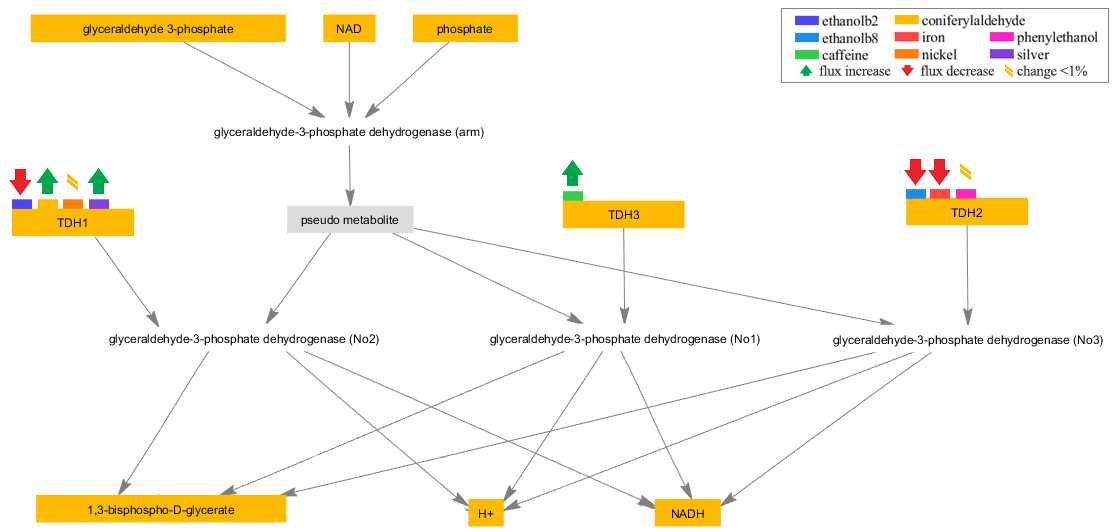
\includegraphics[width=1\columnwidth]{figures/discuss_GAPDH.png}
\caption[Map of glyceraldehyde-3-phosphate dehydrogenase catalized reaction as it used in simulations]{Map of glyceraldehyde-3-phosphate dehydrogenase catalized reaction as it used in simulations. Corresponding genes used for evolved models are shown in colors, and flux changes from wildtype model simulations are indicated as increased or decreased with arrows.}
\label{fig:discuss_GAPDH}
\end{figure}

GAPDH activity is controlled with oxygen availability, and evidence suggests that it may be the sensor of the cell in terms of oxidative stress \cite{chuang2005glyceraldehyde}. In the simulations presented here, oxidative phosphorylation through ATP synthase was totally inactive (zero flux) for the caffeine resistant model under unconstrained conditions, i.e., unlimited availability for uptake metabolites such as oxygen and glucose. Despite the inactivity, caffeine resistant model was the highest ATP producer among evolved models, and the ATP production was through pyruvate kinase and phosphoglycerate kinase activies (Table \ref{table:fba_atp_production}). Similar to caffeine resistant model, silver resistant model, too, showed increased activity on GAPDH and carried zero flux through ATP synthase in oxidative phosphorylation. In agreement with the results, ethanholb2, ethanolb8, and iron resistant models showed decreased activity for GAPDH and they were the only models that show ATP synthase activity.

  \chapter{EXPANDABLE TOPICS}

\section{Following will be added into introduction}, Toolboxes (such as COBRA, RAVEN or Other Softwares and Algorithms), FBA Methods (pFBA, dFBA, TFBA etc), Omics Data (subtopics for each omics, Model Integration Methods, Transcriptomics Analysis), metabolic control analysis...



	\bibliographystyle{styles/fbe_tez_v11}
	\bibliography{references}

\end{document}
